\documentclass{book}
\usepackage[a4paper,top=2.5cm,bottom=2.5cm,left=2.5cm,right=2.5cm]{geometry}
\usepackage{makeidx}
\usepackage{natbib}
\usepackage{graphicx}
\usepackage{multicol}
\usepackage{float}
\usepackage{listings}
\usepackage{color}
\usepackage{ifthen}
\usepackage[table]{xcolor}
\usepackage{textcomp}
\usepackage{alltt}
\usepackage{ifpdf}
\ifpdf
\usepackage[pdftex,
            pagebackref=true,
            colorlinks=true,
            linkcolor=blue,
            unicode
           ]{hyperref}
\else
\usepackage[ps2pdf,
            pagebackref=true,
            colorlinks=true,
            linkcolor=blue,
            unicode
           ]{hyperref}
\usepackage{pspicture}
\fi
\usepackage[utf8]{inputenc}
\usepackage{mathptmx}
\usepackage[scaled=.90]{helvet}
\usepackage{courier}
\usepackage{sectsty}
\usepackage{amssymb}
\usepackage[titles]{tocloft}
\usepackage{doxygen}
\lstset{language=C++,inputencoding=utf8,basicstyle=\footnotesize,breaklines=true,breakatwhitespace=true,tabsize=4,numbers=left }
\makeindex
\setcounter{tocdepth}{3}
\renewcommand{\footrulewidth}{0.4pt}
\renewcommand{\familydefault}{\sfdefault}
\hfuzz=15pt
\setlength{\emergencystretch}{15pt}
\hbadness=750
\tolerance=750
\begin{document}
\hypersetup{pageanchor=false,citecolor=blue}
\begin{titlepage}
\vspace*{7cm}
\begin{center}
{\Large Waveform\-Chassis Project }\\
\vspace*{1cm}
{\large Generated by Doxygen 1.8.2}\\
\vspace*{0.5cm}
{\small Sun Nov 11 2012 14:51:48}\\
\end{center}
\end{titlepage}
\clearemptydoublepage
\pagenumbering{roman}
\tableofcontents
\clearemptydoublepage
\pagenumbering{arabic}
\hypersetup{pageanchor=true,citecolor=blue}
\chapter{Hierarchical Index}
\section{Class Hierarchy}
This inheritance list is sorted roughly, but not completely, alphabetically\-:\begin{DoxyCompactList}
\item Exception\begin{DoxyCompactList}
\item \contentsline{section}{Chassis.\-git.\-D\-A\-Qmx\-Functions.\-D\-A\-Q\-Error}{\pageref{class_chassis_8git_1_1_d_a_qmx_functions_1_1_d_a_q_error}}{}
\item \contentsline{section}{Chassis.\-git.\-file\-Parser.\-file\-Parser\-Error}{\pageref{class_chassis_8git_1_1file_parser_1_1file_parser_error}}{}
\item \contentsline{section}{Chassis.\-git.\-ni\-Sync\-Error.\-ni\-Sync\-Error}{\pageref{class_chassis_8git_1_1ni_sync_error_1_1ni_sync_error}}{}
\end{DoxyCompactList}
\item object\begin{DoxyCompactList}
\item \contentsline{section}{Chassis.\-git.\-Analog\-Input.\-Analog\-Input}{\pageref{class_chassis_8git_1_1_analog_input_1_1_analog_input}}{}
\item \contentsline{section}{Chassis.\-git.\-Analog\-Output.\-Analog\-Output}{\pageref{class_chassis_8git_1_1_analog_output_1_1_analog_output}}{}
\item \contentsline{section}{Chassis.\-git.\-chassis\-Paths.\-chassis\-Paths}{\pageref{class_chassis_8git_1_1chassis_paths_1_1chassis_paths}}{}
\item \contentsline{section}{Chassis.\-git.\-D\-A\-Qmx\-Utility.\-Mode}{\pageref{class_chassis_8git_1_1_d_a_qmx_utility_1_1_mode}}{}
\item \contentsline{section}{Chassis.\-git.\-D\-A\-Qmx\-Utility.\-Trigger\-Type}{\pageref{class_chassis_8git_1_1_d_a_qmx_utility_1_1_trigger_type}}{}
\item \contentsline{section}{Chassis.\-git.\-dig\-Freq\-Generator.\-dig\-Freq\-Generator}{\pageref{class_chassis_8git_1_1dig_freq_generator_1_1dig_freq_generator}}{}
\item \contentsline{section}{Chassis.\-git.\-digital\-Buffer\-Manipulation.\-digital\-Buffer\-Manipulation}{\pageref{class_chassis_8git_1_1digital_buffer_manipulation_1_1digital_buffer_manipulation}}{}
\begin{DoxyCompactList}
\item \contentsline{section}{Chassis.\-git.\-digital\-Buffer\-Manipulation.\-digital\-Buffer\-Manipulation\-U16}{\pageref{class_chassis_8git_1_1digital_buffer_manipulation_1_1digital_buffer_manipulation_u16}}{}
\item \contentsline{section}{Chassis.\-git.\-digital\-Buffer\-Manipulation.\-digital\-Buffer\-Manipulation\-U8}{\pageref{class_chassis_8git_1_1digital_buffer_manipulation_1_1digital_buffer_manipulation_u8}}{}
\end{DoxyCompactList}
\item \contentsline{section}{Chassis.\-git.\-Digital\-Output.\-Digital\-Output}{\pageref{class_chassis_8git_1_1_digital_output_1_1_digital_output}}{}
\item \contentsline{section}{Chassis.\-git.\-dig\-Pulse\-Sequencer.\-dig\-Pulse\-Sequencer}{\pageref{class_chassis_8git_1_1dig_pulse_sequencer_1_1dig_pulse_sequencer}}{}
\item \contentsline{section}{Chassis.\-git.\-dig\-Pulse\-Sequencer.\-I\-Pulse\-Sequencer}{\pageref{class_chassis_8git_1_1dig_pulse_sequencer_1_1_i_pulse_sequencer}}{}
\item \contentsline{section}{Chassis.\-git.\-file\-Parser.\-file\-Parser}{\pageref{class_chassis_8git_1_1file_parser_1_1file_parser}}{}
\item \contentsline{section}{Chassis.\-git.\-p\-Counter.\-I\-Bin\-P\-Counter}{\pageref{class_chassis_8git_1_1p_counter_1_1_i_bin_p_counter}}{}
\item \contentsline{section}{Chassis.\-git.\-p\-Counter.\-p\-Counter}{\pageref{class_chassis_8git_1_1p_counter_1_1p_counter}}{}
\begin{DoxyCompactList}
\item \contentsline{section}{Chassis.\-git.\-p\-Counter.\-P\-Cntr\-Plot\-Dlg}{\pageref{class_chassis_8git_1_1p_counter_1_1_p_cntr_plot_dlg}}{}
\end{DoxyCompactList}
\item \contentsline{section}{Chassis.\-git.\-Timing.\-Timing}{\pageref{class_chassis_8git_1_1_timing_1_1_timing}}{}
\item \contentsline{section}{Chassis.\-git.\-Waveform\-Chassis.\-W\-C\-Low\-Level}{\pageref{class_chassis_8git_1_1_waveform_chassis_1_1_w_c_low_level}}{}
\begin{DoxyCompactList}
\item \contentsline{section}{Chassis.\-git.\-Waveform\-Chassis.\-Waveform\-Chassis}{\pageref{class_chassis_8git_1_1_waveform_chassis_1_1_waveform_chassis}}{}
\end{DoxyCompactList}
\item \contentsline{section}{Chassis.\-git.\-Waveform\-Generator.\-Waveform\-Generator}{\pageref{class_chassis_8git_1_1_waveform_generator_1_1_waveform_generator}}{}
\end{DoxyCompactList}
\item Auto\-Update\-Plot\begin{DoxyCompactList}
\item \contentsline{section}{Chassis.\-git.\-p\-Counter.\-P\-Cntr\-Plot\-Dlg}{\pageref{class_chassis_8git_1_1p_counter_1_1_p_cntr_plot_dlg}}{}
\end{DoxyCompactList}
\item file\-Parser\begin{DoxyCompactList}
\item \contentsline{section}{Chassis.\-git.\-e\-Map\-Parser.\-e\-Map\-Parser}{\pageref{class_chassis_8git_1_1e_map_parser_1_1e_map_parser}}{}
\item \contentsline{section}{Chassis.\-git.\-itf\-Parser.\-itf\-Parser}{\pageref{class_chassis_8git_1_1itf_parser_1_1itf_parser}}{}
\item \contentsline{section}{Chassis.\-git.\-Table\-File.\-Table\-File}{\pageref{class_chassis_8git_1_1_table_file_1_1_table_file}}{}
\end{DoxyCompactList}
\item Safe\-Config\-Parser\begin{DoxyCompactList}
\item \contentsline{section}{Chassis.\-git.\-chassis\-Config\-Parser.\-chassis\-Config\-Parser}{\pageref{class_chassis_8git_1_1chassis_config_parser_1_1chassis_config_parser}}{}
\end{DoxyCompactList}
\end{DoxyCompactList}

\chapter{Class Index}
\section{Class List}
Here are the classes, structs, unions and interfaces with brief descriptions\-:\begin{DoxyCompactList}
\item\contentsline{section}{\hyperlink{class_chassis_8git_1_1_analog_input_1_1_analog_input}{Chassis.\-git.\-Analog\-Input.\-Analog\-Input} \\*This class will acquire data from analog inputs useing py\-D\-A\-Qmx }{\pageref{class_chassis_8git_1_1_analog_input_1_1_analog_input}}{}
\item\contentsline{section}{\hyperlink{class_chassis_8git_1_1_analog_output_1_1_analog_output}{Chassis.\-git.\-Analog\-Output.\-Analog\-Output} \\*This class will generate analog outputs using py\-D\-A\-Qmx }{\pageref{class_chassis_8git_1_1_analog_output_1_1_analog_output}}{}
\item\contentsline{section}{\hyperlink{class_chassis_8git_1_1chassis_config_parser_1_1chassis_config_parser}{Chassis.\-git.\-chassis\-Config\-Parser.\-chassis\-Config\-Parser} \\*This class can read and write a Waveform\-Chassis configuration file }{\pageref{class_chassis_8git_1_1chassis_config_parser_1_1chassis_config_parser}}{}
\item\contentsline{section}{\hyperlink{class_chassis_8git_1_1chassis_paths_1_1chassis_paths}{Chassis.\-git.\-chassis\-Paths.\-chassis\-Paths} }{\pageref{class_chassis_8git_1_1chassis_paths_1_1chassis_paths}}{}
\item\contentsline{section}{\hyperlink{class_chassis_8git_1_1_d_a_qmx_functions_1_1_d_a_q_error}{Chassis.\-git.\-D\-A\-Qmx\-Functions.\-D\-A\-Q\-Error} }{\pageref{class_chassis_8git_1_1_d_a_qmx_functions_1_1_d_a_q_error}}{}
\item\contentsline{section}{\hyperlink{class_chassis_8git_1_1dig_freq_generator_1_1dig_freq_generator}{Chassis.\-git.\-dig\-Freq\-Generator.\-dig\-Freq\-Generator} }{\pageref{class_chassis_8git_1_1dig_freq_generator_1_1dig_freq_generator}}{}
\item\contentsline{section}{\hyperlink{class_chassis_8git_1_1digital_buffer_manipulation_1_1digital_buffer_manipulation}{Chassis.\-git.\-digital\-Buffer\-Manipulation.\-digital\-Buffer\-Manipulation} }{\pageref{class_chassis_8git_1_1digital_buffer_manipulation_1_1digital_buffer_manipulation}}{}
\item\contentsline{section}{\hyperlink{class_chassis_8git_1_1digital_buffer_manipulation_1_1digital_buffer_manipulation_u16}{Chassis.\-git.\-digital\-Buffer\-Manipulation.\-digital\-Buffer\-Manipulation\-U16} }{\pageref{class_chassis_8git_1_1digital_buffer_manipulation_1_1digital_buffer_manipulation_u16}}{}
\item\contentsline{section}{\hyperlink{class_chassis_8git_1_1digital_buffer_manipulation_1_1digital_buffer_manipulation_u8}{Chassis.\-git.\-digital\-Buffer\-Manipulation.\-digital\-Buffer\-Manipulation\-U8} }{\pageref{class_chassis_8git_1_1digital_buffer_manipulation_1_1digital_buffer_manipulation_u8}}{}
\item\contentsline{section}{\hyperlink{class_chassis_8git_1_1_digital_output_1_1_digital_output}{Chassis.\-git.\-Digital\-Output.\-Digital\-Output} \\*This class will generate digital outputs using py\-D\-A\-Qmx }{\pageref{class_chassis_8git_1_1_digital_output_1_1_digital_output}}{}
\item\contentsline{section}{\hyperlink{class_chassis_8git_1_1dig_pulse_sequencer_1_1dig_pulse_sequencer}{Chassis.\-git.\-dig\-Pulse\-Sequencer.\-dig\-Pulse\-Sequencer} }{\pageref{class_chassis_8git_1_1dig_pulse_sequencer_1_1dig_pulse_sequencer}}{}
\item\contentsline{section}{\hyperlink{class_chassis_8git_1_1e_map_parser_1_1e_map_parser}{Chassis.\-git.\-e\-Map\-Parser.\-e\-Map\-Parser} \\*This class will parse the electrode mape file }{\pageref{class_chassis_8git_1_1e_map_parser_1_1e_map_parser}}{}
\item\contentsline{section}{\hyperlink{class_chassis_8git_1_1file_parser_1_1file_parser}{Chassis.\-git.\-file\-Parser.\-file\-Parser} \\*This class is the parent class of all file parsers }{\pageref{class_chassis_8git_1_1file_parser_1_1file_parser}}{}
\item\contentsline{section}{\hyperlink{class_chassis_8git_1_1file_parser_1_1file_parser_error}{Chassis.\-git.\-file\-Parser.\-file\-Parser\-Error} \\*This is a class that creates a specific exception for the \hyperlink{class_chassis_8git_1_1file_parser_1_1file_parser}{file\-Parser} class }{\pageref{class_chassis_8git_1_1file_parser_1_1file_parser_error}}{}
\item\contentsline{section}{\hyperlink{class_chassis_8git_1_1p_counter_1_1_i_bin_p_counter}{Chassis.\-git.\-p\-Counter.\-I\-Bin\-P\-Counter} }{\pageref{class_chassis_8git_1_1p_counter_1_1_i_bin_p_counter}}{}
\item\contentsline{section}{\hyperlink{class_chassis_8git_1_1dig_pulse_sequencer_1_1_i_pulse_sequencer}{Chassis.\-git.\-dig\-Pulse\-Sequencer.\-I\-Pulse\-Sequencer} }{\pageref{class_chassis_8git_1_1dig_pulse_sequencer_1_1_i_pulse_sequencer}}{}
\item\contentsline{section}{\hyperlink{class_chassis_8git_1_1itf_parser_1_1itf_parser}{Chassis.\-git.\-itf\-Parser.\-itf\-Parser} \\*This class will parse through an itf file }{\pageref{class_chassis_8git_1_1itf_parser_1_1itf_parser}}{}
\item\contentsline{section}{\hyperlink{class_chassis_8git_1_1_d_a_qmx_utility_1_1_mode}{Chassis.\-git.\-D\-A\-Qmx\-Utility.\-Mode} \\*This class defines the mode variable which is used as an enumerated typedef }{\pageref{class_chassis_8git_1_1_d_a_qmx_utility_1_1_mode}}{}
\item\contentsline{section}{\hyperlink{class_chassis_8git_1_1ni_sync_error_1_1ni_sync_error}{Chassis.\-git.\-ni\-Sync\-Error.\-ni\-Sync\-Error} \\*This is a class to handle errors generated by the ni\-Sync python module }{\pageref{class_chassis_8git_1_1ni_sync_error_1_1ni_sync_error}}{}
\item\contentsline{section}{\hyperlink{class_chassis_8git_1_1p_counter_1_1_p_cntr_plot_dlg}{Chassis.\-git.\-p\-Counter.\-P\-Cntr\-Plot\-Dlg} }{\pageref{class_chassis_8git_1_1p_counter_1_1_p_cntr_plot_dlg}}{}
\item\contentsline{section}{\hyperlink{class_chassis_8git_1_1p_counter_1_1p_counter}{Chassis.\-git.\-p\-Counter.\-p\-Counter} \\*This class will count edges of a ditial signal at a sample clock rate specified, and has capability of being triggered to start }{\pageref{class_chassis_8git_1_1p_counter_1_1p_counter}}{}
\item\contentsline{section}{\hyperlink{class_chassis_8git_1_1_table_file_1_1_table_file}{Chassis.\-git.\-Table\-File.\-Table\-File} }{\pageref{class_chassis_8git_1_1_table_file_1_1_table_file}}{}
\item\contentsline{section}{\hyperlink{class_chassis_8git_1_1_timing_1_1_timing}{Chassis.\-git.\-Timing.\-Timing} \\*This class will generate perform the timing and synchronization required to synchronize all cards on the P\-X\-I backplane }{\pageref{class_chassis_8git_1_1_timing_1_1_timing}}{}
\item\contentsline{section}{\hyperlink{class_chassis_8git_1_1_d_a_qmx_utility_1_1_trigger_type}{Chassis.\-git.\-D\-A\-Qmx\-Utility.\-Trigger\-Type} \\*This class defines the trigger type variable which is used as an enumerated typedef }{\pageref{class_chassis_8git_1_1_d_a_qmx_utility_1_1_trigger_type}}{}
\item\contentsline{section}{\hyperlink{class_chassis_8git_1_1_waveform_chassis_1_1_waveform_chassis}{Chassis.\-git.\-Waveform\-Chassis.\-Waveform\-Chassis} \\*This class contains a list of Waveform\-Generator objects and a Timing object }{\pageref{class_chassis_8git_1_1_waveform_chassis_1_1_waveform_chassis}}{}
\item\contentsline{section}{\hyperlink{class_chassis_8git_1_1_waveform_generator_1_1_waveform_generator}{Chassis.\-git.\-Waveform\-Generator.\-Waveform\-Generator} \\*This class contains an Analog\-Output and Digital\-Output object }{\pageref{class_chassis_8git_1_1_waveform_generator_1_1_waveform_generator}}{}
\item\contentsline{section}{\hyperlink{class_chassis_8git_1_1_waveform_chassis_1_1_w_c_low_level}{Chassis.\-git.\-Waveform\-Chassis.\-W\-C\-Low\-Level} \\*This class contains a list of Waveform\-Generator objects and a Timing object }{\pageref{class_chassis_8git_1_1_waveform_chassis_1_1_w_c_low_level}}{}
\end{DoxyCompactList}

\chapter{Class Documentation}
\hypertarget{class_analog_output_1_1_analog_output}{\section{Analog\-Output.\-Analog\-Output Class Reference}
\label{class_analog_output_1_1_analog_output}\index{Analog\-Output.\-Analog\-Output@{Analog\-Output.\-Analog\-Output}}
}


This class will generate analog outputs using py\-D\-A\-Qmx.  


Inheritance diagram for Analog\-Output.\-Analog\-Output\-:\begin{figure}[H]
\begin{center}
\leavevmode
\includegraphics[height=2.000000cm]{class_analog_output_1_1_analog_output}
\end{center}
\end{figure}
\subsection*{Public Member Functions}
\begin{DoxyCompactItemize}
\item 
def \hyperlink{class_analog_output_1_1_analog_output_ad28820600816961e92acc55b7e87d8a3}{\-\_\-\-\_\-init\-\_\-\-\_\-}
\begin{DoxyCompactList}\small\item\em This function is a constructor for the \hyperlink{class_analog_output_1_1_analog_output}{Analog\-Output} class. \end{DoxyCompactList}\item 
def \hyperlink{class_analog_output_1_1_analog_output_ac2ebaea4a20d5a754b7758a322dcd317}{init}
\begin{DoxyCompactList}\small\item\em Initializes the analog outputs based on the object's configuration. \end{DoxyCompactList}\item 
def \hyperlink{class_analog_output_1_1_analog_output_a35ddeee69fe87b9956ba34a6a074e0ba}{get\-Samples\-Per\-Channel}
\begin{DoxyCompactList}\small\item\em This function returns the samples per channel configured in the D\-A\-Qmx Task. \end{DoxyCompactList}\item 
def \hyperlink{class_analog_output_1_1_analog_output_a090644cc9f7eb89e773c8e290c39e7fc}{set\-Samples\-Per\-Channel}
\begin{DoxyCompactList}\small\item\em This function sets the samples per channel in the D\-A\-Qmx Task. \end{DoxyCompactList}\item 
def \hyperlink{class_analog_output_1_1_analog_output_a82c8ed528235961775dd386c7fab6587}{get\-Clk\-Source}
\begin{DoxyCompactList}\small\item\em This function returns the sample clock source configured in the D\-A\-Qmx Task. \end{DoxyCompactList}\item 
def \hyperlink{class_analog_output_1_1_analog_output_a888663bef5a41818e2dadca65c56f4fc}{set\-Clk\-Source}
\begin{DoxyCompactList}\small\item\em This function sets the sample clock source in the D\-A\-Qmx Task. \end{DoxyCompactList}\item 
def \hyperlink{class_analog_output_1_1_analog_output_adcb04886fe1b222cbbf4ec8ab3c01153}{get\-Start\-Trigger\-Source}
\begin{DoxyCompactList}\small\item\em This function return the start trigger source configured in the D\-A\-Qmx Task. \end{DoxyCompactList}\item 
def \hyperlink{class_analog_output_1_1_analog_output_a9dacc2895d366a28732d480fd632ad80}{set\-Start\-Trigger\-Source}
\begin{DoxyCompactList}\small\item\em This function sets the start trigger source in the D\-A\-Qmx Task. \end{DoxyCompactList}\item 
def \hyperlink{class_analog_output_1_1_analog_output_af833d97ef4cb7cc53ac7eba7e69eb1ad}{get\-Num\-Channels}
\begin{DoxyCompactList}\small\item\em This function returns the number of channels configured in the D\-A\-Qmx Task. \end{DoxyCompactList}\item 
def \hyperlink{class_analog_output_1_1_analog_output_a19e38c3a77a064c52db37c48099684ce}{get\-Sample\-Rate}
\begin{DoxyCompactList}\small\item\em This function returns the sample rate configured in the D\-A\-Qmx Task. \end{DoxyCompactList}\item 
def \hyperlink{class_analog_output_1_1_analog_output_a20285eba22830949eb40ce15270655dd}{set\-Sample\-Rate}
\begin{DoxyCompactList}\small\item\em This funciton sets the sample rate in the D\-A\-Qmx Task. \end{DoxyCompactList}\item 
def \hyperlink{class_analog_output_1_1_analog_output_ae3fae0e7f57f4576cb2b3746c0873f50}{create\-Test\-Buffer}
\begin{DoxyCompactList}\small\item\em This function returns a 1\-D numpy array of samples with random voltages. \end{DoxyCompactList}\item 
def \hyperlink{class_analog_output_1_1_analog_output_aacf14b2f94fad32a659d1bd04b88ffd6}{create\-Sine\-Test\-Buffer}
\begin{DoxyCompactList}\small\item\em This function returns a 1\-D numpy array of sine waves. \end{DoxyCompactList}\item 
def \hyperlink{class_analog_output_1_1_analog_output_abd580af62942a68e3a453f8cfe499acb}{write\-To\-Buffer}
\begin{DoxyCompactList}\small\item\em This function writes the specified values into the buffer. \end{DoxyCompactList}\item 
def \hyperlink{class_analog_output_1_1_analog_output_a81a248ecf2eb72256cb58979e752e712}{start}
\begin{DoxyCompactList}\small\item\em This function starts the analog output generation. \end{DoxyCompactList}\item 
def \hyperlink{class_analog_output_1_1_analog_output_aa88017f59be11baa9c4284e9a7b39bbe}{wait\-Until\-Done}
\begin{DoxyCompactList}\small\item\em This functions waits for the analog output generation to complete. \end{DoxyCompactList}\item 
def \hyperlink{class_analog_output_1_1_analog_output_ae8b99d08fc29d3ff472824430ebd4067}{stop}
\begin{DoxyCompactList}\small\item\em This function stops the analog output generation. \end{DoxyCompactList}\item 
def \hyperlink{class_analog_output_1_1_analog_output_a483e645ff5fc84cd5f9cf4b146d9af0e}{close}
\begin{DoxyCompactList}\small\item\em This function will close connection to the analog ouput device and channels. \end{DoxyCompactList}\item 
def \hyperlink{class_analog_output_1_1_analog_output_a09b8b0f6cb839a7f00d45129340e5bea}{\-\_\-\-\_\-del\-\_\-\-\_\-}
\begin{DoxyCompactList}\small\item\em This is the destructor for the \hyperlink{class_analog_output_1_1_analog_output}{Analog\-Output} Class. \end{DoxyCompactList}\end{DoxyCompactItemize}
\subsection*{Public Attributes}
\begin{DoxyCompactItemize}
\item 
\hyperlink{class_analog_output_1_1_analog_output_a9244a764a26db3ca994e95f2e64f650f}{task\-Ref}
\begin{DoxyCompactList}\small\item\em The D\-A\-Qmx task reference. \end{DoxyCompactList}\item 
\hyperlink{class_analog_output_1_1_analog_output_aff699a66c410a728e70631b2e5e621a2}{initialized}
\begin{DoxyCompactList}\small\item\em This is a boolean that is true when the D\-A\-Qmx task has been initialized. \end{DoxyCompactList}\item 
\hyperlink{class_analog_output_1_1_analog_output_a021dd1434ccfaaa5a876ebde88609cb1}{status}
\begin{DoxyCompactList}\small\item\em This is the status of the D\-A\-Qmx task. \end{DoxyCompactList}\item 
\hyperlink{class_analog_output_1_1_analog_output_a7f2d56d4169a65eb67d1f5d3f2c5c87a}{start\-Trigger\-Sync\-Card}
\begin{DoxyCompactList}\small\item\em This is the start trigger terminal of the N\-I-\/\-Sync card. \end{DoxyCompactList}\item 
\hyperlink{class_analog_output_1_1_analog_output_aac2f3b8aa6e295ee91e3671c57c68e47}{mode}
\begin{DoxyCompactList}\small\item\em This is the mode of operation for the analog outputs. \end{DoxyCompactList}\item 
\hyperlink{class_analog_output_1_1_analog_output_a760ab1469dad131efc3a61354dd59db3}{trigger\-Type}
\begin{DoxyCompactList}\small\item\em The trigger type for the analog outputs. \end{DoxyCompactList}\item 
\hyperlink{class_analog_output_1_1_analog_output_a6ef94f02074244f9f6c513fd25208b46}{loops}
\begin{DoxyCompactList}\small\item\em The number of times to iterate over a Finite number of samples. \end{DoxyCompactList}\item 
\hyperlink{class_analog_output_1_1_analog_output_a00b63231e0b6b1fcd479b140616eb573}{est\-Acq\-Time}
\begin{DoxyCompactList}\small\item\em The estimated time to generate the samples for a Finite generation. \end{DoxyCompactList}\end{DoxyCompactItemize}
\subsection*{Properties}
\begin{DoxyCompactItemize}
\item 
\hyperlink{class_analog_output_1_1_analog_output_a3b52a2dd204f53dd5e5573011c1399e8}{samples\-Per\-Channel}
\begin{DoxyCompactList}\small\item\em This is the number of samples per channel that will be generated in Finite mode. \end{DoxyCompactList}\item 
\hyperlink{class_analog_output_1_1_analog_output_ab35cc7e572968599d8f2fc4df8e3d7e2}{clk\-Source} property(\hyperlink{class_analog_output_1_1_analog_output_a82c8ed528235961775dd386c7fab6587}{get\-Clk\-Source}, \hyperlink{class_analog_output_1_1_analog_output_a888663bef5a41818e2dadca65c56f4fc}{set\-Clk\-Source}, \-\_\-del\-Clk\-Source)
\begin{DoxyCompactList}\small\item\em This is the sample clock source terminal. \end{DoxyCompactList}\item 
\hyperlink{class_analog_output_1_1_analog_output_a6fb285ae88ea470ec5a99f9163e36c88}{start\-Trigger\-Source} property(\hyperlink{class_analog_output_1_1_analog_output_adcb04886fe1b222cbbf4ec8ab3c01153}{get\-Start\-Trigger\-Source}, \hyperlink{class_analog_output_1_1_analog_output_a9dacc2895d366a28732d480fd632ad80}{set\-Start\-Trigger\-Source}, \-\_\-del\-Start\-Trigger\-Source)
\begin{DoxyCompactList}\small\item\em This is the start trigger source terminal. \end{DoxyCompactList}\item 
\hyperlink{class_analog_output_1_1_analog_output_a0ca884b5b69a1e37758b6ea74f5e2b6f}{num\-Channels} property(\hyperlink{class_analog_output_1_1_analog_output_af833d97ef4cb7cc53ac7eba7e69eb1ad}{get\-Num\-Channels})
\begin{DoxyCompactList}\small\item\em This is the number of channels configured in the task. \end{DoxyCompactList}\item 
\hyperlink{class_analog_output_1_1_analog_output_a493b9db1346a6d9cceae925ad85a3fef}{sample\-Rate} property(\hyperlink{class_analog_output_1_1_analog_output_a19e38c3a77a064c52db37c48099684ce}{get\-Sample\-Rate}, \hyperlink{class_analog_output_1_1_analog_output_a20285eba22830949eb40ce15270655dd}{set\-Sample\-Rate}, \-\_\-del\-Sample\-Rate)
\begin{DoxyCompactList}\small\item\em This is the sample rate of the analog output. \end{DoxyCompactList}\end{DoxyCompactItemize}


\subsection{Detailed Description}
This class will generate analog outputs using py\-D\-A\-Qmx. 



\subsection{Constructor \& Destructor Documentation}
\hypertarget{class_analog_output_1_1_analog_output_ad28820600816961e92acc55b7e87d8a3}{\index{Analog\-Output\-::\-Analog\-Output@{Analog\-Output\-::\-Analog\-Output}!\-\_\-\-\_\-init\-\_\-\-\_\-@{\-\_\-\-\_\-init\-\_\-\-\_\-}}
\index{\-\_\-\-\_\-init\-\_\-\-\_\-@{\-\_\-\-\_\-init\-\_\-\-\_\-}!AnalogOutput::AnalogOutput@{Analog\-Output\-::\-Analog\-Output}}
\subsubsection[{\-\_\-\-\_\-init\-\_\-\-\_\-}]{\setlength{\rightskip}{0pt plus 5cm}def Analog\-Output.\-Analog\-Output.\-\_\-\-\_\-init\-\_\-\-\_\- (
\begin{DoxyParamCaption}
\item[{}]{self}
\end{DoxyParamCaption}
)}}\label{class_analog_output_1_1_analog_output_ad28820600816961e92acc55b7e87d8a3}


This function is a constructor for the \hyperlink{class_analog_output_1_1_analog_output}{Analog\-Output} class. 

It creates the internal variables required to perform functions within the class. This function does not initialize any hardware. \hypertarget{class_analog_output_1_1_analog_output_a09b8b0f6cb839a7f00d45129340e5bea}{\index{Analog\-Output\-::\-Analog\-Output@{Analog\-Output\-::\-Analog\-Output}!\-\_\-\-\_\-del\-\_\-\-\_\-@{\-\_\-\-\_\-del\-\_\-\-\_\-}}
\index{\-\_\-\-\_\-del\-\_\-\-\_\-@{\-\_\-\-\_\-del\-\_\-\-\_\-}!AnalogOutput::AnalogOutput@{Analog\-Output\-::\-Analog\-Output}}
\subsubsection[{\-\_\-\-\_\-del\-\_\-\-\_\-}]{\setlength{\rightskip}{0pt plus 5cm}def Analog\-Output.\-Analog\-Output.\-\_\-\-\_\-del\-\_\-\-\_\- (
\begin{DoxyParamCaption}
\item[{}]{self}
\end{DoxyParamCaption}
)}}\label{class_analog_output_1_1_analog_output_a09b8b0f6cb839a7f00d45129340e5bea}


This is the destructor for the \hyperlink{class_analog_output_1_1_analog_output}{Analog\-Output} Class. 


\begin{DoxyParams}{Parameters}
{\em self} & The object pointer. \\
\hline
\end{DoxyParams}


\subsection{Member Function Documentation}
\hypertarget{class_analog_output_1_1_analog_output_a483e645ff5fc84cd5f9cf4b146d9af0e}{\index{Analog\-Output\-::\-Analog\-Output@{Analog\-Output\-::\-Analog\-Output}!close@{close}}
\index{close@{close}!AnalogOutput::AnalogOutput@{Analog\-Output\-::\-Analog\-Output}}
\subsubsection[{close}]{\setlength{\rightskip}{0pt plus 5cm}def Analog\-Output.\-Analog\-Output.\-close (
\begin{DoxyParamCaption}
\item[{}]{self}
\end{DoxyParamCaption}
)}}\label{class_analog_output_1_1_analog_output_a483e645ff5fc84cd5f9cf4b146d9af0e}


This function will close connection to the analog ouput device and channels. 


\begin{DoxyParams}{Parameters}
{\em self} & The object pointer. \\
\hline
\end{DoxyParams}
\hypertarget{class_analog_output_1_1_analog_output_aacf14b2f94fad32a659d1bd04b88ffd6}{\index{Analog\-Output\-::\-Analog\-Output@{Analog\-Output\-::\-Analog\-Output}!create\-Sine\-Test\-Buffer@{create\-Sine\-Test\-Buffer}}
\index{create\-Sine\-Test\-Buffer@{create\-Sine\-Test\-Buffer}!AnalogOutput::AnalogOutput@{Analog\-Output\-::\-Analog\-Output}}
\subsubsection[{create\-Sine\-Test\-Buffer}]{\setlength{\rightskip}{0pt plus 5cm}def Analog\-Output.\-Analog\-Output.\-create\-Sine\-Test\-Buffer (
\begin{DoxyParamCaption}
\item[{}]{self}
\end{DoxyParamCaption}
)}}\label{class_analog_output_1_1_analog_output_aacf14b2f94fad32a659d1bd04b88ffd6}


This function returns a 1\-D numpy array of sine waves. 

The returned value is intended to be used to write samples to the buffer with the \hyperlink{class_analog_output_1_1_analog_output_abd580af62942a68e3a453f8cfe499acb}{write\-To\-Buffer()} method. 
\begin{DoxyParams}{Parameters}
{\em self} & The object pointer. \\
\hline
\end{DoxyParams}
\hypertarget{class_analog_output_1_1_analog_output_ae3fae0e7f57f4576cb2b3746c0873f50}{\index{Analog\-Output\-::\-Analog\-Output@{Analog\-Output\-::\-Analog\-Output}!create\-Test\-Buffer@{create\-Test\-Buffer}}
\index{create\-Test\-Buffer@{create\-Test\-Buffer}!AnalogOutput::AnalogOutput@{Analog\-Output\-::\-Analog\-Output}}
\subsubsection[{create\-Test\-Buffer}]{\setlength{\rightskip}{0pt plus 5cm}def Analog\-Output.\-Analog\-Output.\-create\-Test\-Buffer (
\begin{DoxyParamCaption}
\item[{}]{self, }
\item[{}]{num\-Channels = {\ttfamily 0}}
\end{DoxyParamCaption}
)}}\label{class_analog_output_1_1_analog_output_ae3fae0e7f57f4576cb2b3746c0873f50}


This function returns a 1\-D numpy array of samples with random voltages. 

The returned value is intended to be used to write samples to the buffer with the \hyperlink{class_analog_output_1_1_analog_output_abd580af62942a68e3a453f8cfe499acb}{write\-To\-Buffer()} method. 
\begin{DoxyParams}{Parameters}
{\em self} & The object pointer. \\
\hline
{\em num\-Channels} & The number of channels to generate. If this parameter is not provided, Then the function will generate the number of channels configured in the analog output task. \\
\hline
\end{DoxyParams}
\hypertarget{class_analog_output_1_1_analog_output_a82c8ed528235961775dd386c7fab6587}{\index{Analog\-Output\-::\-Analog\-Output@{Analog\-Output\-::\-Analog\-Output}!get\-Clk\-Source@{get\-Clk\-Source}}
\index{get\-Clk\-Source@{get\-Clk\-Source}!AnalogOutput::AnalogOutput@{Analog\-Output\-::\-Analog\-Output}}
\subsubsection[{get\-Clk\-Source}]{\setlength{\rightskip}{0pt plus 5cm}def Analog\-Output.\-Analog\-Output.\-get\-Clk\-Source (
\begin{DoxyParamCaption}
\item[{}]{self}
\end{DoxyParamCaption}
)}}\label{class_analog_output_1_1_analog_output_a82c8ed528235961775dd386c7fab6587}


This function returns the sample clock source configured in the D\-A\-Qmx Task. 


\begin{DoxyParams}{Parameters}
{\em self} & The object pointer. \\
\hline
\end{DoxyParams}
\hypertarget{class_analog_output_1_1_analog_output_af833d97ef4cb7cc53ac7eba7e69eb1ad}{\index{Analog\-Output\-::\-Analog\-Output@{Analog\-Output\-::\-Analog\-Output}!get\-Num\-Channels@{get\-Num\-Channels}}
\index{get\-Num\-Channels@{get\-Num\-Channels}!AnalogOutput::AnalogOutput@{Analog\-Output\-::\-Analog\-Output}}
\subsubsection[{get\-Num\-Channels}]{\setlength{\rightskip}{0pt plus 5cm}def Analog\-Output.\-Analog\-Output.\-get\-Num\-Channels (
\begin{DoxyParamCaption}
\item[{}]{self}
\end{DoxyParamCaption}
)}}\label{class_analog_output_1_1_analog_output_af833d97ef4cb7cc53ac7eba7e69eb1ad}


This function returns the number of channels configured in the D\-A\-Qmx Task. 


\begin{DoxyParams}{Parameters}
{\em self} & The object pointer. \\
\hline
\end{DoxyParams}
\hypertarget{class_analog_output_1_1_analog_output_a19e38c3a77a064c52db37c48099684ce}{\index{Analog\-Output\-::\-Analog\-Output@{Analog\-Output\-::\-Analog\-Output}!get\-Sample\-Rate@{get\-Sample\-Rate}}
\index{get\-Sample\-Rate@{get\-Sample\-Rate}!AnalogOutput::AnalogOutput@{Analog\-Output\-::\-Analog\-Output}}
\subsubsection[{get\-Sample\-Rate}]{\setlength{\rightskip}{0pt plus 5cm}def Analog\-Output.\-Analog\-Output.\-get\-Sample\-Rate (
\begin{DoxyParamCaption}
\item[{}]{self}
\end{DoxyParamCaption}
)}}\label{class_analog_output_1_1_analog_output_a19e38c3a77a064c52db37c48099684ce}


This function returns the sample rate configured in the D\-A\-Qmx Task. 


\begin{DoxyParams}{Parameters}
{\em self} & The object pointer. \\
\hline
\end{DoxyParams}
\hypertarget{class_analog_output_1_1_analog_output_a35ddeee69fe87b9956ba34a6a074e0ba}{\index{Analog\-Output\-::\-Analog\-Output@{Analog\-Output\-::\-Analog\-Output}!get\-Samples\-Per\-Channel@{get\-Samples\-Per\-Channel}}
\index{get\-Samples\-Per\-Channel@{get\-Samples\-Per\-Channel}!AnalogOutput::AnalogOutput@{Analog\-Output\-::\-Analog\-Output}}
\subsubsection[{get\-Samples\-Per\-Channel}]{\setlength{\rightskip}{0pt plus 5cm}def Analog\-Output.\-Analog\-Output.\-get\-Samples\-Per\-Channel (
\begin{DoxyParamCaption}
\item[{}]{self}
\end{DoxyParamCaption}
)}}\label{class_analog_output_1_1_analog_output_a35ddeee69fe87b9956ba34a6a074e0ba}


This function returns the samples per channel configured in the D\-A\-Qmx Task. 


\begin{DoxyParams}{Parameters}
{\em self} & The object pointer. \\
\hline
\end{DoxyParams}
\hypertarget{class_analog_output_1_1_analog_output_adcb04886fe1b222cbbf4ec8ab3c01153}{\index{Analog\-Output\-::\-Analog\-Output@{Analog\-Output\-::\-Analog\-Output}!get\-Start\-Trigger\-Source@{get\-Start\-Trigger\-Source}}
\index{get\-Start\-Trigger\-Source@{get\-Start\-Trigger\-Source}!AnalogOutput::AnalogOutput@{Analog\-Output\-::\-Analog\-Output}}
\subsubsection[{get\-Start\-Trigger\-Source}]{\setlength{\rightskip}{0pt plus 5cm}def Analog\-Output.\-Analog\-Output.\-get\-Start\-Trigger\-Source (
\begin{DoxyParamCaption}
\item[{}]{self}
\end{DoxyParamCaption}
)}}\label{class_analog_output_1_1_analog_output_adcb04886fe1b222cbbf4ec8ab3c01153}


This function return the start trigger source configured in the D\-A\-Qmx Task. 


\begin{DoxyParams}{Parameters}
{\em self} & The object pointer. \\
\hline
\end{DoxyParams}
\hypertarget{class_analog_output_1_1_analog_output_ac2ebaea4a20d5a754b7758a322dcd317}{\index{Analog\-Output\-::\-Analog\-Output@{Analog\-Output\-::\-Analog\-Output}!init@{init}}
\index{init@{init}!AnalogOutput::AnalogOutput@{Analog\-Output\-::\-Analog\-Output}}
\subsubsection[{init}]{\setlength{\rightskip}{0pt plus 5cm}def Analog\-Output.\-Analog\-Output.\-init (
\begin{DoxyParamCaption}
\item[{}]{self, }
\item[{}]{physical\-Channel}
\end{DoxyParamCaption}
)}}\label{class_analog_output_1_1_analog_output_ac2ebaea4a20d5a754b7758a322dcd317}


Initializes the analog outputs based on the object's configuration. 


\begin{DoxyParams}{Parameters}
{\em self} & The object pointer. \\
\hline
{\em physical\-Channel} & A string representing the device and analog output channels. Example Value\-: \char`\"{}\-P\-X\-I1\-Slot3/ao0\-:7\char`\"{} \\
\hline
\end{DoxyParams}
\hypertarget{class_analog_output_1_1_analog_output_a888663bef5a41818e2dadca65c56f4fc}{\index{Analog\-Output\-::\-Analog\-Output@{Analog\-Output\-::\-Analog\-Output}!set\-Clk\-Source@{set\-Clk\-Source}}
\index{set\-Clk\-Source@{set\-Clk\-Source}!AnalogOutput::AnalogOutput@{Analog\-Output\-::\-Analog\-Output}}
\subsubsection[{set\-Clk\-Source}]{\setlength{\rightskip}{0pt plus 5cm}def Analog\-Output.\-Analog\-Output.\-set\-Clk\-Source (
\begin{DoxyParamCaption}
\item[{}]{self, }
\item[{}]{value}
\end{DoxyParamCaption}
)}}\label{class_analog_output_1_1_analog_output_a888663bef5a41818e2dadca65c56f4fc}


This function sets the sample clock source in the D\-A\-Qmx Task. 


\begin{DoxyParams}{Parameters}
{\em self} & The object pointer. \\
\hline
{\em value} & The string value for the clock source terminal. \\
\hline
\end{DoxyParams}
\hypertarget{class_analog_output_1_1_analog_output_a20285eba22830949eb40ce15270655dd}{\index{Analog\-Output\-::\-Analog\-Output@{Analog\-Output\-::\-Analog\-Output}!set\-Sample\-Rate@{set\-Sample\-Rate}}
\index{set\-Sample\-Rate@{set\-Sample\-Rate}!AnalogOutput::AnalogOutput@{Analog\-Output\-::\-Analog\-Output}}
\subsubsection[{set\-Sample\-Rate}]{\setlength{\rightskip}{0pt plus 5cm}def Analog\-Output.\-Analog\-Output.\-set\-Sample\-Rate (
\begin{DoxyParamCaption}
\item[{}]{self, }
\item[{}]{value}
\end{DoxyParamCaption}
)}}\label{class_analog_output_1_1_analog_output_a20285eba22830949eb40ce15270655dd}


This funciton sets the sample rate in the D\-A\-Qmx Task. 


\begin{DoxyParams}{Parameters}
{\em self} & The object pointer. \\
\hline
{\em value} & The value of the sample rate. \\
\hline
\end{DoxyParams}
\hypertarget{class_analog_output_1_1_analog_output_a090644cc9f7eb89e773c8e290c39e7fc}{\index{Analog\-Output\-::\-Analog\-Output@{Analog\-Output\-::\-Analog\-Output}!set\-Samples\-Per\-Channel@{set\-Samples\-Per\-Channel}}
\index{set\-Samples\-Per\-Channel@{set\-Samples\-Per\-Channel}!AnalogOutput::AnalogOutput@{Analog\-Output\-::\-Analog\-Output}}
\subsubsection[{set\-Samples\-Per\-Channel}]{\setlength{\rightskip}{0pt plus 5cm}def Analog\-Output.\-Analog\-Output.\-set\-Samples\-Per\-Channel (
\begin{DoxyParamCaption}
\item[{}]{self, }
\item[{}]{value}
\end{DoxyParamCaption}
)}}\label{class_analog_output_1_1_analog_output_a090644cc9f7eb89e773c8e290c39e7fc}


This function sets the samples per channel in the D\-A\-Qmx Task. 


\begin{DoxyParams}{Parameters}
{\em self} & The object pointer. \\
\hline
{\em value} & The value to set the samples per channel. \\
\hline
\end{DoxyParams}
\hypertarget{class_analog_output_1_1_analog_output_a9dacc2895d366a28732d480fd632ad80}{\index{Analog\-Output\-::\-Analog\-Output@{Analog\-Output\-::\-Analog\-Output}!set\-Start\-Trigger\-Source@{set\-Start\-Trigger\-Source}}
\index{set\-Start\-Trigger\-Source@{set\-Start\-Trigger\-Source}!AnalogOutput::AnalogOutput@{Analog\-Output\-::\-Analog\-Output}}
\subsubsection[{set\-Start\-Trigger\-Source}]{\setlength{\rightskip}{0pt plus 5cm}def Analog\-Output.\-Analog\-Output.\-set\-Start\-Trigger\-Source (
\begin{DoxyParamCaption}
\item[{}]{self, }
\item[{}]{value}
\end{DoxyParamCaption}
)}}\label{class_analog_output_1_1_analog_output_a9dacc2895d366a28732d480fd632ad80}


This function sets the start trigger source in the D\-A\-Qmx Task. 


\begin{DoxyParams}{Parameters}
{\em self} & The object pointer. \\
\hline
{\em value} & The string vaue of the start trigger source. Example value\-: \char`\"{}\textbackslash{}\-P\-X\-I1\-Slot3\textbackslash{}\-P\-F\-I0\char`\"{} \\
\hline
\end{DoxyParams}
\hypertarget{class_analog_output_1_1_analog_output_a81a248ecf2eb72256cb58979e752e712}{\index{Analog\-Output\-::\-Analog\-Output@{Analog\-Output\-::\-Analog\-Output}!start@{start}}
\index{start@{start}!AnalogOutput::AnalogOutput@{Analog\-Output\-::\-Analog\-Output}}
\subsubsection[{start}]{\setlength{\rightskip}{0pt plus 5cm}def Analog\-Output.\-Analog\-Output.\-start (
\begin{DoxyParamCaption}
\item[{}]{self}
\end{DoxyParamCaption}
)}}\label{class_analog_output_1_1_analog_output_a81a248ecf2eb72256cb58979e752e712}


This function starts the analog output generation. 


\begin{DoxyParams}{Parameters}
{\em self} & The object pointer. \\
\hline
\end{DoxyParams}
\hypertarget{class_analog_output_1_1_analog_output_ae8b99d08fc29d3ff472824430ebd4067}{\index{Analog\-Output\-::\-Analog\-Output@{Analog\-Output\-::\-Analog\-Output}!stop@{stop}}
\index{stop@{stop}!AnalogOutput::AnalogOutput@{Analog\-Output\-::\-Analog\-Output}}
\subsubsection[{stop}]{\setlength{\rightskip}{0pt plus 5cm}def Analog\-Output.\-Analog\-Output.\-stop (
\begin{DoxyParamCaption}
\item[{}]{self}
\end{DoxyParamCaption}
)}}\label{class_analog_output_1_1_analog_output_ae8b99d08fc29d3ff472824430ebd4067}


This function stops the analog output generation. 


\begin{DoxyParams}{Parameters}
{\em self} & The object pointer. \\
\hline
\end{DoxyParams}
\hypertarget{class_analog_output_1_1_analog_output_aa88017f59be11baa9c4284e9a7b39bbe}{\index{Analog\-Output\-::\-Analog\-Output@{Analog\-Output\-::\-Analog\-Output}!wait\-Until\-Done@{wait\-Until\-Done}}
\index{wait\-Until\-Done@{wait\-Until\-Done}!AnalogOutput::AnalogOutput@{Analog\-Output\-::\-Analog\-Output}}
\subsubsection[{wait\-Until\-Done}]{\setlength{\rightskip}{0pt plus 5cm}def Analog\-Output.\-Analog\-Output.\-wait\-Until\-Done (
\begin{DoxyParamCaption}
\item[{}]{self}
\end{DoxyParamCaption}
)}}\label{class_analog_output_1_1_analog_output_aa88017f59be11baa9c4284e9a7b39bbe}


This functions waits for the analog output generation to complete. 


\begin{DoxyParams}{Parameters}
{\em self} & The object pointer. \\
\hline
\end{DoxyParams}
\hypertarget{class_analog_output_1_1_analog_output_abd580af62942a68e3a453f8cfe499acb}{\index{Analog\-Output\-::\-Analog\-Output@{Analog\-Output\-::\-Analog\-Output}!write\-To\-Buffer@{write\-To\-Buffer}}
\index{write\-To\-Buffer@{write\-To\-Buffer}!AnalogOutput::AnalogOutput@{Analog\-Output\-::\-Analog\-Output}}
\subsubsection[{write\-To\-Buffer}]{\setlength{\rightskip}{0pt plus 5cm}def Analog\-Output.\-Analog\-Output.\-write\-To\-Buffer (
\begin{DoxyParamCaption}
\item[{}]{self, }
\item[{}]{data}
\end{DoxyParamCaption}
)}}\label{class_analog_output_1_1_analog_output_abd580af62942a68e3a453f8cfe499acb}


This function writes the specified values into the buffer. 


\begin{DoxyParams}{Parameters}
{\em self} & The object pointer. \\
\hline
{\em data} & This is a 1\-D 64-\/bit floating point numpy array that contians data for each channel. Channels are non-\/interleaved (channel1 n-\/samples then channel2 n-\/samples). \\
\hline
\end{DoxyParams}


\subsection{Member Data Documentation}
\hypertarget{class_analog_output_1_1_analog_output_a00b63231e0b6b1fcd479b140616eb573}{\index{Analog\-Output\-::\-Analog\-Output@{Analog\-Output\-::\-Analog\-Output}!est\-Acq\-Time@{est\-Acq\-Time}}
\index{est\-Acq\-Time@{est\-Acq\-Time}!AnalogOutput::AnalogOutput@{Analog\-Output\-::\-Analog\-Output}}
\subsubsection[{est\-Acq\-Time}]{\setlength{\rightskip}{0pt plus 5cm}Analog\-Output.\-Analog\-Output.\-est\-Acq\-Time}}\label{class_analog_output_1_1_analog_output_a00b63231e0b6b1fcd479b140616eb573}


The estimated time to generate the samples for a Finite generation. 

Once the input buffer of the analog input is configured, the amount of time it takes to generate the voltages in the buffer can be estimated. This is a function of the sample rate and the number of samples per channel. (This attribute is for internal use only. This attribute may not return an accurate value.) \hypertarget{class_analog_output_1_1_analog_output_aff699a66c410a728e70631b2e5e621a2}{\index{Analog\-Output\-::\-Analog\-Output@{Analog\-Output\-::\-Analog\-Output}!initialized@{initialized}}
\index{initialized@{initialized}!AnalogOutput::AnalogOutput@{Analog\-Output\-::\-Analog\-Output}}
\subsubsection[{initialized}]{\setlength{\rightskip}{0pt plus 5cm}Analog\-Output.\-Analog\-Output.\-initialized}}\label{class_analog_output_1_1_analog_output_aff699a66c410a728e70631b2e5e621a2}


This is a boolean that is true when the D\-A\-Qmx task has been initialized. 

\hypertarget{class_analog_output_1_1_analog_output_a6ef94f02074244f9f6c513fd25208b46}{\index{Analog\-Output\-::\-Analog\-Output@{Analog\-Output\-::\-Analog\-Output}!loops@{loops}}
\index{loops@{loops}!AnalogOutput::AnalogOutput@{Analog\-Output\-::\-Analog\-Output}}
\subsubsection[{loops}]{\setlength{\rightskip}{0pt plus 5cm}Analog\-Output.\-Analog\-Output.\-loops}}\label{class_analog_output_1_1_analog_output_a6ef94f02074244f9f6c513fd25208b46}


The number of times to iterate over a Finite number of samples. 

This value is only useful in the \char`\"{}\-Finite\char`\"{} mode. It is the number of times that a sequence of voltages will be looped. The default is allways 1. \hypertarget{class_analog_output_1_1_analog_output_aac2f3b8aa6e295ee91e3671c57c68e47}{\index{Analog\-Output\-::\-Analog\-Output@{Analog\-Output\-::\-Analog\-Output}!mode@{mode}}
\index{mode@{mode}!AnalogOutput::AnalogOutput@{Analog\-Output\-::\-Analog\-Output}}
\subsubsection[{mode}]{\setlength{\rightskip}{0pt plus 5cm}Analog\-Output.\-Analog\-Output.\-mode}}\label{class_analog_output_1_1_analog_output_aac2f3b8aa6e295ee91e3671c57c68e47}


This is the mode of operation for the analog outputs. 

There are currently three modes available. Static mode is where one static voltage is set with no need for a sample clock. Finite mode is where a finite number of voltages will be set at a sample clock rate. Continuous mode is where a sequence of voltages are generated at a sample rate and then repeated until the \hyperlink{class_analog_output_1_1_analog_output_ae8b99d08fc29d3ff472824430ebd4067}{stop()} method is called. \hypertarget{class_analog_output_1_1_analog_output_a7f2d56d4169a65eb67d1f5d3f2c5c87a}{\index{Analog\-Output\-::\-Analog\-Output@{Analog\-Output\-::\-Analog\-Output}!start\-Trigger\-Sync\-Card@{start\-Trigger\-Sync\-Card}}
\index{start\-Trigger\-Sync\-Card@{start\-Trigger\-Sync\-Card}!AnalogOutput::AnalogOutput@{Analog\-Output\-::\-Analog\-Output}}
\subsubsection[{start\-Trigger\-Sync\-Card}]{\setlength{\rightskip}{0pt plus 5cm}Analog\-Output.\-Analog\-Output.\-start\-Trigger\-Sync\-Card}}\label{class_analog_output_1_1_analog_output_a7f2d56d4169a65eb67d1f5d3f2c5c87a}


This is the start trigger terminal of the N\-I-\/\-Sync card. 

Setting this value will make sure that the start trigger will be propogated through the P\-X\-I backplane. If there is no sync card needed leave the value default. \hypertarget{class_analog_output_1_1_analog_output_a021dd1434ccfaaa5a876ebde88609cb1}{\index{Analog\-Output\-::\-Analog\-Output@{Analog\-Output\-::\-Analog\-Output}!status@{status}}
\index{status@{status}!AnalogOutput::AnalogOutput@{Analog\-Output\-::\-Analog\-Output}}
\subsubsection[{status}]{\setlength{\rightskip}{0pt plus 5cm}Analog\-Output.\-Analog\-Output.\-status}}\label{class_analog_output_1_1_analog_output_a021dd1434ccfaaa5a876ebde88609cb1}


This is the status of the D\-A\-Qmx task. 

A value greater than 0 means that an error has occurred. When the status is greater than 0 an error should be reported by the class. \hypertarget{class_analog_output_1_1_analog_output_a9244a764a26db3ca994e95f2e64f650f}{\index{Analog\-Output\-::\-Analog\-Output@{Analog\-Output\-::\-Analog\-Output}!task\-Ref@{task\-Ref}}
\index{task\-Ref@{task\-Ref}!AnalogOutput::AnalogOutput@{Analog\-Output\-::\-Analog\-Output}}
\subsubsection[{task\-Ref}]{\setlength{\rightskip}{0pt plus 5cm}Analog\-Output.\-Analog\-Output.\-task\-Ref}}\label{class_analog_output_1_1_analog_output_a9244a764a26db3ca994e95f2e64f650f}


The D\-A\-Qmx task reference. 

\hypertarget{class_analog_output_1_1_analog_output_a760ab1469dad131efc3a61354dd59db3}{\index{Analog\-Output\-::\-Analog\-Output@{Analog\-Output\-::\-Analog\-Output}!trigger\-Type@{trigger\-Type}}
\index{trigger\-Type@{trigger\-Type}!AnalogOutput::AnalogOutput@{Analog\-Output\-::\-Analog\-Output}}
\subsubsection[{trigger\-Type}]{\setlength{\rightskip}{0pt plus 5cm}Analog\-Output.\-Analog\-Output.\-trigger\-Type}}\label{class_analog_output_1_1_analog_output_a760ab1469dad131efc3a61354dd59db3}


The trigger type for the analog outputs. 

There are currently two trigger types -\/ \char`\"{}\-Software\char`\"{} and \char`\"{}\-Hardware.\char`\"{} The \char`\"{}\-Software\char`\"{} mode means that analog output channels are not syncronized. While \char`\"{}\-Hardware\char`\"{} means that analog output channels are syncronized to a start trigger. The start\-Trigger\-Souce attribute must be configured appropriately. 

\subsection{Property Documentation}
\hypertarget{class_analog_output_1_1_analog_output_ab35cc7e572968599d8f2fc4df8e3d7e2}{\index{Analog\-Output\-::\-Analog\-Output@{Analog\-Output\-::\-Analog\-Output}!clk\-Source@{clk\-Source}}
\index{clk\-Source@{clk\-Source}!AnalogOutput::AnalogOutput@{Analog\-Output\-::\-Analog\-Output}}
\subsubsection[{clk\-Source}]{\setlength{\rightskip}{0pt plus 5cm}Analog\-Output.\-Analog\-Output.\-clk\-Source property({\bf get\-Clk\-Source}, {\bf set\-Clk\-Source}, \-\_\-del\-Clk\-Source)\hspace{0.3cm}{\ttfamily [static]}}}\label{class_analog_output_1_1_analog_output_ab35cc7e572968599d8f2fc4df8e3d7e2}


This is the sample clock source terminal. 

It can be set to an internal clock or external clock such as a P\-F\-I line i.\-e. \char`\"{}/\-P\-X\-I1\-Slot3/\-P\-F\-I15.\char`\"{} \hypertarget{class_analog_output_1_1_analog_output_a0ca884b5b69a1e37758b6ea74f5e2b6f}{\index{Analog\-Output\-::\-Analog\-Output@{Analog\-Output\-::\-Analog\-Output}!num\-Channels@{num\-Channels}}
\index{num\-Channels@{num\-Channels}!AnalogOutput::AnalogOutput@{Analog\-Output\-::\-Analog\-Output}}
\subsubsection[{num\-Channels}]{\setlength{\rightskip}{0pt plus 5cm}Analog\-Output.\-Analog\-Output.\-num\-Channels property({\bf get\-Num\-Channels})\hspace{0.3cm}{\ttfamily [static]}}}\label{class_analog_output_1_1_analog_output_a0ca884b5b69a1e37758b6ea74f5e2b6f}


This is the number of channels configured in the task. 

\hypertarget{class_analog_output_1_1_analog_output_a493b9db1346a6d9cceae925ad85a3fef}{\index{Analog\-Output\-::\-Analog\-Output@{Analog\-Output\-::\-Analog\-Output}!sample\-Rate@{sample\-Rate}}
\index{sample\-Rate@{sample\-Rate}!AnalogOutput::AnalogOutput@{Analog\-Output\-::\-Analog\-Output}}
\subsubsection[{sample\-Rate}]{\setlength{\rightskip}{0pt plus 5cm}Analog\-Output.\-Analog\-Output.\-sample\-Rate property({\bf get\-Sample\-Rate}, {\bf set\-Sample\-Rate}, \-\_\-del\-Sample\-Rate)\hspace{0.3cm}{\ttfamily [static]}}}\label{class_analog_output_1_1_analog_output_a493b9db1346a6d9cceae925ad85a3fef}


This is the sample rate of the analog output. 

\hypertarget{class_analog_output_1_1_analog_output_a3b52a2dd204f53dd5e5573011c1399e8}{\index{Analog\-Output\-::\-Analog\-Output@{Analog\-Output\-::\-Analog\-Output}!samples\-Per\-Channel@{samples\-Per\-Channel}}
\index{samples\-Per\-Channel@{samples\-Per\-Channel}!AnalogOutput::AnalogOutput@{Analog\-Output\-::\-Analog\-Output}}
\subsubsection[{samples\-Per\-Channel}]{\setlength{\rightskip}{0pt plus 5cm}Analog\-Output.\-Analog\-Output.\-samples\-Per\-Channel\hspace{0.3cm}{\ttfamily [static]}}}\label{class_analog_output_1_1_analog_output_a3b52a2dd204f53dd5e5573011c1399e8}
{\bfseries Initial value\-:}
\begin{DoxyCode}
1 property(getSamplesPerChannel, setSamplesPerChannel,
2             \_delSamplesPerChannel)
\end{DoxyCode}


This is the number of samples per channel that will be generated in Finite mode. 

\hypertarget{class_analog_output_1_1_analog_output_a6fb285ae88ea470ec5a99f9163e36c88}{\index{Analog\-Output\-::\-Analog\-Output@{Analog\-Output\-::\-Analog\-Output}!start\-Trigger\-Source@{start\-Trigger\-Source}}
\index{start\-Trigger\-Source@{start\-Trigger\-Source}!AnalogOutput::AnalogOutput@{Analog\-Output\-::\-Analog\-Output}}
\subsubsection[{start\-Trigger\-Source}]{\setlength{\rightskip}{0pt plus 5cm}Analog\-Output.\-Analog\-Output.\-start\-Trigger\-Source property({\bf get\-Start\-Trigger\-Source}, {\bf set\-Start\-Trigger\-Source}, \-\_\-del\-Start\-Trigger\-Source)\hspace{0.3cm}{\ttfamily [static]}}}\label{class_analog_output_1_1_analog_output_a6fb285ae88ea470ec5a99f9163e36c88}


This is the start trigger source terminal. 

The software ignores this value when the trigger\-Type is set to \char`\"{}\-Software\char`\"{}. Otherwise when the trigger\-Type is \char`\"{}\-Hardware,\char`\"{} this terminal is used to start analog generation. Example Value\-: \char`\"{}/\-P\-X\-I1\-Slot3/\-P\-F\-I0\char`\"{} 

The documentation for this class was generated from the following file\-:\begin{DoxyCompactItemize}
\item 
Analog\-Output.\-py\end{DoxyCompactItemize}

\hypertarget{classchassis_config_parser_1_1chassis_config_parser}{\section{chassis\-Config\-Parser.\-chassis\-Config\-Parser Class Reference}
\label{classchassis_config_parser_1_1chassis_config_parser}\index{chassis\-Config\-Parser.\-chassis\-Config\-Parser@{chassis\-Config\-Parser.\-chassis\-Config\-Parser}}
}


This class can read and write a Waveform\-Chassis configuration file.  


Inheritance diagram for chassis\-Config\-Parser.\-chassis\-Config\-Parser\-:\begin{figure}[H]
\begin{center}
\leavevmode
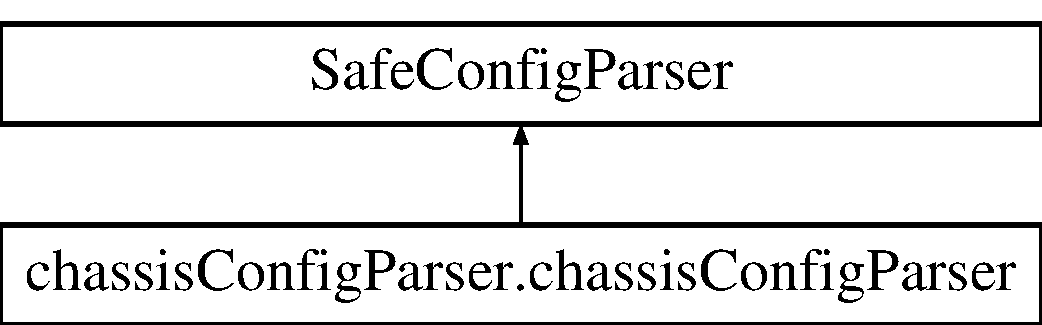
\includegraphics[height=2.000000cm]{classchassis_config_parser_1_1chassis_config_parser}
\end{center}
\end{figure}
\subsection*{Public Member Functions}
\begin{DoxyCompactItemize}
\item 
def \hyperlink{classchassis_config_parser_1_1chassis_config_parser_a1fdd2c5c9fbfc502390614248b193e40}{write}
\begin{DoxyCompactList}\small\item\em The function writes and creates a configuration file based on the input parameters. \end{DoxyCompactList}\item 
def \hyperlink{classchassis_config_parser_1_1chassis_config_parser_acc82f6735d3d5ba0df16c7c79fcb8a2a}{create\-Default\-File}
\begin{DoxyCompactList}\small\item\em This function will create a default file with default values at the location specified by the file\-Path parameter. \end{DoxyCompactList}\item 
def \hyperlink{classchassis_config_parser_1_1chassis_config_parser_a0248d8a624225ec74154dea93a9d2e64}{read}
\begin{DoxyCompactList}\small\item\em This function will return the information read from the configuration file. \end{DoxyCompactList}\end{DoxyCompactItemize}


\subsection{Detailed Description}
This class can read and write a Waveform\-Chassis configuration file. 



\subsection{Member Function Documentation}
\hypertarget{classchassis_config_parser_1_1chassis_config_parser_acc82f6735d3d5ba0df16c7c79fcb8a2a}{\index{chassis\-Config\-Parser\-::chassis\-Config\-Parser@{chassis\-Config\-Parser\-::chassis\-Config\-Parser}!create\-Default\-File@{create\-Default\-File}}
\index{create\-Default\-File@{create\-Default\-File}!chassisConfigParser::chassisConfigParser@{chassis\-Config\-Parser\-::chassis\-Config\-Parser}}
\subsubsection[{create\-Default\-File}]{\setlength{\rightskip}{0pt plus 5cm}def chassis\-Config\-Parser.\-chassis\-Config\-Parser.\-create\-Default\-File (
\begin{DoxyParamCaption}
\item[{}]{self, }
\item[{}]{file\-Path}
\end{DoxyParamCaption}
)}}\label{classchassis_config_parser_1_1chassis_config_parser_acc82f6735d3d5ba0df16c7c79fcb8a2a}


This function will create a default file with default values at the location specified by the file\-Path parameter. 


\begin{DoxyParams}{Parameters}
{\em file\-Path} & The location of the file to be created. \\
\hline
\end{DoxyParams}
\hypertarget{classchassis_config_parser_1_1chassis_config_parser_a0248d8a624225ec74154dea93a9d2e64}{\index{chassis\-Config\-Parser\-::chassis\-Config\-Parser@{chassis\-Config\-Parser\-::chassis\-Config\-Parser}!read@{read}}
\index{read@{read}!chassisConfigParser::chassisConfigParser@{chassis\-Config\-Parser\-::chassis\-Config\-Parser}}
\subsubsection[{read}]{\setlength{\rightskip}{0pt plus 5cm}def chassis\-Config\-Parser.\-chassis\-Config\-Parser.\-read (
\begin{DoxyParamCaption}
\item[{}]{self, }
\item[{}]{file\-Path}
\end{DoxyParamCaption}
)}}\label{classchassis_config_parser_1_1chassis_config_parser_a0248d8a624225ec74154dea93a9d2e64}


This function will return the information read from the configuration file. 

\hypertarget{classchassis_config_parser_1_1chassis_config_parser_a1fdd2c5c9fbfc502390614248b193e40}{\index{chassis\-Config\-Parser\-::chassis\-Config\-Parser@{chassis\-Config\-Parser\-::chassis\-Config\-Parser}!write@{write}}
\index{write@{write}!chassisConfigParser::chassisConfigParser@{chassis\-Config\-Parser\-::chassis\-Config\-Parser}}
\subsubsection[{write}]{\setlength{\rightskip}{0pt plus 5cm}def chassis\-Config\-Parser.\-chassis\-Config\-Parser.\-write (
\begin{DoxyParamCaption}
\item[{}]{self, }
\item[{}]{file\-Path, }
\item[{}]{data, }
\item[{}]{ni\-Sync\-Dev}
\end{DoxyParamCaption}
)}}\label{classchassis_config_parser_1_1chassis_config_parser_a1fdd2c5c9fbfc502390614248b193e40}


The function writes and creates a configuration file based on the input parameters. 


\begin{DoxyParams}{Parameters}
{\em self} & The object pointer. \\
\hline
{\em file\-Path} & The location of the file to be created \\
\hline
{\em data} & A dictionary containing the analog output and digital output channel names. \\
\hline
{\em ni\-Sync\-Dev} & The name of the N\-I-\/\-Sync card. \\
\hline
\end{DoxyParams}


The documentation for this class was generated from the following file\-:\begin{DoxyCompactItemize}
\item 
chassis\-Config\-Parser.\-py\end{DoxyCompactItemize}

\hypertarget{class_digital_output_1_1_digital_output}{\section{Digital\-Output.\-Digital\-Output Class Reference}
\label{class_digital_output_1_1_digital_output}\index{Digital\-Output.\-Digital\-Output@{Digital\-Output.\-Digital\-Output}}
}


This class will generate digital outputs using py\-D\-A\-Qmx.  


Inheritance diagram for Digital\-Output.\-Digital\-Output\-:\begin{figure}[H]
\begin{center}
\leavevmode
\includegraphics[height=2.000000cm]{class_digital_output_1_1_digital_output}
\end{center}
\end{figure}
\subsection*{Public Member Functions}
\begin{DoxyCompactItemize}
\item 
def \hyperlink{class_digital_output_1_1_digital_output_a0c8ab0946897540122502804d4b1a0eb}{get\-Sample\-Rate}
\begin{DoxyCompactList}\small\item\em This function returns the sample rate configured in the D\-A\-Qmx Task. \end{DoxyCompactList}\item 
def \hyperlink{class_digital_output_1_1_digital_output_a96ff9f9cb2f61ec977e9c6df2b525499}{set\-Sample\-Rate}
\begin{DoxyCompactList}\small\item\em This function sets the sample rate in the D\-A\-Qmx Task. \end{DoxyCompactList}\item 
def \hyperlink{class_digital_output_1_1_digital_output_aeef526fd09b2d6cc25c034a01bf16b0e}{get\-Samples\-Per\-Channel}
\begin{DoxyCompactList}\small\item\em This function returns the samples per channel configured in the D\-A\-Qmx Task. \end{DoxyCompactList}\item 
def \hyperlink{class_digital_output_1_1_digital_output_a7866f0194c502d7d99130513aafddb51}{set\-Samples\-Per\-Channel}
\begin{DoxyCompactList}\small\item\em This function sets the samples per channel in the D\-A\-Qmx Task. \end{DoxyCompactList}\item 
def \hyperlink{class_digital_output_1_1_digital_output_ac1122c27d8cacd4f4d7f3068d0613635}{get\-Clk\-Source}
\begin{DoxyCompactList}\small\item\em This function returns the sample clock source configured in the D\-A\-Qmx Task. \end{DoxyCompactList}\item 
def \hyperlink{class_digital_output_1_1_digital_output_a467edd75df46b381036ce37ca665e047}{set\-Clk\-Source}
\begin{DoxyCompactList}\small\item\em This function sets the sample clock source in the D\-A\-Qmx Task. \end{DoxyCompactList}\item 
def \hyperlink{class_digital_output_1_1_digital_output_a481e24aa22a2a7d516dd79e3460eb8dd}{\-\_\-\-\_\-init\-\_\-\-\_\-}
\begin{DoxyCompactList}\small\item\em This function is a constructor for the \hyperlink{class_digital_output_1_1_digital_output}{Digital\-Output} class. \end{DoxyCompactList}\item 
def \hyperlink{class_digital_output_1_1_digital_output_a35dd7e77a58e88f8cc0d02aaede8d6b0}{init}
\begin{DoxyCompactList}\small\item\em Initialize the digital outputs based on the object's configuration. \end{DoxyCompactList}\item 
def \hyperlink{class_digital_output_1_1_digital_output_aa888e91f47efed1049fd310373bd4fc9}{create\-Test\-Buffer}
\begin{DoxyCompactList}\small\item\em This function returns a random 1\-D numpy array of samples for writing the buffer of digital output channels. \end{DoxyCompactList}\item 
def \hyperlink{class_digital_output_1_1_digital_output_a0f143fe8af789b6623c3c9f4428c8514}{get\-Num\-Lines}
\begin{DoxyCompactList}\small\item\em This function returns the number of digital lines configured in the D\-A\-Qmx Task. \end{DoxyCompactList}\item 
def \hyperlink{class_digital_output_1_1_digital_output_a30a645662a4b0baa31990ed244cd91cc}{get\-Num\-Channels}
\begin{DoxyCompactList}\small\item\em This function returns the number of digital channels configured in the D\-A\-Qmx Task. \end{DoxyCompactList}\item 
def \hyperlink{class_digital_output_1_1_digital_output_a74440e738ee87a0b70a8388acba28c11}{write\-To\-Buffer}
\begin{DoxyCompactList}\small\item\em This function writes the specified values into the buffer. \end{DoxyCompactList}\item 
def \hyperlink{class_digital_output_1_1_digital_output_aff1c266b07a91eb42a96f4d394405d6b}{start}
\begin{DoxyCompactList}\small\item\em This function starts the digital output generation. \end{DoxyCompactList}\item 
def \hyperlink{class_digital_output_1_1_digital_output_a6a179ee4c172d0c99d20267d34437ad1}{wait\-Until\-Done}
\begin{DoxyCompactList}\small\item\em This functions waits for the digital output generation to complete. \end{DoxyCompactList}\item 
def \hyperlink{class_digital_output_1_1_digital_output_a7f5784b1fdea30aaddc1d608357accf1}{stop}
\begin{DoxyCompactList}\small\item\em This function stops the digital output generation. \end{DoxyCompactList}\item 
def \hyperlink{class_digital_output_1_1_digital_output_a5385404bf2191f7f6b23a30041599bab}{close}
\begin{DoxyCompactList}\small\item\em This function will close connection to the digital ouput device and channels. \end{DoxyCompactList}\item 
def \hyperlink{class_digital_output_1_1_digital_output_a4aea66b269b7202475ace284a26b87be}{\-\_\-\-\_\-del\-\_\-\-\_\-}
\begin{DoxyCompactList}\small\item\em This is the destructor for the \hyperlink{class_digital_output_1_1_digital_output}{Digital\-Output} Class. \end{DoxyCompactList}\end{DoxyCompactItemize}
\subsection*{Public Attributes}
\begin{DoxyCompactItemize}
\item 
\hyperlink{class_digital_output_1_1_digital_output_ad4c856a2b8d101078add570f1a5843a3}{status}
\begin{DoxyCompactList}\small\item\em This is the status of the D\-A\-Qmx task. \end{DoxyCompactList}\item 
\hyperlink{class_digital_output_1_1_digital_output_a2aeeacbf158f4acfdcb0461327396d98}{task\-Ref}
\begin{DoxyCompactList}\small\item\em The D\-A\-Qmx task reference. \end{DoxyCompactList}\item 
\hyperlink{class_digital_output_1_1_digital_output_af5c9fe7d592b5bcbd98ce90afc678fdc}{initialized}
\begin{DoxyCompactList}\small\item\em This is a boolean that is true when the D\-A\-Qmx task has been initialized. \end{DoxyCompactList}\item 
\hyperlink{class_digital_output_1_1_digital_output_a68b531bfedc4aa2fd7e54c24d2b9758e}{mode}
\begin{DoxyCompactList}\small\item\em This is the mode of operation for the digital outputs. \end{DoxyCompactList}\item 
\hyperlink{class_digital_output_1_1_digital_output_a352162e0da3e40979267c4263b726ead}{loops}
\begin{DoxyCompactList}\small\item\em The number of time to iterate over a Finite number of samples. \end{DoxyCompactList}\end{DoxyCompactItemize}
\subsection*{Properties}
\begin{DoxyCompactItemize}
\item 
\hyperlink{class_digital_output_1_1_digital_output_a3c7b4cb824baa168977ef85dbbc4d1d5}{sample\-Rate}
\begin{DoxyCompactList}\small\item\em This is the sample rate of the digital output. \end{DoxyCompactList}\item 
\hyperlink{class_digital_output_1_1_digital_output_a8de6ce12b96449fe3546d29d67bf1308}{samples\-Per\-Channel}
\begin{DoxyCompactList}\small\item\em This is the number of samples per channel that will be generated in Finite mode. \end{DoxyCompactList}\item 
\hyperlink{class_digital_output_1_1_digital_output_ac666f33f58ca6f93d9aaeb93f917e81c}{clk\-Source}
\begin{DoxyCompactList}\small\item\em This is the sample clock source terminal. \end{DoxyCompactList}\end{DoxyCompactItemize}


\subsection{Detailed Description}
This class will generate digital outputs using py\-D\-A\-Qmx. 



\subsection{Constructor \& Destructor Documentation}
\hypertarget{class_digital_output_1_1_digital_output_a481e24aa22a2a7d516dd79e3460eb8dd}{\index{Digital\-Output\-::\-Digital\-Output@{Digital\-Output\-::\-Digital\-Output}!\-\_\-\-\_\-init\-\_\-\-\_\-@{\-\_\-\-\_\-init\-\_\-\-\_\-}}
\index{\-\_\-\-\_\-init\-\_\-\-\_\-@{\-\_\-\-\_\-init\-\_\-\-\_\-}!DigitalOutput::DigitalOutput@{Digital\-Output\-::\-Digital\-Output}}
\subsubsection[{\-\_\-\-\_\-init\-\_\-\-\_\-}]{\setlength{\rightskip}{0pt plus 5cm}def Digital\-Output.\-Digital\-Output.\-\_\-\-\_\-init\-\_\-\-\_\- (
\begin{DoxyParamCaption}
\item[{}]{self}
\end{DoxyParamCaption}
)}}\label{class_digital_output_1_1_digital_output_a481e24aa22a2a7d516dd79e3460eb8dd}


This function is a constructor for the \hyperlink{class_digital_output_1_1_digital_output}{Digital\-Output} class. 

It creates the internal variables required to perform functions within the class. This function does not initialize any hardware. 
\begin{DoxyParams}{Parameters}
{\em self} & This object pointer \\
\hline
\end{DoxyParams}
\hypertarget{class_digital_output_1_1_digital_output_a4aea66b269b7202475ace284a26b87be}{\index{Digital\-Output\-::\-Digital\-Output@{Digital\-Output\-::\-Digital\-Output}!\-\_\-\-\_\-del\-\_\-\-\_\-@{\-\_\-\-\_\-del\-\_\-\-\_\-}}
\index{\-\_\-\-\_\-del\-\_\-\-\_\-@{\-\_\-\-\_\-del\-\_\-\-\_\-}!DigitalOutput::DigitalOutput@{Digital\-Output\-::\-Digital\-Output}}
\subsubsection[{\-\_\-\-\_\-del\-\_\-\-\_\-}]{\setlength{\rightskip}{0pt plus 5cm}def Digital\-Output.\-Digital\-Output.\-\_\-\-\_\-del\-\_\-\-\_\- (
\begin{DoxyParamCaption}
\item[{}]{self}
\end{DoxyParamCaption}
)}}\label{class_digital_output_1_1_digital_output_a4aea66b269b7202475ace284a26b87be}


This is the destructor for the \hyperlink{class_digital_output_1_1_digital_output}{Digital\-Output} Class. 


\begin{DoxyParams}{Parameters}
{\em self} & The object pointer. \\
\hline
\end{DoxyParams}


\subsection{Member Function Documentation}
\hypertarget{class_digital_output_1_1_digital_output_a5385404bf2191f7f6b23a30041599bab}{\index{Digital\-Output\-::\-Digital\-Output@{Digital\-Output\-::\-Digital\-Output}!close@{close}}
\index{close@{close}!DigitalOutput::DigitalOutput@{Digital\-Output\-::\-Digital\-Output}}
\subsubsection[{close}]{\setlength{\rightskip}{0pt plus 5cm}def Digital\-Output.\-Digital\-Output.\-close (
\begin{DoxyParamCaption}
\item[{}]{self}
\end{DoxyParamCaption}
)}}\label{class_digital_output_1_1_digital_output_a5385404bf2191f7f6b23a30041599bab}


This function will close connection to the digital ouput device and channels. 


\begin{DoxyParams}{Parameters}
{\em self} & The object pointer. \begin{DoxyVerb}\end{DoxyVerb}
 \\
\hline
\end{DoxyParams}
\hypertarget{class_digital_output_1_1_digital_output_aa888e91f47efed1049fd310373bd4fc9}{\index{Digital\-Output\-::\-Digital\-Output@{Digital\-Output\-::\-Digital\-Output}!create\-Test\-Buffer@{create\-Test\-Buffer}}
\index{create\-Test\-Buffer@{create\-Test\-Buffer}!DigitalOutput::DigitalOutput@{Digital\-Output\-::\-Digital\-Output}}
\subsubsection[{create\-Test\-Buffer}]{\setlength{\rightskip}{0pt plus 5cm}def Digital\-Output.\-Digital\-Output.\-create\-Test\-Buffer (
\begin{DoxyParamCaption}
\item[{}]{self}
\end{DoxyParamCaption}
)}}\label{class_digital_output_1_1_digital_output_aa888e91f47efed1049fd310373bd4fc9}


This function returns a random 1\-D numpy array of samples for writing the buffer of digital output channels. 


\begin{DoxyParams}{Parameters}
{\em self} & The objet pointer. \\
\hline
\end{DoxyParams}
\hypertarget{class_digital_output_1_1_digital_output_ac1122c27d8cacd4f4d7f3068d0613635}{\index{Digital\-Output\-::\-Digital\-Output@{Digital\-Output\-::\-Digital\-Output}!get\-Clk\-Source@{get\-Clk\-Source}}
\index{get\-Clk\-Source@{get\-Clk\-Source}!DigitalOutput::DigitalOutput@{Digital\-Output\-::\-Digital\-Output}}
\subsubsection[{get\-Clk\-Source}]{\setlength{\rightskip}{0pt plus 5cm}def Digital\-Output.\-Digital\-Output.\-get\-Clk\-Source (
\begin{DoxyParamCaption}
\item[{}]{self}
\end{DoxyParamCaption}
)}}\label{class_digital_output_1_1_digital_output_ac1122c27d8cacd4f4d7f3068d0613635}


This function returns the sample clock source configured in the D\-A\-Qmx Task. 


\begin{DoxyParams}{Parameters}
{\em self} & The object pointer. \\
\hline
\end{DoxyParams}
\hypertarget{class_digital_output_1_1_digital_output_a30a645662a4b0baa31990ed244cd91cc}{\index{Digital\-Output\-::\-Digital\-Output@{Digital\-Output\-::\-Digital\-Output}!get\-Num\-Channels@{get\-Num\-Channels}}
\index{get\-Num\-Channels@{get\-Num\-Channels}!DigitalOutput::DigitalOutput@{Digital\-Output\-::\-Digital\-Output}}
\subsubsection[{get\-Num\-Channels}]{\setlength{\rightskip}{0pt plus 5cm}def Digital\-Output.\-Digital\-Output.\-get\-Num\-Channels (
\begin{DoxyParamCaption}
\item[{}]{self}
\end{DoxyParamCaption}
)}}\label{class_digital_output_1_1_digital_output_a30a645662a4b0baa31990ed244cd91cc}


This function returns the number of digital channels configured in the D\-A\-Qmx Task. 


\begin{DoxyParams}{Parameters}
{\em self} & The object pointer. \\
\hline
\end{DoxyParams}
\hypertarget{class_digital_output_1_1_digital_output_a0f143fe8af789b6623c3c9f4428c8514}{\index{Digital\-Output\-::\-Digital\-Output@{Digital\-Output\-::\-Digital\-Output}!get\-Num\-Lines@{get\-Num\-Lines}}
\index{get\-Num\-Lines@{get\-Num\-Lines}!DigitalOutput::DigitalOutput@{Digital\-Output\-::\-Digital\-Output}}
\subsubsection[{get\-Num\-Lines}]{\setlength{\rightskip}{0pt plus 5cm}def Digital\-Output.\-Digital\-Output.\-get\-Num\-Lines (
\begin{DoxyParamCaption}
\item[{}]{self}
\end{DoxyParamCaption}
)}}\label{class_digital_output_1_1_digital_output_a0f143fe8af789b6623c3c9f4428c8514}


This function returns the number of digital lines configured in the D\-A\-Qmx Task. 


\begin{DoxyParams}{Parameters}
{\em self} & The object pointer. \\
\hline
\end{DoxyParams}
\hypertarget{class_digital_output_1_1_digital_output_a0c8ab0946897540122502804d4b1a0eb}{\index{Digital\-Output\-::\-Digital\-Output@{Digital\-Output\-::\-Digital\-Output}!get\-Sample\-Rate@{get\-Sample\-Rate}}
\index{get\-Sample\-Rate@{get\-Sample\-Rate}!DigitalOutput::DigitalOutput@{Digital\-Output\-::\-Digital\-Output}}
\subsubsection[{get\-Sample\-Rate}]{\setlength{\rightskip}{0pt plus 5cm}def Digital\-Output.\-Digital\-Output.\-get\-Sample\-Rate (
\begin{DoxyParamCaption}
\item[{}]{self}
\end{DoxyParamCaption}
)}}\label{class_digital_output_1_1_digital_output_a0c8ab0946897540122502804d4b1a0eb}


This function returns the sample rate configured in the D\-A\-Qmx Task. 


\begin{DoxyParams}{Parameters}
{\em self} & The object pointer. \\
\hline
\end{DoxyParams}
\hypertarget{class_digital_output_1_1_digital_output_aeef526fd09b2d6cc25c034a01bf16b0e}{\index{Digital\-Output\-::\-Digital\-Output@{Digital\-Output\-::\-Digital\-Output}!get\-Samples\-Per\-Channel@{get\-Samples\-Per\-Channel}}
\index{get\-Samples\-Per\-Channel@{get\-Samples\-Per\-Channel}!DigitalOutput::DigitalOutput@{Digital\-Output\-::\-Digital\-Output}}
\subsubsection[{get\-Samples\-Per\-Channel}]{\setlength{\rightskip}{0pt plus 5cm}def Digital\-Output.\-Digital\-Output.\-get\-Samples\-Per\-Channel (
\begin{DoxyParamCaption}
\item[{}]{self}
\end{DoxyParamCaption}
)}}\label{class_digital_output_1_1_digital_output_aeef526fd09b2d6cc25c034a01bf16b0e}


This function returns the samples per channel configured in the D\-A\-Qmx Task. 


\begin{DoxyParams}{Parameters}
{\em self} & The object pointer. \\
\hline
\end{DoxyParams}
\hypertarget{class_digital_output_1_1_digital_output_a35dd7e77a58e88f8cc0d02aaede8d6b0}{\index{Digital\-Output\-::\-Digital\-Output@{Digital\-Output\-::\-Digital\-Output}!init@{init}}
\index{init@{init}!DigitalOutput::DigitalOutput@{Digital\-Output\-::\-Digital\-Output}}
\subsubsection[{init}]{\setlength{\rightskip}{0pt plus 5cm}def Digital\-Output.\-Digital\-Output.\-init (
\begin{DoxyParamCaption}
\item[{}]{self, }
\item[{}]{physical\-Channel}
\end{DoxyParamCaption}
)}}\label{class_digital_output_1_1_digital_output_a35dd7e77a58e88f8cc0d02aaede8d6b0}


Initialize the digital outputs based on the object's configuration. 


\begin{DoxyParams}{Parameters}
{\em self} & The object pointer. \\
\hline
{\em physical\-Channel} & A string representing the device and digital output channels. Example value\-: \char`\"{}\-P\-X\-I1\-Slot3/ao0\-:7\char`\"{} \\
\hline
\end{DoxyParams}
\hypertarget{class_digital_output_1_1_digital_output_a467edd75df46b381036ce37ca665e047}{\index{Digital\-Output\-::\-Digital\-Output@{Digital\-Output\-::\-Digital\-Output}!set\-Clk\-Source@{set\-Clk\-Source}}
\index{set\-Clk\-Source@{set\-Clk\-Source}!DigitalOutput::DigitalOutput@{Digital\-Output\-::\-Digital\-Output}}
\subsubsection[{set\-Clk\-Source}]{\setlength{\rightskip}{0pt plus 5cm}def Digital\-Output.\-Digital\-Output.\-set\-Clk\-Source (
\begin{DoxyParamCaption}
\item[{}]{self, }
\item[{}]{value}
\end{DoxyParamCaption}
)}}\label{class_digital_output_1_1_digital_output_a467edd75df46b381036ce37ca665e047}


This function sets the sample clock source in the D\-A\-Qmx Task. 


\begin{DoxyParams}{Parameters}
{\em self} & The object pointer. \\
\hline
{\em value} & The value to set the clock source. \\
\hline
\end{DoxyParams}
\hypertarget{class_digital_output_1_1_digital_output_a96ff9f9cb2f61ec977e9c6df2b525499}{\index{Digital\-Output\-::\-Digital\-Output@{Digital\-Output\-::\-Digital\-Output}!set\-Sample\-Rate@{set\-Sample\-Rate}}
\index{set\-Sample\-Rate@{set\-Sample\-Rate}!DigitalOutput::DigitalOutput@{Digital\-Output\-::\-Digital\-Output}}
\subsubsection[{set\-Sample\-Rate}]{\setlength{\rightskip}{0pt plus 5cm}def Digital\-Output.\-Digital\-Output.\-set\-Sample\-Rate (
\begin{DoxyParamCaption}
\item[{}]{self, }
\item[{}]{value}
\end{DoxyParamCaption}
)}}\label{class_digital_output_1_1_digital_output_a96ff9f9cb2f61ec977e9c6df2b525499}


This function sets the sample rate in the D\-A\-Qmx Task. 


\begin{DoxyParams}{Parameters}
{\em self} & The object pointer. \\
\hline
{\em value} & The value to set the sample rate. \\
\hline
\end{DoxyParams}
\hypertarget{class_digital_output_1_1_digital_output_a7866f0194c502d7d99130513aafddb51}{\index{Digital\-Output\-::\-Digital\-Output@{Digital\-Output\-::\-Digital\-Output}!set\-Samples\-Per\-Channel@{set\-Samples\-Per\-Channel}}
\index{set\-Samples\-Per\-Channel@{set\-Samples\-Per\-Channel}!DigitalOutput::DigitalOutput@{Digital\-Output\-::\-Digital\-Output}}
\subsubsection[{set\-Samples\-Per\-Channel}]{\setlength{\rightskip}{0pt plus 5cm}def Digital\-Output.\-Digital\-Output.\-set\-Samples\-Per\-Channel (
\begin{DoxyParamCaption}
\item[{}]{self, }
\item[{}]{value}
\end{DoxyParamCaption}
)}}\label{class_digital_output_1_1_digital_output_a7866f0194c502d7d99130513aafddb51}


This function sets the samples per channel in the D\-A\-Qmx Task. 


\begin{DoxyParams}{Parameters}
{\em self} & The object pointer. \\
\hline
{\em value} & The value to set the samples per channel. \\
\hline
\end{DoxyParams}
\hypertarget{class_digital_output_1_1_digital_output_aff1c266b07a91eb42a96f4d394405d6b}{\index{Digital\-Output\-::\-Digital\-Output@{Digital\-Output\-::\-Digital\-Output}!start@{start}}
\index{start@{start}!DigitalOutput::DigitalOutput@{Digital\-Output\-::\-Digital\-Output}}
\subsubsection[{start}]{\setlength{\rightskip}{0pt plus 5cm}def Digital\-Output.\-Digital\-Output.\-start (
\begin{DoxyParamCaption}
\item[{}]{self}
\end{DoxyParamCaption}
)}}\label{class_digital_output_1_1_digital_output_aff1c266b07a91eb42a96f4d394405d6b}


This function starts the digital output generation. 


\begin{DoxyParams}{Parameters}
{\em self} & The object pointer. \\
\hline
\end{DoxyParams}
\hypertarget{class_digital_output_1_1_digital_output_a7f5784b1fdea30aaddc1d608357accf1}{\index{Digital\-Output\-::\-Digital\-Output@{Digital\-Output\-::\-Digital\-Output}!stop@{stop}}
\index{stop@{stop}!DigitalOutput::DigitalOutput@{Digital\-Output\-::\-Digital\-Output}}
\subsubsection[{stop}]{\setlength{\rightskip}{0pt plus 5cm}def Digital\-Output.\-Digital\-Output.\-stop (
\begin{DoxyParamCaption}
\item[{}]{self}
\end{DoxyParamCaption}
)}}\label{class_digital_output_1_1_digital_output_a7f5784b1fdea30aaddc1d608357accf1}


This function stops the digital output generation. 


\begin{DoxyParams}{Parameters}
{\em self} & The object pointer. \\
\hline
\end{DoxyParams}
\hypertarget{class_digital_output_1_1_digital_output_a6a179ee4c172d0c99d20267d34437ad1}{\index{Digital\-Output\-::\-Digital\-Output@{Digital\-Output\-::\-Digital\-Output}!wait\-Until\-Done@{wait\-Until\-Done}}
\index{wait\-Until\-Done@{wait\-Until\-Done}!DigitalOutput::DigitalOutput@{Digital\-Output\-::\-Digital\-Output}}
\subsubsection[{wait\-Until\-Done}]{\setlength{\rightskip}{0pt plus 5cm}def Digital\-Output.\-Digital\-Output.\-wait\-Until\-Done (
\begin{DoxyParamCaption}
\item[{}]{self}
\end{DoxyParamCaption}
)}}\label{class_digital_output_1_1_digital_output_a6a179ee4c172d0c99d20267d34437ad1}


This functions waits for the digital output generation to complete. 


\begin{DoxyParams}{Parameters}
{\em self} & The object pointer. \\
\hline
\end{DoxyParams}
\hypertarget{class_digital_output_1_1_digital_output_a74440e738ee87a0b70a8388acba28c11}{\index{Digital\-Output\-::\-Digital\-Output@{Digital\-Output\-::\-Digital\-Output}!write\-To\-Buffer@{write\-To\-Buffer}}
\index{write\-To\-Buffer@{write\-To\-Buffer}!DigitalOutput::DigitalOutput@{Digital\-Output\-::\-Digital\-Output}}
\subsubsection[{write\-To\-Buffer}]{\setlength{\rightskip}{0pt plus 5cm}def Digital\-Output.\-Digital\-Output.\-write\-To\-Buffer (
\begin{DoxyParamCaption}
\item[{}]{self, }
\item[{}]{data}
\end{DoxyParamCaption}
)}}\label{class_digital_output_1_1_digital_output_a74440e738ee87a0b70a8388acba28c11}


This function writes the specified values into the buffer. 


\begin{DoxyParams}{Parameters}
{\em self} & The object pointer. \\
\hline
{\em data} & This is a 1\-D 8-\/bit unsigned integer array that contians samples for each digital channel. Channels are non-\/interleaved (channel1 n-\/samples then channel2 n-\/samples). \\
\hline
\end{DoxyParams}


\subsection{Member Data Documentation}
\hypertarget{class_digital_output_1_1_digital_output_af5c9fe7d592b5bcbd98ce90afc678fdc}{\index{Digital\-Output\-::\-Digital\-Output@{Digital\-Output\-::\-Digital\-Output}!initialized@{initialized}}
\index{initialized@{initialized}!DigitalOutput::DigitalOutput@{Digital\-Output\-::\-Digital\-Output}}
\subsubsection[{initialized}]{\setlength{\rightskip}{0pt plus 5cm}Digital\-Output.\-Digital\-Output.\-initialized}}\label{class_digital_output_1_1_digital_output_af5c9fe7d592b5bcbd98ce90afc678fdc}


This is a boolean that is true when the D\-A\-Qmx task has been initialized. 

\hypertarget{class_digital_output_1_1_digital_output_a352162e0da3e40979267c4263b726ead}{\index{Digital\-Output\-::\-Digital\-Output@{Digital\-Output\-::\-Digital\-Output}!loops@{loops}}
\index{loops@{loops}!DigitalOutput::DigitalOutput@{Digital\-Output\-::\-Digital\-Output}}
\subsubsection[{loops}]{\setlength{\rightskip}{0pt plus 5cm}Digital\-Output.\-Digital\-Output.\-loops}}\label{class_digital_output_1_1_digital_output_a352162e0da3e40979267c4263b726ead}


The number of time to iterate over a Finite number of samples. 

This value is only useful in the \char`\"{}\-Finite\char`\"{} mode. It is the number of times that a sequence of digital samples will be looped. The default is allways 1. \hypertarget{class_digital_output_1_1_digital_output_a68b531bfedc4aa2fd7e54c24d2b9758e}{\index{Digital\-Output\-::\-Digital\-Output@{Digital\-Output\-::\-Digital\-Output}!mode@{mode}}
\index{mode@{mode}!DigitalOutput::DigitalOutput@{Digital\-Output\-::\-Digital\-Output}}
\subsubsection[{mode}]{\setlength{\rightskip}{0pt plus 5cm}Digital\-Output.\-Digital\-Output.\-mode}}\label{class_digital_output_1_1_digital_output_a68b531bfedc4aa2fd7e54c24d2b9758e}


This is the mode of operation for the digital outputs. 

There are currently three modes available. Static mode is where one static digital sample is set with no need for a sample clock. Finite mode is where a finite number of digital samples will be set at a sample clock rate. Continuous mode is where a sequence of voltages are generated at a sample rate and then repeated until the \hyperlink{class_digital_output_1_1_digital_output_a7f5784b1fdea30aaddc1d608357accf1}{stop()} method is called. \hypertarget{class_digital_output_1_1_digital_output_ad4c856a2b8d101078add570f1a5843a3}{\index{Digital\-Output\-::\-Digital\-Output@{Digital\-Output\-::\-Digital\-Output}!status@{status}}
\index{status@{status}!DigitalOutput::DigitalOutput@{Digital\-Output\-::\-Digital\-Output}}
\subsubsection[{status}]{\setlength{\rightskip}{0pt plus 5cm}Digital\-Output.\-Digital\-Output.\-status}}\label{class_digital_output_1_1_digital_output_ad4c856a2b8d101078add570f1a5843a3}


This is the status of the D\-A\-Qmx task. 

A value greater than 0 means that an error has occurred. When the status is greater than 0 an error should be reported by the class. \hypertarget{class_digital_output_1_1_digital_output_a2aeeacbf158f4acfdcb0461327396d98}{\index{Digital\-Output\-::\-Digital\-Output@{Digital\-Output\-::\-Digital\-Output}!task\-Ref@{task\-Ref}}
\index{task\-Ref@{task\-Ref}!DigitalOutput::DigitalOutput@{Digital\-Output\-::\-Digital\-Output}}
\subsubsection[{task\-Ref}]{\setlength{\rightskip}{0pt plus 5cm}Digital\-Output.\-Digital\-Output.\-task\-Ref}}\label{class_digital_output_1_1_digital_output_a2aeeacbf158f4acfdcb0461327396d98}


The D\-A\-Qmx task reference. 



\subsection{Property Documentation}
\hypertarget{class_digital_output_1_1_digital_output_ac666f33f58ca6f93d9aaeb93f917e81c}{\index{Digital\-Output\-::\-Digital\-Output@{Digital\-Output\-::\-Digital\-Output}!clk\-Source@{clk\-Source}}
\index{clk\-Source@{clk\-Source}!DigitalOutput::DigitalOutput@{Digital\-Output\-::\-Digital\-Output}}
\subsubsection[{clk\-Source}]{\setlength{\rightskip}{0pt plus 5cm}Digital\-Output.\-Digital\-Output.\-clk\-Source\hspace{0.3cm}{\ttfamily [static]}}}\label{class_digital_output_1_1_digital_output_ac666f33f58ca6f93d9aaeb93f917e81c}
{\bfseries Initial value\-:}
\begin{DoxyCode}
1 property(getClkSource, setClkSource, \_delClkSource,
2     \textcolor{stringliteral}{"""The clock source for the digital outputsample clock."""})
\end{DoxyCode}


This is the sample clock source terminal. 

It can be set to an internal clock or external clock such as a P\-F\-I line i.\-e. \char`\"{}/\-P\-X\-I1\-Slot3/\-P\-F\-I15.\char`\"{} \hypertarget{class_digital_output_1_1_digital_output_a3c7b4cb824baa168977ef85dbbc4d1d5}{\index{Digital\-Output\-::\-Digital\-Output@{Digital\-Output\-::\-Digital\-Output}!sample\-Rate@{sample\-Rate}}
\index{sample\-Rate@{sample\-Rate}!DigitalOutput::DigitalOutput@{Digital\-Output\-::\-Digital\-Output}}
\subsubsection[{sample\-Rate}]{\setlength{\rightskip}{0pt plus 5cm}Digital\-Output.\-Digital\-Output.\-sample\-Rate\hspace{0.3cm}{\ttfamily [static]}}}\label{class_digital_output_1_1_digital_output_a3c7b4cb824baa168977ef85dbbc4d1d5}
{\bfseries Initial value\-:}
\begin{DoxyCode}
1 property(getSampleRate, setSampleRate, \_delSampleRate, doc=
2                              \textcolor{stringliteral}{"""The sample rate of the digital output."""})
\end{DoxyCode}


This is the sample rate of the digital output. 

\hypertarget{class_digital_output_1_1_digital_output_a8de6ce12b96449fe3546d29d67bf1308}{\index{Digital\-Output\-::\-Digital\-Output@{Digital\-Output\-::\-Digital\-Output}!samples\-Per\-Channel@{samples\-Per\-Channel}}
\index{samples\-Per\-Channel@{samples\-Per\-Channel}!DigitalOutput::DigitalOutput@{Digital\-Output\-::\-Digital\-Output}}
\subsubsection[{samples\-Per\-Channel}]{\setlength{\rightskip}{0pt plus 5cm}Digital\-Output.\-Digital\-Output.\-samples\-Per\-Channel\hspace{0.3cm}{\ttfamily [static]}}}\label{class_digital_output_1_1_digital_output_a8de6ce12b96449fe3546d29d67bf1308}
{\bfseries Initial value\-:}
\begin{DoxyCode}
1 property(getSamplesPerChannel, setSamplesPerChannel,
2             \_delSamplesPerChannel,
3             \textcolor{stringliteral}{"""The samples per channel of the digital output."""})
\end{DoxyCode}


This is the number of samples per channel that will be generated in Finite mode. 



The documentation for this class was generated from the following file\-:\begin{DoxyCompactItemize}
\item 
Digital\-Output.\-py\end{DoxyCompactItemize}

\hypertarget{classe_map_parser_1_1e_map_parser}{\section{e\-Map\-Parser.\-e\-Map\-Parser Class Reference}
\label{classe_map_parser_1_1e_map_parser}\index{e\-Map\-Parser.\-e\-Map\-Parser@{e\-Map\-Parser.\-e\-Map\-Parser}}
}


This class will parse the electrode mape file.  


Inheritance diagram for e\-Map\-Parser.\-e\-Map\-Parser\-:\begin{figure}[H]
\begin{center}
\leavevmode
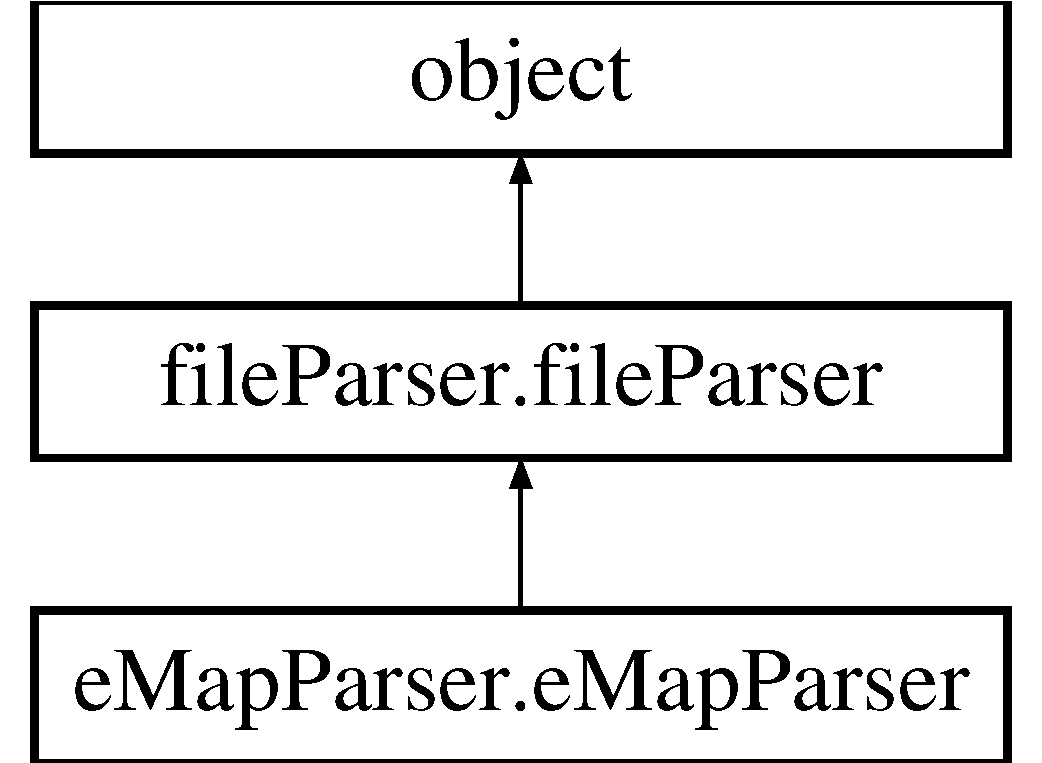
\includegraphics[height=3.000000cm]{classe_map_parser_1_1e_map_parser}
\end{center}
\end{figure}
\subsection*{Public Member Functions}
\begin{DoxyCompactItemize}
\item 
def \hyperlink{classe_map_parser_1_1e_map_parser_aa0199d0342cb5e5714ef75fbc0fcd857}{read}
\begin{DoxyCompactList}\small\item\em This function will read all of the data from the e\-Map file and return a list of electrodes, ao numbers, and dsub numbers. \end{DoxyCompactList}\end{DoxyCompactItemize}
\subsection*{Additional Inherited Members}


\subsection{Detailed Description}
This class will parse the electrode mape file. 



\subsection{Member Function Documentation}
\hypertarget{classe_map_parser_1_1e_map_parser_aa0199d0342cb5e5714ef75fbc0fcd857}{\index{e\-Map\-Parser\-::e\-Map\-Parser@{e\-Map\-Parser\-::e\-Map\-Parser}!read@{read}}
\index{read@{read}!eMapParser::eMapParser@{e\-Map\-Parser\-::e\-Map\-Parser}}
\subsubsection[{read}]{\setlength{\rightskip}{0pt plus 5cm}def e\-Map\-Parser.\-e\-Map\-Parser.\-read (
\begin{DoxyParamCaption}
\item[{}]{self}
\end{DoxyParamCaption}
)}}\label{classe_map_parser_1_1e_map_parser_aa0199d0342cb5e5714ef75fbc0fcd857}


This function will read all of the data from the e\-Map file and return a list of electrodes, ao numbers, and dsub numbers. 



The documentation for this class was generated from the following file\-:\begin{DoxyCompactItemize}
\item 
e\-Map\-Parser.\-py\end{DoxyCompactItemize}

\hypertarget{classfile_parser_1_1file_parser}{\section{file\-Parser.\-file\-Parser Class Reference}
\label{classfile_parser_1_1file_parser}\index{file\-Parser.\-file\-Parser@{file\-Parser.\-file\-Parser}}
}


This class is the parent class of all file parsers.  


Inheritance diagram for file\-Parser.\-file\-Parser\-:\begin{figure}[H]
\begin{center}
\leavevmode
\includegraphics[height=3.000000cm]{classfile_parser_1_1file_parser}
\end{center}
\end{figure}
\subsection*{Public Member Functions}
\begin{DoxyCompactItemize}
\item 
def \hyperlink{classfile_parser_1_1file_parser_a719b66d5fbb38b07112ac5770ee7227f}{\-\_\-\-\_\-init\-\_\-\-\_\-}
\begin{DoxyCompactList}\small\item\em This funciton is the constructor of the \hyperlink{classfile_parser_1_1file_parser}{file\-Parser} class. \end{DoxyCompactList}\item 
def \hyperlink{classfile_parser_1_1file_parser_ae60626fb0335d75b12a8dd80cc29db7e}{open}
\begin{DoxyCompactList}\small\item\em This function opens the file in the file\-Path argument. \end{DoxyCompactList}\item 
def \hyperlink{classfile_parser_1_1file_parser_a09b008848fe8dc2dcff9c59df98345d6}{get\-Num\-Lines}
\begin{DoxyCompactList}\small\item\em This function will return the number of lines within the file. \end{DoxyCompactList}\item 
def \hyperlink{classfile_parser_1_1file_parser_acbb2b6efa885326b69b165904ff2f8d2}{close}
\begin{DoxyCompactList}\small\item\em This function will close the file. \end{DoxyCompactList}\end{DoxyCompactItemize}
\subsection*{Public Attributes}
\begin{DoxyCompactItemize}
\item 
\hyperlink{classfile_parser_1_1file_parser_a7de27c6e6e7bc515c7909be87ea82dca}{file\-Obj}
\begin{DoxyCompactList}\small\item\em The file object for the file. \end{DoxyCompactList}\item 
\hyperlink{classfile_parser_1_1file_parser_a9531ba3360a53c234d49f24cc3c0d5cd}{comments}
\begin{DoxyCompactList}\small\item\em The comments within the file as a list. \end{DoxyCompactList}\item 
\hyperlink{classfile_parser_1_1file_parser_aa84b3558bdd36dbba71265753c4fb04f}{meta}
\begin{DoxyCompactList}\small\item\em The meta data of the file as a list. \end{DoxyCompactList}\item 
\hyperlink{classfile_parser_1_1file_parser_a8a31b5717e4f21af3f8b5f8d2f590310}{empty}
\begin{DoxyCompactList}\small\item\em A boolean value that is true if the file is empty, and false otherwise. \end{DoxyCompactList}\end{DoxyCompactItemize}
\subsection*{Properties}
\begin{DoxyCompactItemize}
\item 
\hyperlink{classfile_parser_1_1file_parser_ad7d86e199f948e8ce19303dc875bb32f}{total\-Lines}
\begin{DoxyCompactList}\small\item\em This is the total number of lines of data within the itf file. \end{DoxyCompactList}\end{DoxyCompactItemize}


\subsection{Detailed Description}
This class is the parent class of all file parsers. 



\subsection{Constructor \& Destructor Documentation}
\hypertarget{classfile_parser_1_1file_parser_a719b66d5fbb38b07112ac5770ee7227f}{\index{file\-Parser\-::file\-Parser@{file\-Parser\-::file\-Parser}!\-\_\-\-\_\-init\-\_\-\-\_\-@{\-\_\-\-\_\-init\-\_\-\-\_\-}}
\index{\-\_\-\-\_\-init\-\_\-\-\_\-@{\-\_\-\-\_\-init\-\_\-\-\_\-}!fileParser::fileParser@{file\-Parser\-::file\-Parser}}
\subsubsection[{\-\_\-\-\_\-init\-\_\-\-\_\-}]{\setlength{\rightskip}{0pt plus 5cm}def file\-Parser.\-file\-Parser.\-\_\-\-\_\-init\-\_\-\-\_\- (
\begin{DoxyParamCaption}
\item[{}]{self, }
\item[{}]{file\-Obj = {\ttfamily None}, }
\item[{}]{file\-Path = {\ttfamily None}}
\end{DoxyParamCaption}
)}}\label{classfile_parser_1_1file_parser_a719b66d5fbb38b07112ac5770ee7227f}


This funciton is the constructor of the \hyperlink{classfile_parser_1_1file_parser}{file\-Parser} class. 

It creates class data and opens the file if the file\-Path argument is provided. 
\begin{DoxyParams}{Parameters}
{\em self} & The object pointer. \\
\hline
{\em file\-Obj} & The file object that gets returned by the file \hyperlink{classfile_parser_1_1file_parser_ae60626fb0335d75b12a8dd80cc29db7e}{open()} function. \\
\hline
{\em file\-Path} & A string that represents the location of the file. \\
\hline
\end{DoxyParams}


\subsection{Member Function Documentation}
\hypertarget{classfile_parser_1_1file_parser_acbb2b6efa885326b69b165904ff2f8d2}{\index{file\-Parser\-::file\-Parser@{file\-Parser\-::file\-Parser}!close@{close}}
\index{close@{close}!fileParser::fileParser@{file\-Parser\-::file\-Parser}}
\subsubsection[{close}]{\setlength{\rightskip}{0pt plus 5cm}def file\-Parser.\-file\-Parser.\-close (
\begin{DoxyParamCaption}
\item[{}]{self}
\end{DoxyParamCaption}
)}}\label{classfile_parser_1_1file_parser_acbb2b6efa885326b69b165904ff2f8d2}


This function will close the file. 


\begin{DoxyParams}{Parameters}
{\em self} & The object pointer. \\
\hline
\end{DoxyParams}
\hypertarget{classfile_parser_1_1file_parser_a09b008848fe8dc2dcff9c59df98345d6}{\index{file\-Parser\-::file\-Parser@{file\-Parser\-::file\-Parser}!get\-Num\-Lines@{get\-Num\-Lines}}
\index{get\-Num\-Lines@{get\-Num\-Lines}!fileParser::fileParser@{file\-Parser\-::file\-Parser}}
\subsubsection[{get\-Num\-Lines}]{\setlength{\rightskip}{0pt plus 5cm}def file\-Parser.\-file\-Parser.\-get\-Num\-Lines (
\begin{DoxyParamCaption}
\item[{}]{self}
\end{DoxyParamCaption}
)}}\label{classfile_parser_1_1file_parser_a09b008848fe8dc2dcff9c59df98345d6}


This function will return the number of lines within the file. 

This function is equivalent to reading the total\-Lines variable within the class. 
\begin{DoxyParams}{Parameters}
{\em self} & The object pointer. \\
\hline
\end{DoxyParams}
\hypertarget{classfile_parser_1_1file_parser_ae60626fb0335d75b12a8dd80cc29db7e}{\index{file\-Parser\-::file\-Parser@{file\-Parser\-::file\-Parser}!open@{open}}
\index{open@{open}!fileParser::fileParser@{file\-Parser\-::file\-Parser}}
\subsubsection[{open}]{\setlength{\rightskip}{0pt plus 5cm}def file\-Parser.\-file\-Parser.\-open (
\begin{DoxyParamCaption}
\item[{}]{self, }
\item[{}]{file\-Path}
\end{DoxyParamCaption}
)}}\label{classfile_parser_1_1file_parser_ae60626fb0335d75b12a8dd80cc29db7e}


This function opens the file in the file\-Path argument. 


\begin{DoxyParams}{Parameters}
{\em self} & The object pointer. \\
\hline
{\em file\-Path} & This is the path to the file. \\
\hline
\end{DoxyParams}


\subsection{Member Data Documentation}
\hypertarget{classfile_parser_1_1file_parser_a9531ba3360a53c234d49f24cc3c0d5cd}{\index{file\-Parser\-::file\-Parser@{file\-Parser\-::file\-Parser}!comments@{comments}}
\index{comments@{comments}!fileParser::fileParser@{file\-Parser\-::file\-Parser}}
\subsubsection[{comments}]{\setlength{\rightskip}{0pt plus 5cm}file\-Parser.\-file\-Parser.\-comments}}\label{classfile_parser_1_1file_parser_a9531ba3360a53c234d49f24cc3c0d5cd}


The comments within the file as a list. 

\hypertarget{classfile_parser_1_1file_parser_a8a31b5717e4f21af3f8b5f8d2f590310}{\index{file\-Parser\-::file\-Parser@{file\-Parser\-::file\-Parser}!empty@{empty}}
\index{empty@{empty}!fileParser::fileParser@{file\-Parser\-::file\-Parser}}
\subsubsection[{empty}]{\setlength{\rightskip}{0pt plus 5cm}file\-Parser.\-file\-Parser.\-empty}}\label{classfile_parser_1_1file_parser_a8a31b5717e4f21af3f8b5f8d2f590310}


A boolean value that is true if the file is empty, and false otherwise. 

\hypertarget{classfile_parser_1_1file_parser_a7de27c6e6e7bc515c7909be87ea82dca}{\index{file\-Parser\-::file\-Parser@{file\-Parser\-::file\-Parser}!file\-Obj@{file\-Obj}}
\index{file\-Obj@{file\-Obj}!fileParser::fileParser@{file\-Parser\-::file\-Parser}}
\subsubsection[{file\-Obj}]{\setlength{\rightskip}{0pt plus 5cm}file\-Parser.\-file\-Parser.\-file\-Obj}}\label{classfile_parser_1_1file_parser_a7de27c6e6e7bc515c7909be87ea82dca}


The file object for the file. 

\hypertarget{classfile_parser_1_1file_parser_aa84b3558bdd36dbba71265753c4fb04f}{\index{file\-Parser\-::file\-Parser@{file\-Parser\-::file\-Parser}!meta@{meta}}
\index{meta@{meta}!fileParser::fileParser@{file\-Parser\-::file\-Parser}}
\subsubsection[{meta}]{\setlength{\rightskip}{0pt plus 5cm}file\-Parser.\-file\-Parser.\-meta}}\label{classfile_parser_1_1file_parser_aa84b3558bdd36dbba71265753c4fb04f}


The meta data of the file as a list. 

The dt variable is often within an itf file. The value of this variable will be a value within meta. 

\subsection{Property Documentation}
\hypertarget{classfile_parser_1_1file_parser_ad7d86e199f948e8ce19303dc875bb32f}{\index{file\-Parser\-::file\-Parser@{file\-Parser\-::file\-Parser}!total\-Lines@{total\-Lines}}
\index{total\-Lines@{total\-Lines}!fileParser::fileParser@{file\-Parser\-::file\-Parser}}
\subsubsection[{total\-Lines}]{\setlength{\rightskip}{0pt plus 5cm}file\-Parser.\-file\-Parser.\-total\-Lines\hspace{0.3cm}{\ttfamily [static]}}}\label{classfile_parser_1_1file_parser_ad7d86e199f948e8ce19303dc875bb32f}
{\bfseries Initial value\-:}
\begin{DoxyCode}
1 property(getNumLines,
2                doc = \textcolor{stringliteral}{"""The total number of lines in the file."""})
\end{DoxyCode}


This is the total number of lines of data within the itf file. 



The documentation for this class was generated from the following file\-:\begin{DoxyCompactItemize}
\item 
file\-Parser.\-py\end{DoxyCompactItemize}

\hypertarget{classfile_parser_1_1file_parser_error}{\section{file\-Parser.\-file\-Parser\-Error Class Reference}
\label{classfile_parser_1_1file_parser_error}\index{file\-Parser.\-file\-Parser\-Error@{file\-Parser.\-file\-Parser\-Error}}
}


This is a class that creates a specific exception for the \hyperlink{classfile_parser_1_1file_parser}{file\-Parser} class.  


Inheritance diagram for file\-Parser.\-file\-Parser\-Error\-:\begin{figure}[H]
\begin{center}
\leavevmode
\includegraphics[height=2.000000cm]{classfile_parser_1_1file_parser_error}
\end{center}
\end{figure}
\subsection*{Public Member Functions}
\begin{DoxyCompactItemize}
\item 
def \hyperlink{classfile_parser_1_1file_parser_error_aa3fbd8b07486310a324f24c7c11776cf}{\-\_\-\-\_\-init\-\_\-\-\_\-}
\begin{DoxyCompactList}\small\item\em This is the constructor for the \hyperlink{classfile_parser_1_1file_parser_error}{file\-Parser\-Error} class. \end{DoxyCompactList}\item 
def \hyperlink{classfile_parser_1_1file_parser_error_ab6f80a5cd6e1e0edc808b41df0c85d16}{\-\_\-\-\_\-str\-\_\-\-\_\-}
\begin{DoxyCompactList}\small\item\em This function defines how the class operates when a the class is asked to represent itself as a string. \end{DoxyCompactList}\end{DoxyCompactItemize}
\subsection*{Public Attributes}
\begin{DoxyCompactItemize}
\item 
\hyperlink{classfile_parser_1_1file_parser_error_a10a1298f8ac5493a909514edf50e26bc}{msg}
\begin{DoxyCompactList}\small\item\em The message to display to the user. \end{DoxyCompactList}\end{DoxyCompactItemize}


\subsection{Detailed Description}
This is a class that creates a specific exception for the \hyperlink{classfile_parser_1_1file_parser}{file\-Parser} class. 

Havinga a specific exception help when trying to explain to the user why a certain function generated an error. 

\subsection{Constructor \& Destructor Documentation}
\hypertarget{classfile_parser_1_1file_parser_error_aa3fbd8b07486310a324f24c7c11776cf}{\index{file\-Parser\-::file\-Parser\-Error@{file\-Parser\-::file\-Parser\-Error}!\-\_\-\-\_\-init\-\_\-\-\_\-@{\-\_\-\-\_\-init\-\_\-\-\_\-}}
\index{\-\_\-\-\_\-init\-\_\-\-\_\-@{\-\_\-\-\_\-init\-\_\-\-\_\-}!fileParser::fileParserError@{file\-Parser\-::file\-Parser\-Error}}
\subsubsection[{\-\_\-\-\_\-init\-\_\-\-\_\-}]{\setlength{\rightskip}{0pt plus 5cm}def file\-Parser.\-file\-Parser\-Error.\-\_\-\-\_\-init\-\_\-\-\_\- (
\begin{DoxyParamCaption}
\item[{}]{self, }
\item[{}]{msg}
\end{DoxyParamCaption}
)}}\label{classfile_parser_1_1file_parser_error_aa3fbd8b07486310a324f24c7c11776cf}


This is the constructor for the \hyperlink{classfile_parser_1_1file_parser_error}{file\-Parser\-Error} class. 

This function creates the msg class attribute. 
\begin{DoxyParams}{Parameters}
{\em self} & The object pointer. \\
\hline
{\em msg} & The message to display to the user. \\
\hline
\end{DoxyParams}


\subsection{Member Function Documentation}
\hypertarget{classfile_parser_1_1file_parser_error_ab6f80a5cd6e1e0edc808b41df0c85d16}{\index{file\-Parser\-::file\-Parser\-Error@{file\-Parser\-::file\-Parser\-Error}!\-\_\-\-\_\-str\-\_\-\-\_\-@{\-\_\-\-\_\-str\-\_\-\-\_\-}}
\index{\-\_\-\-\_\-str\-\_\-\-\_\-@{\-\_\-\-\_\-str\-\_\-\-\_\-}!fileParser::fileParserError@{file\-Parser\-::file\-Parser\-Error}}
\subsubsection[{\-\_\-\-\_\-str\-\_\-\-\_\-}]{\setlength{\rightskip}{0pt plus 5cm}def file\-Parser.\-file\-Parser\-Error.\-\_\-\-\_\-str\-\_\-\-\_\- (
\begin{DoxyParamCaption}
\item[{}]{self}
\end{DoxyParamCaption}
)}}\label{classfile_parser_1_1file_parser_error_ab6f80a5cd6e1e0edc808b41df0c85d16}


This function defines how the class operates when a the class is asked to represent itself as a string. 

This function just returns the value of the msg class attribute. 

\subsection{Member Data Documentation}
\hypertarget{classfile_parser_1_1file_parser_error_a10a1298f8ac5493a909514edf50e26bc}{\index{file\-Parser\-::file\-Parser\-Error@{file\-Parser\-::file\-Parser\-Error}!msg@{msg}}
\index{msg@{msg}!fileParser::fileParserError@{file\-Parser\-::file\-Parser\-Error}}
\subsubsection[{msg}]{\setlength{\rightskip}{0pt plus 5cm}file\-Parser.\-file\-Parser\-Error.\-msg}}\label{classfile_parser_1_1file_parser_error_a10a1298f8ac5493a909514edf50e26bc}


The message to display to the user. 



The documentation for this class was generated from the following file\-:\begin{DoxyCompactItemize}
\item 
file\-Parser.\-py\end{DoxyCompactItemize}

\hypertarget{classitf_parser_1_1itf_parser}{\section{itf\-Parser.\-itf\-Parser Class Reference}
\label{classitf_parser_1_1itf_parser}\index{itf\-Parser.\-itf\-Parser@{itf\-Parser.\-itf\-Parser}}
}


This class will parse through an itf file.  


Inheritance diagram for itf\-Parser.\-itf\-Parser\-:\begin{figure}[H]
\begin{center}
\leavevmode
\includegraphics[height=3.000000cm]{classitf_parser_1_1itf_parser}
\end{center}
\end{figure}
\subsection*{Public Member Functions}
\begin{DoxyCompactItemize}
\item 
def \hyperlink{classitf_parser_1_1itf_parser_a602ae721f43a6ab6e266adbd5832f7d2}{\-\_\-\-\_\-init\-\_\-\-\_\-}
\begin{DoxyCompactList}\small\item\em This function is the constructor of the \hyperlink{classitf_parser_1_1itf_parser}{itf\-Parser} class. \end{DoxyCompactList}\item 
def \hyperlink{classitf_parser_1_1itf_parser_a3465ff6efcfb3fa67661b64f57460ab3}{readline}
\begin{DoxyCompactList}\small\item\em This function will read a line from the itf file and returns the data as a dictionary. \end{DoxyCompactList}\item 
def \hyperlink{classitf_parser_1_1itf_parser_a88b52051bda28ba4aa6d01e67df4eff8}{e\-Map\-Read\-Line}
\begin{DoxyCompactList}\small\item\em This function reads a line from the itf file and uses an electrode map file to sort the data by the electrode order within the file. \end{DoxyCompactList}\item 
def \hyperlink{classitf_parser_1_1itf_parser_a96e49b5e71fc80b9f11b69df0991098e}{readlines}
\begin{DoxyCompactList}\small\item\em This function will read the number of lines specified by the num\-Lines argument and return the data as a dictionary. \end{DoxyCompactList}\item 
def \hyperlink{classitf_parser_1_1itf_parser_aea4cee95e30363dbe991d1a66a528675}{e\-Map\-Read\-Lines}
\begin{DoxyCompactList}\small\item\em This function reads lines from the itf file and uses an electrode map file to sort the data by the electrode order within the file. \end{DoxyCompactList}\item 
def \hyperlink{classitf_parser_1_1itf_parser_a70cd8c41822cacc0dfb3f9465849e981}{read}
\begin{DoxyCompactList}\small\item\em This function will read all of the lines within the file and returns the data as a dictionary. \end{DoxyCompactList}\item 
def \hyperlink{classitf_parser_1_1itf_parser_ab702c464a6816e9874305b94cd78f862}{e\-Map\-Read}
\begin{DoxyCompactList}\small\item\em This function reads all lines from the itf file and uses an electrode map file to sort the data by the electrode order within the file. \end{DoxyCompactList}\item 
def \hyperlink{classitf_parser_1_1itf_parser_a148fe1022d9ad5ff61276243c2112fa3}{appendline}
\begin{DoxyCompactList}\small\item\em This function will append a line of data to the itf file. \end{DoxyCompactList}\end{DoxyCompactItemize}
\subsection*{Public Attributes}
\begin{DoxyCompactItemize}
\item 
\hyperlink{classitf_parser_1_1itf_parser_a3af398778ebdb14a94e1b0da2cc1c9cd}{table\-Header}
\begin{DoxyCompactList}\small\item\em This is the names of the columns for the table header of the itf file. \end{DoxyCompactList}\item 
\hyperlink{classitf_parser_1_1itf_parser_a48bb3ccf340622586bc45a2c003df40a}{e\-Map\-File\-Path}
\begin{DoxyCompactList}\small\item\em This is the file patht to the electrode map file. \end{DoxyCompactList}\item 
\hyperlink{classitf_parser_1_1itf_parser_ab7f889a0dc7be9cbecf57d072a9daf46}{comments}
\begin{DoxyCompactList}\small\item\em The comments within the file as a list. \end{DoxyCompactList}\item 
\hyperlink{classitf_parser_1_1itf_parser_ac67cf5edcc9d174a9f212ae6a55a651c}{meta}
\begin{DoxyCompactList}\small\item\em The meta data of the file as a dictionary. \end{DoxyCompactList}\item 
\hyperlink{classitf_parser_1_1itf_parser_a1a239520970f218dc3731c17ebed8815}{empty}
\begin{DoxyCompactList}\small\item\em A boolean file that is true if the file is empty, and false otherwise. \end{DoxyCompactList}\end{DoxyCompactItemize}
\subsection*{Additional Inherited Members}


\subsection{Detailed Description}
This class will parse through an itf file. 



\subsection{Constructor \& Destructor Documentation}
\hypertarget{classitf_parser_1_1itf_parser_a602ae721f43a6ab6e266adbd5832f7d2}{\index{itf\-Parser\-::itf\-Parser@{itf\-Parser\-::itf\-Parser}!\-\_\-\-\_\-init\-\_\-\-\_\-@{\-\_\-\-\_\-init\-\_\-\-\_\-}}
\index{\-\_\-\-\_\-init\-\_\-\-\_\-@{\-\_\-\-\_\-init\-\_\-\-\_\-}!itfParser::itfParser@{itf\-Parser\-::itf\-Parser}}
\subsubsection[{\-\_\-\-\_\-init\-\_\-\-\_\-}]{\setlength{\rightskip}{0pt plus 5cm}def itf\-Parser.\-itf\-Parser.\-\_\-\-\_\-init\-\_\-\-\_\- (
\begin{DoxyParamCaption}
\item[{}]{self, }
\item[{}]{file\-Obj = {\ttfamily None}, }
\item[{}]{file\-Path = {\ttfamily None}}
\end{DoxyParamCaption}
)}}\label{classitf_parser_1_1itf_parser_a602ae721f43a6ab6e266adbd5832f7d2}


This function is the constructor of the \hyperlink{classitf_parser_1_1itf_parser}{itf\-Parser} class. 

It initializes class attributes. 
\begin{DoxyParams}{Parameters}
{\em self} & The object pointer. \\
\hline
{\em file\-Obj} & A file object pointer for a file that has already been opened. \\
\hline
{\em file\-Path} & A path to the itf file that hasn't already been opened. \\
\hline
\end{DoxyParams}


\subsection{Member Function Documentation}
\hypertarget{classitf_parser_1_1itf_parser_a148fe1022d9ad5ff61276243c2112fa3}{\index{itf\-Parser\-::itf\-Parser@{itf\-Parser\-::itf\-Parser}!appendline@{appendline}}
\index{appendline@{appendline}!itfParser::itfParser@{itf\-Parser\-::itf\-Parser}}
\subsubsection[{appendline}]{\setlength{\rightskip}{0pt plus 5cm}def itf\-Parser.\-itf\-Parser.\-appendline (
\begin{DoxyParamCaption}
\item[{}]{self, }
\item[{}]{data}
\end{DoxyParamCaption}
)}}\label{classitf_parser_1_1itf_parser_a148fe1022d9ad5ff61276243c2112fa3}


This function will append a line of data to the itf file. 


\begin{DoxyParams}{Parameters}
{\em self} & The object reference. \\
\hline
{\em data} & This will take mulitple data types. Supported types are numpy 1\-D float64, a list, and a dictionary. \\
\hline
\end{DoxyParams}
\hypertarget{classitf_parser_1_1itf_parser_ab702c464a6816e9874305b94cd78f862}{\index{itf\-Parser\-::itf\-Parser@{itf\-Parser\-::itf\-Parser}!e\-Map\-Read@{e\-Map\-Read}}
\index{e\-Map\-Read@{e\-Map\-Read}!itfParser::itfParser@{itf\-Parser\-::itf\-Parser}}
\subsubsection[{e\-Map\-Read}]{\setlength{\rightskip}{0pt plus 5cm}def itf\-Parser.\-itf\-Parser.\-e\-Map\-Read (
\begin{DoxyParamCaption}
\item[{}]{self, }
\item[{}]{e\-Map\-File\-Path = {\ttfamily None}}
\end{DoxyParamCaption}
)}}\label{classitf_parser_1_1itf_parser_ab702c464a6816e9874305b94cd78f862}


This function reads all lines from the itf file and uses an electrode map file to sort the data by the electrode order within the file. 

This function returns a numpy float64 array, which is compatible with the array fromat accepted by the Waveform\-Chassis class. 
\begin{DoxyParams}{Parameters}
{\em self} & The object pointer. \\
\hline
{\em e\-Map\-File\-Path} & The file path to the eletrode map. \\
\hline
\end{DoxyParams}
\hypertarget{classitf_parser_1_1itf_parser_a88b52051bda28ba4aa6d01e67df4eff8}{\index{itf\-Parser\-::itf\-Parser@{itf\-Parser\-::itf\-Parser}!e\-Map\-Read\-Line@{e\-Map\-Read\-Line}}
\index{e\-Map\-Read\-Line@{e\-Map\-Read\-Line}!itfParser::itfParser@{itf\-Parser\-::itf\-Parser}}
\subsubsection[{e\-Map\-Read\-Line}]{\setlength{\rightskip}{0pt plus 5cm}def itf\-Parser.\-itf\-Parser.\-e\-Map\-Read\-Line (
\begin{DoxyParamCaption}
\item[{}]{self, }
\item[{}]{line\-Num = {\ttfamily None}, }
\item[{}]{e\-Map\-File\-Path = {\ttfamily None}}
\end{DoxyParamCaption}
)}}\label{classitf_parser_1_1itf_parser_a88b52051bda28ba4aa6d01e67df4eff8}


This function reads a line from the itf file and uses an electrode map file to sort the data by the electrode order within the file. 

This function returns a numpy float64 array, which is compatible with the array fromat accepted by the Waveform\-Chassis class. 
\begin{DoxyParams}{Parameters}
{\em self} & The object pointer. \\
\hline
{\em line\-Num} & If this argument is provided then the line number refered to by this argument is returned. Otherwise the next line is returned. (This argument is zero-\/based. Meaning that passing a value of zero will return the first line in the file.) \\
\hline
{\em e\-Map\-File\-Path} & The file path to the eletrode map. \\
\hline
\end{DoxyParams}
\hypertarget{classitf_parser_1_1itf_parser_aea4cee95e30363dbe991d1a66a528675}{\index{itf\-Parser\-::itf\-Parser@{itf\-Parser\-::itf\-Parser}!e\-Map\-Read\-Lines@{e\-Map\-Read\-Lines}}
\index{e\-Map\-Read\-Lines@{e\-Map\-Read\-Lines}!itfParser::itfParser@{itf\-Parser\-::itf\-Parser}}
\subsubsection[{e\-Map\-Read\-Lines}]{\setlength{\rightskip}{0pt plus 5cm}def itf\-Parser.\-itf\-Parser.\-e\-Map\-Read\-Lines (
\begin{DoxyParamCaption}
\item[{}]{self, }
\item[{}]{num\-Lines, }
\item[{}]{e\-Map\-File\-Path = {\ttfamily None}}
\end{DoxyParamCaption}
)}}\label{classitf_parser_1_1itf_parser_aea4cee95e30363dbe991d1a66a528675}


This function reads lines from the itf file and uses an electrode map file to sort the data by the electrode order within the file. 

This function returns a numpy float64 array, which is compatible with the array fromat accepted by the Waveform\-Chassis class. 
\begin{DoxyParams}{Parameters}
{\em self} & The object pointer. \\
\hline
{\em num\-Lines} & The number of lines to return from the itf file. \\
\hline
{\em e\-Map\-File\-Path} & The file path to the eletrode map. \\
\hline
\end{DoxyParams}
\hypertarget{classitf_parser_1_1itf_parser_a70cd8c41822cacc0dfb3f9465849e981}{\index{itf\-Parser\-::itf\-Parser@{itf\-Parser\-::itf\-Parser}!read@{read}}
\index{read@{read}!itfParser::itfParser@{itf\-Parser\-::itf\-Parser}}
\subsubsection[{read}]{\setlength{\rightskip}{0pt plus 5cm}def itf\-Parser.\-itf\-Parser.\-read (
\begin{DoxyParamCaption}
\item[{}]{self}
\end{DoxyParamCaption}
)}}\label{classitf_parser_1_1itf_parser_a70cd8c41822cacc0dfb3f9465849e981}


This function will read all of the lines within the file and returns the data as a dictionary. 


\begin{DoxyParams}{Parameters}
{\em self} & The object pointer. \\
\hline
\end{DoxyParams}
\hypertarget{classitf_parser_1_1itf_parser_a3465ff6efcfb3fa67661b64f57460ab3}{\index{itf\-Parser\-::itf\-Parser@{itf\-Parser\-::itf\-Parser}!readline@{readline}}
\index{readline@{readline}!itfParser::itfParser@{itf\-Parser\-::itf\-Parser}}
\subsubsection[{readline}]{\setlength{\rightskip}{0pt plus 5cm}def itf\-Parser.\-itf\-Parser.\-readline (
\begin{DoxyParamCaption}
\item[{}]{self, }
\item[{}]{line\-Num = {\ttfamily None}}
\end{DoxyParamCaption}
)}}\label{classitf_parser_1_1itf_parser_a3465ff6efcfb3fa67661b64f57460ab3}


This function will read a line from the itf file and returns the data as a dictionary. 


\begin{DoxyParams}{Parameters}
{\em self} & The object pointer. \\
\hline
{\em line\-Num} & If this argument is provided then the line number refered to by this argument is returned. Otherwise the next line is returned. (This argument is zero-\/based. Meaning that passing a value of zero will return the first line in the file.) \\
\hline
\end{DoxyParams}
\hypertarget{classitf_parser_1_1itf_parser_a96e49b5e71fc80b9f11b69df0991098e}{\index{itf\-Parser\-::itf\-Parser@{itf\-Parser\-::itf\-Parser}!readlines@{readlines}}
\index{readlines@{readlines}!itfParser::itfParser@{itf\-Parser\-::itf\-Parser}}
\subsubsection[{readlines}]{\setlength{\rightskip}{0pt plus 5cm}def itf\-Parser.\-itf\-Parser.\-readlines (
\begin{DoxyParamCaption}
\item[{}]{self, }
\item[{}]{num\-Lines}
\end{DoxyParamCaption}
)}}\label{classitf_parser_1_1itf_parser_a96e49b5e71fc80b9f11b69df0991098e}


This function will read the number of lines specified by the num\-Lines argument and return the data as a dictionary. 


\begin{DoxyParams}{Parameters}
{\em self} & The object pointer. \\
\hline
{\em num\-Lines} & The number of lines to pull from the file. \\
\hline
\end{DoxyParams}


\subsection{Member Data Documentation}
\hypertarget{classitf_parser_1_1itf_parser_ab7f889a0dc7be9cbecf57d072a9daf46}{\index{itf\-Parser\-::itf\-Parser@{itf\-Parser\-::itf\-Parser}!comments@{comments}}
\index{comments@{comments}!itfParser::itfParser@{itf\-Parser\-::itf\-Parser}}
\subsubsection[{comments}]{\setlength{\rightskip}{0pt plus 5cm}itf\-Parser.\-itf\-Parser.\-comments}}\label{classitf_parser_1_1itf_parser_ab7f889a0dc7be9cbecf57d072a9daf46}


The comments within the file as a list. 

\hypertarget{classitf_parser_1_1itf_parser_a48bb3ccf340622586bc45a2c003df40a}{\index{itf\-Parser\-::itf\-Parser@{itf\-Parser\-::itf\-Parser}!e\-Map\-File\-Path@{e\-Map\-File\-Path}}
\index{e\-Map\-File\-Path@{e\-Map\-File\-Path}!itfParser::itfParser@{itf\-Parser\-::itf\-Parser}}
\subsubsection[{e\-Map\-File\-Path}]{\setlength{\rightskip}{0pt plus 5cm}itf\-Parser.\-itf\-Parser.\-e\-Map\-File\-Path}}\label{classitf_parser_1_1itf_parser_a48bb3ccf340622586bc45a2c003df40a}


This is the file patht to the electrode map file. 

If this variable is populated then this file path will be used when a \hyperlink{classitf_parser_1_1itf_parser_a88b52051bda28ba4aa6d01e67df4eff8}{e\-Map\-Read\-Line()} method is called. \hypertarget{classitf_parser_1_1itf_parser_a1a239520970f218dc3731c17ebed8815}{\index{itf\-Parser\-::itf\-Parser@{itf\-Parser\-::itf\-Parser}!empty@{empty}}
\index{empty@{empty}!itfParser::itfParser@{itf\-Parser\-::itf\-Parser}}
\subsubsection[{empty}]{\setlength{\rightskip}{0pt plus 5cm}itf\-Parser.\-itf\-Parser.\-empty}}\label{classitf_parser_1_1itf_parser_a1a239520970f218dc3731c17ebed8815}


A boolean file that is true if the file is empty, and false otherwise. 

\hypertarget{classitf_parser_1_1itf_parser_ac67cf5edcc9d174a9f212ae6a55a651c}{\index{itf\-Parser\-::itf\-Parser@{itf\-Parser\-::itf\-Parser}!meta@{meta}}
\index{meta@{meta}!itfParser::itfParser@{itf\-Parser\-::itf\-Parser}}
\subsubsection[{meta}]{\setlength{\rightskip}{0pt plus 5cm}itf\-Parser.\-itf\-Parser.\-meta}}\label{classitf_parser_1_1itf_parser_ac67cf5edcc9d174a9f212ae6a55a651c}


The meta data of the file as a dictionary. 

\hypertarget{classitf_parser_1_1itf_parser_a3af398778ebdb14a94e1b0da2cc1c9cd}{\index{itf\-Parser\-::itf\-Parser@{itf\-Parser\-::itf\-Parser}!table\-Header@{table\-Header}}
\index{table\-Header@{table\-Header}!itfParser::itfParser@{itf\-Parser\-::itf\-Parser}}
\subsubsection[{table\-Header}]{\setlength{\rightskip}{0pt plus 5cm}itf\-Parser.\-itf\-Parser.\-table\-Header}}\label{classitf_parser_1_1itf_parser_a3af398778ebdb14a94e1b0da2cc1c9cd}


This is the names of the columns for the table header of the itf file. 



The documentation for this class was generated from the following file\-:\begin{DoxyCompactItemize}
\item 
itf\-Parser.\-py\end{DoxyCompactItemize}

\hypertarget{class_d_a_qmx_utility_1_1_mode}{\section{D\-A\-Qmx\-Utility.\-Mode Class Reference}
\label{class_d_a_qmx_utility_1_1_mode}\index{D\-A\-Qmx\-Utility.\-Mode@{D\-A\-Qmx\-Utility.\-Mode}}
}


This class defines the mode variable which is used as an enumerated typedef.  


Inheritance diagram for D\-A\-Qmx\-Utility.\-Mode\-:\begin{figure}[H]
\begin{center}
\leavevmode
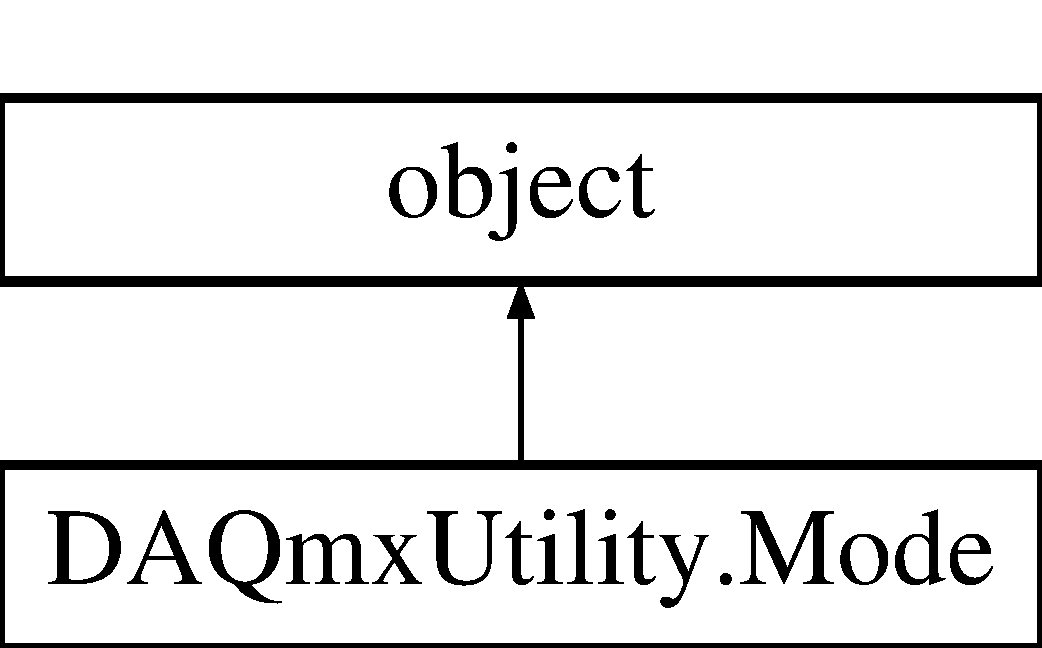
\includegraphics[height=2.000000cm]{class_d_a_qmx_utility_1_1_mode}
\end{center}
\end{figure}
\subsection*{Static Public Attributes}
\begin{DoxyCompactItemize}
\item 
int \hyperlink{class_d_a_qmx_utility_1_1_mode_aedf31db1abedc987384fa876f205b6e3}{Finite} 0
\begin{DoxyCompactList}\small\item\em The Finite mode is a mode where a finite number of samples are generated. \end{DoxyCompactList}\item 
int \hyperlink{class_d_a_qmx_utility_1_1_mode_a9e5a660549cbb0b432aec68a78e95ecd}{Continuous} 1
\begin{DoxyCompactList}\small\item\em The Continuous mode is a mode where a set of samples are continuously repeated. \end{DoxyCompactList}\item 
int \hyperlink{class_d_a_qmx_utility_1_1_mode_aeb3dddf49d2987e35fe408bc53b2e0ec}{Static} 2
\begin{DoxyCompactList}\small\item\em The Static mode is a mode where only one sample is generated. \end{DoxyCompactList}\end{DoxyCompactItemize}


\subsection{Detailed Description}
This class defines the mode variable which is used as an enumerated typedef. 



\subsection{Member Data Documentation}
\hypertarget{class_d_a_qmx_utility_1_1_mode_a9e5a660549cbb0b432aec68a78e95ecd}{\index{D\-A\-Qmx\-Utility\-::\-Mode@{D\-A\-Qmx\-Utility\-::\-Mode}!Continuous@{Continuous}}
\index{Continuous@{Continuous}!DAQmxUtility::Mode@{D\-A\-Qmx\-Utility\-::\-Mode}}
\subsubsection[{Continuous}]{\setlength{\rightskip}{0pt plus 5cm}int D\-A\-Qmx\-Utility.\-Mode.\-Continuous 1\hspace{0.3cm}{\ttfamily [static]}}}\label{class_d_a_qmx_utility_1_1_mode_a9e5a660549cbb0b432aec68a78e95ecd}


The Continuous mode is a mode where a set of samples are continuously repeated. 

They samples are repeared until the stop() method is called. Default value\-: 1. \hypertarget{class_d_a_qmx_utility_1_1_mode_aedf31db1abedc987384fa876f205b6e3}{\index{D\-A\-Qmx\-Utility\-::\-Mode@{D\-A\-Qmx\-Utility\-::\-Mode}!Finite@{Finite}}
\index{Finite@{Finite}!DAQmxUtility::Mode@{D\-A\-Qmx\-Utility\-::\-Mode}}
\subsubsection[{Finite}]{\setlength{\rightskip}{0pt plus 5cm}int D\-A\-Qmx\-Utility.\-Mode.\-Finite 0\hspace{0.3cm}{\ttfamily [static]}}}\label{class_d_a_qmx_utility_1_1_mode_aedf31db1abedc987384fa876f205b6e3}


The Finite mode is a mode where a finite number of samples are generated. 

Default value\-: 0. \hypertarget{class_d_a_qmx_utility_1_1_mode_aeb3dddf49d2987e35fe408bc53b2e0ec}{\index{D\-A\-Qmx\-Utility\-::\-Mode@{D\-A\-Qmx\-Utility\-::\-Mode}!Static@{Static}}
\index{Static@{Static}!DAQmxUtility::Mode@{D\-A\-Qmx\-Utility\-::\-Mode}}
\subsubsection[{Static}]{\setlength{\rightskip}{0pt plus 5cm}int D\-A\-Qmx\-Utility.\-Mode.\-Static 2\hspace{0.3cm}{\ttfamily [static]}}}\label{class_d_a_qmx_utility_1_1_mode_aeb3dddf49d2987e35fe408bc53b2e0ec}


The Static mode is a mode where only one sample is generated. 

Default Value\-: 2. 

The documentation for this class was generated from the following file\-:\begin{DoxyCompactItemize}
\item 
D\-A\-Qmx\-Utility.\-py\end{DoxyCompactItemize}

\hypertarget{classni_sync_error_1_1ni_sync_error}{\section{ni\-Sync\-Error.\-ni\-Sync\-Error Class Reference}
\label{classni_sync_error_1_1ni_sync_error}\index{ni\-Sync\-Error.\-ni\-Sync\-Error@{ni\-Sync\-Error.\-ni\-Sync\-Error}}
}


This is a class to handle errors generated by the ni\-Sync python module.  


Inheritance diagram for ni\-Sync\-Error.\-ni\-Sync\-Error\-:\begin{figure}[H]
\begin{center}
\leavevmode
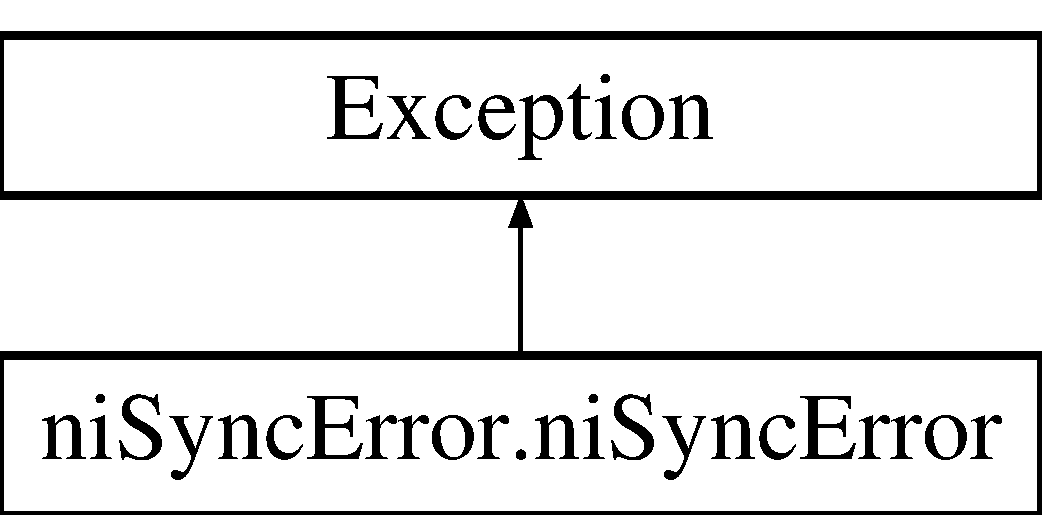
\includegraphics[height=2.000000cm]{classni_sync_error_1_1ni_sync_error}
\end{center}
\end{figure}
\subsection*{Public Member Functions}
\begin{DoxyCompactItemize}
\item 
def \hyperlink{classni_sync_error_1_1ni_sync_error_ac36e2cdbeddc5112ee22e659c15b6fd8}{\-\_\-\-\_\-init\-\_\-\-\_\-}
\begin{DoxyCompactList}\small\item\em This is the constructor of the \hyperlink{classni_sync_error_1_1ni_sync_error}{ni\-Sync\-Error} class. \end{DoxyCompactList}\item 
def \hyperlink{classni_sync_error_1_1ni_sync_error_a1b30d4c0ff582d4f449f1ee140a5c3d0}{\-\_\-\-\_\-str\-\_\-\-\_\-}
\begin{DoxyCompactList}\small\item\em This function returns a string containing the code and message describing the error that occurred. \end{DoxyCompactList}\end{DoxyCompactItemize}
\subsection*{Public Attributes}
\begin{DoxyCompactItemize}
\item 
\hyperlink{classni_sync_error_1_1ni_sync_error_afb0c634f44c362455cb2a9fea5e6c3f5}{code}
\begin{DoxyCompactList}\small\item\em This is the status code returned by the N\-I-\/\-Sync drivers. \end{DoxyCompactList}\item 
\hyperlink{classni_sync_error_1_1ni_sync_error_a39eb7e5776539d5bbacf7815cbfbd180}{msg}
\begin{DoxyCompactList}\small\item\em This is the message returned by the N\-I-\/\-Sync drivers. \end{DoxyCompactList}\end{DoxyCompactItemize}


\subsection{Detailed Description}
This is a class to handle errors generated by the ni\-Sync python module. 



\subsection{Constructor \& Destructor Documentation}
\hypertarget{classni_sync_error_1_1ni_sync_error_ac36e2cdbeddc5112ee22e659c15b6fd8}{\index{ni\-Sync\-Error\-::ni\-Sync\-Error@{ni\-Sync\-Error\-::ni\-Sync\-Error}!\-\_\-\-\_\-init\-\_\-\-\_\-@{\-\_\-\-\_\-init\-\_\-\-\_\-}}
\index{\-\_\-\-\_\-init\-\_\-\-\_\-@{\-\_\-\-\_\-init\-\_\-\-\_\-}!niSyncError::niSyncError@{ni\-Sync\-Error\-::ni\-Sync\-Error}}
\subsubsection[{\-\_\-\-\_\-init\-\_\-\-\_\-}]{\setlength{\rightskip}{0pt plus 5cm}def ni\-Sync\-Error.\-ni\-Sync\-Error.\-\_\-\-\_\-init\-\_\-\-\_\- (
\begin{DoxyParamCaption}
\item[{}]{self, }
\item[{}]{code, }
\item[{}]{msg}
\end{DoxyParamCaption}
)}}\label{classni_sync_error_1_1ni_sync_error_ac36e2cdbeddc5112ee22e659c15b6fd8}


This is the constructor of the \hyperlink{classni_sync_error_1_1ni_sync_error}{ni\-Sync\-Error} class. 



\subsection{Member Function Documentation}
\hypertarget{classni_sync_error_1_1ni_sync_error_a1b30d4c0ff582d4f449f1ee140a5c3d0}{\index{ni\-Sync\-Error\-::ni\-Sync\-Error@{ni\-Sync\-Error\-::ni\-Sync\-Error}!\-\_\-\-\_\-str\-\_\-\-\_\-@{\-\_\-\-\_\-str\-\_\-\-\_\-}}
\index{\-\_\-\-\_\-str\-\_\-\-\_\-@{\-\_\-\-\_\-str\-\_\-\-\_\-}!niSyncError::niSyncError@{ni\-Sync\-Error\-::ni\-Sync\-Error}}
\subsubsection[{\-\_\-\-\_\-str\-\_\-\-\_\-}]{\setlength{\rightskip}{0pt plus 5cm}def ni\-Sync\-Error.\-ni\-Sync\-Error.\-\_\-\-\_\-str\-\_\-\-\_\- (
\begin{DoxyParamCaption}
\item[{}]{self}
\end{DoxyParamCaption}
)}}\label{classni_sync_error_1_1ni_sync_error_a1b30d4c0ff582d4f449f1ee140a5c3d0}


This function returns a string containing the code and message describing the error that occurred. 

This strig will be displayed to the stderr output when a N\-I-\/\-Sync error occurs. 

\subsection{Member Data Documentation}
\hypertarget{classni_sync_error_1_1ni_sync_error_afb0c634f44c362455cb2a9fea5e6c3f5}{\index{ni\-Sync\-Error\-::ni\-Sync\-Error@{ni\-Sync\-Error\-::ni\-Sync\-Error}!code@{code}}
\index{code@{code}!niSyncError::niSyncError@{ni\-Sync\-Error\-::ni\-Sync\-Error}}
\subsubsection[{code}]{\setlength{\rightskip}{0pt plus 5cm}ni\-Sync\-Error.\-ni\-Sync\-Error.\-code}}\label{classni_sync_error_1_1ni_sync_error_afb0c634f44c362455cb2a9fea5e6c3f5}


This is the status code returned by the N\-I-\/\-Sync drivers. 

The code value is useful, because error codes can be searched on the National Instruments website (www.\-ni.\-com). \hypertarget{classni_sync_error_1_1ni_sync_error_a39eb7e5776539d5bbacf7815cbfbd180}{\index{ni\-Sync\-Error\-::ni\-Sync\-Error@{ni\-Sync\-Error\-::ni\-Sync\-Error}!msg@{msg}}
\index{msg@{msg}!niSyncError::niSyncError@{ni\-Sync\-Error\-::ni\-Sync\-Error}}
\subsubsection[{msg}]{\setlength{\rightskip}{0pt plus 5cm}ni\-Sync\-Error.\-ni\-Sync\-Error.\-msg}}\label{classni_sync_error_1_1ni_sync_error_a39eb7e5776539d5bbacf7815cbfbd180}


This is the message returned by the N\-I-\/\-Sync drivers. 

The message give a more detailed explanation as to why an error occurred. 

The documentation for this class was generated from the following file\-:\begin{DoxyCompactItemize}
\item 
ni\-Sync\-Error.\-py\end{DoxyCompactItemize}

\hypertarget{class_timing_1_1_timing}{\section{Timing.\-Timing Class Reference}
\label{class_timing_1_1_timing}\index{Timing.\-Timing@{Timing.\-Timing}}
}


This class will generate perform the timing and synchronization required to synchronize all cards on the P\-X\-I backplane.  


Inheritance diagram for Timing.\-Timing\-:\begin{figure}[H]
\begin{center}
\leavevmode
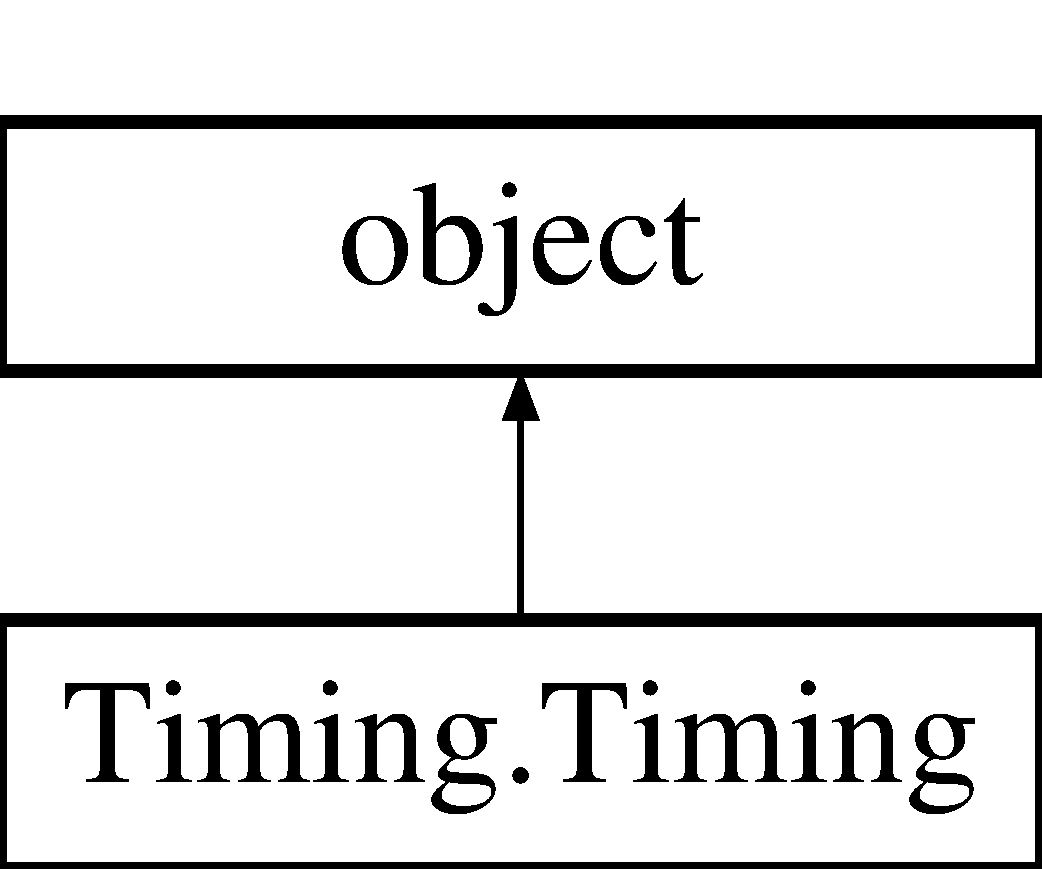
\includegraphics[height=2.000000cm]{class_timing_1_1_timing}
\end{center}
\end{figure}
\subsection*{Public Member Functions}
\begin{DoxyCompactItemize}
\item 
def \hyperlink{class_timing_1_1_timing_ac67aaac1d30dc11a6924a06c099f4fa1}{\-\_\-\-\_\-init\-\_\-\-\_\-}
\begin{DoxyCompactList}\small\item\em This function is a constructor for the \hyperlink{class_timing_1_1_timing}{Timing} class. \end{DoxyCompactList}\item 
def \hyperlink{class_timing_1_1_timing_a74750a56a2403b952fdd78e9d67f6b88}{init}
\begin{DoxyCompactList}\small\item\em This function connects to the ni\-Sync device and starts to setup clock and trigger connections. \end{DoxyCompactList}\item 
def \hyperlink{class_timing_1_1_timing_a464d13b21bd536d8332808cafb946725}{send\-Software\-Trigger}
\begin{DoxyCompactList}\small\item\em This function will send a trigger to all devices when it is called. \end{DoxyCompactList}\item 
def \hyperlink{class_timing_1_1_timing_a1d63d7de0f640dfac6b236a242d75d4d}{close}
\begin{DoxyCompactList}\small\item\em This function will close the connection to the ni\-Sync device. \end{DoxyCompactList}\item 
def \hyperlink{class_timing_1_1_timing_aa351ebd1126df7ce0711f2dd90f054be}{\-\_\-\-\_\-del\-\_\-\-\_\-}
\begin{DoxyCompactList}\small\item\em This is the destructor for the \hyperlink{class_timing_1_1_timing}{Timing} class. \end{DoxyCompactList}\end{DoxyCompactItemize}
\subsection*{Public Attributes}
\begin{DoxyCompactItemize}
\item 
\hyperlink{class_timing_1_1_timing_ac6ffaf6ca94b488dba1c56a780b01cfb}{session}
\begin{DoxyCompactList}\small\item\em This is the reference to the N\-I-\/\-Sync session. \end{DoxyCompactList}\item 
\hyperlink{class_timing_1_1_timing_a8ce8605fb1b55c4a7a0db05c6b1a551c}{resource\-Name}
\begin{DoxyCompactList}\small\item\em This the name of the N\-I-\/\-Sync resource that refers to the synchronization P\-X\-I card. \end{DoxyCompactList}\item 
\hyperlink{class_timing_1_1_timing_aa54e754e141f10df585dbe3bf86729ef}{status}
\begin{DoxyCompactList}\small\item\em This is the status of the N\-I-\/\-Sync session. \end{DoxyCompactList}\item 
\hyperlink{class_timing_1_1_timing_a802c666b56edd255e17036d5317af75c}{initialized}
\begin{DoxyCompactList}\small\item\em This is a boolean that is true when the N\-I-\/\-Sync session has been initialized. \end{DoxyCompactList}\item 
\hyperlink{class_timing_1_1_timing_a645c0a6e372274c15036da2cdd81ce51}{sample\-Rate}
\begin{DoxyCompactList}\small\item\em This is the sample rate of the sample clock that gets distributed to all of the cards on a P\-X\-I Chassis. \end{DoxyCompactList}\item 
\hyperlink{class_timing_1_1_timing_acb98ae4190c94c258c1f86060ab27a86}{divisor}
\begin{DoxyCompactList}\small\item\em The dds is used to generate the sample clock. \end{DoxyCompactList}\item 
\hyperlink{class_timing_1_1_timing_a6df1c9bf5ff79f8f93242f2f52d5c38a}{dds\-Freq}
\begin{DoxyCompactList}\small\item\em This is the D\-D\-S frequency that is calculated from the sample rate and the divisor. \end{DoxyCompactList}\item 
\hyperlink{class_timing_1_1_timing_a42cacaad767cfee65072c72471a5b3a6}{pxi\-Star\-Slots}
\begin{DoxyCompactList}\small\item\em This is the number of pxi star slots available on the chassis. \end{DoxyCompactList}\end{DoxyCompactItemize}


\subsection{Detailed Description}
This class will generate perform the timing and synchronization required to synchronize all cards on the P\-X\-I backplane. 



\subsection{Constructor \& Destructor Documentation}
\hypertarget{class_timing_1_1_timing_ac67aaac1d30dc11a6924a06c099f4fa1}{\index{Timing\-::\-Timing@{Timing\-::\-Timing}!\-\_\-\-\_\-init\-\_\-\-\_\-@{\-\_\-\-\_\-init\-\_\-\-\_\-}}
\index{\-\_\-\-\_\-init\-\_\-\-\_\-@{\-\_\-\-\_\-init\-\_\-\-\_\-}!Timing::Timing@{Timing\-::\-Timing}}
\subsubsection[{\-\_\-\-\_\-init\-\_\-\-\_\-}]{\setlength{\rightskip}{0pt plus 5cm}def Timing.\-Timing.\-\_\-\-\_\-init\-\_\-\-\_\- (
\begin{DoxyParamCaption}
\item[{}]{self}
\end{DoxyParamCaption}
)}}\label{class_timing_1_1_timing_ac67aaac1d30dc11a6924a06c099f4fa1}


This function is a constructor for the \hyperlink{class_timing_1_1_timing}{Timing} class. 


\begin{DoxyParams}{Parameters}
{\em self} & The object pointer. \\
\hline
\end{DoxyParams}
\hypertarget{class_timing_1_1_timing_aa351ebd1126df7ce0711f2dd90f054be}{\index{Timing\-::\-Timing@{Timing\-::\-Timing}!\-\_\-\-\_\-del\-\_\-\-\_\-@{\-\_\-\-\_\-del\-\_\-\-\_\-}}
\index{\-\_\-\-\_\-del\-\_\-\-\_\-@{\-\_\-\-\_\-del\-\_\-\-\_\-}!Timing::Timing@{Timing\-::\-Timing}}
\subsubsection[{\-\_\-\-\_\-del\-\_\-\-\_\-}]{\setlength{\rightskip}{0pt plus 5cm}def Timing.\-Timing.\-\_\-\-\_\-del\-\_\-\-\_\- (
\begin{DoxyParamCaption}
\item[{}]{self}
\end{DoxyParamCaption}
)}}\label{class_timing_1_1_timing_aa351ebd1126df7ce0711f2dd90f054be}


This is the destructor for the \hyperlink{class_timing_1_1_timing}{Timing} class. 


\begin{DoxyParams}{Parameters}
{\em self} & The object pointer. \\
\hline
\end{DoxyParams}


\subsection{Member Function Documentation}
\hypertarget{class_timing_1_1_timing_a1d63d7de0f640dfac6b236a242d75d4d}{\index{Timing\-::\-Timing@{Timing\-::\-Timing}!close@{close}}
\index{close@{close}!Timing::Timing@{Timing\-::\-Timing}}
\subsubsection[{close}]{\setlength{\rightskip}{0pt plus 5cm}def Timing.\-Timing.\-close (
\begin{DoxyParamCaption}
\item[{}]{self}
\end{DoxyParamCaption}
)}}\label{class_timing_1_1_timing_a1d63d7de0f640dfac6b236a242d75d4d}


This function will close the connection to the ni\-Sync device. 


\begin{DoxyParams}{Parameters}
{\em self} & The object pointer. \\
\hline
\end{DoxyParams}
\hypertarget{class_timing_1_1_timing_a74750a56a2403b952fdd78e9d67f6b88}{\index{Timing\-::\-Timing@{Timing\-::\-Timing}!init@{init}}
\index{init@{init}!Timing::Timing@{Timing\-::\-Timing}}
\subsubsection[{init}]{\setlength{\rightskip}{0pt plus 5cm}def Timing.\-Timing.\-init (
\begin{DoxyParamCaption}
\item[{}]{self, }
\item[{}]{device\-Name}
\end{DoxyParamCaption}
)}}\label{class_timing_1_1_timing_a74750a56a2403b952fdd78e9d67f6b88}


This function connects to the ni\-Sync device and starts to setup clock and trigger connections. 


\begin{DoxyParams}{Parameters}
{\em self} & The object pointer. \\
\hline
{\em device\-Name} & The name of the ni\-Sync device. This name can be found in Measurement and Automation Explorer. Example value\-: \char`\"{}\-P\-X\-I1\-Slot14\char`\"{} \\
\hline
\end{DoxyParams}
\hypertarget{class_timing_1_1_timing_a464d13b21bd536d8332808cafb946725}{\index{Timing\-::\-Timing@{Timing\-::\-Timing}!send\-Software\-Trigger@{send\-Software\-Trigger}}
\index{send\-Software\-Trigger@{send\-Software\-Trigger}!Timing::Timing@{Timing\-::\-Timing}}
\subsubsection[{send\-Software\-Trigger}]{\setlength{\rightskip}{0pt plus 5cm}def Timing.\-Timing.\-send\-Software\-Trigger (
\begin{DoxyParamCaption}
\item[{}]{self}
\end{DoxyParamCaption}
)}}\label{class_timing_1_1_timing_a464d13b21bd536d8332808cafb946725}


This function will send a trigger to all devices when it is called. 


\begin{DoxyParams}{Parameters}
{\em self} & The object pointer. \\
\hline
\end{DoxyParams}


\subsection{Member Data Documentation}
\hypertarget{class_timing_1_1_timing_a6df1c9bf5ff79f8f93242f2f52d5c38a}{\index{Timing\-::\-Timing@{Timing\-::\-Timing}!dds\-Freq@{dds\-Freq}}
\index{dds\-Freq@{dds\-Freq}!Timing::Timing@{Timing\-::\-Timing}}
\subsubsection[{dds\-Freq}]{\setlength{\rightskip}{0pt plus 5cm}Timing.\-Timing.\-dds\-Freq}}\label{class_timing_1_1_timing_a6df1c9bf5ff79f8f93242f2f52d5c38a}


This is the D\-D\-S frequency that is calculated from the sample rate and the divisor. 

The D\-D\-S frequency is the sample rate divided by the divisor. \hypertarget{class_timing_1_1_timing_acb98ae4190c94c258c1f86060ab27a86}{\index{Timing\-::\-Timing@{Timing\-::\-Timing}!divisor@{divisor}}
\index{divisor@{divisor}!Timing::Timing@{Timing\-::\-Timing}}
\subsubsection[{divisor}]{\setlength{\rightskip}{0pt plus 5cm}Timing.\-Timing.\-divisor}}\label{class_timing_1_1_timing_acb98ae4190c94c258c1f86060ab27a86}


The dds is used to generate the sample clock. 

The lower the value of the divisor the more inaccurate the sample clock. This value is defualted to its maximum of 32. \hypertarget{class_timing_1_1_timing_a802c666b56edd255e17036d5317af75c}{\index{Timing\-::\-Timing@{Timing\-::\-Timing}!initialized@{initialized}}
\index{initialized@{initialized}!Timing::Timing@{Timing\-::\-Timing}}
\subsubsection[{initialized}]{\setlength{\rightskip}{0pt plus 5cm}Timing.\-Timing.\-initialized}}\label{class_timing_1_1_timing_a802c666b56edd255e17036d5317af75c}


This is a boolean that is true when the N\-I-\/\-Sync session has been initialized. 

\hypertarget{class_timing_1_1_timing_a42cacaad767cfee65072c72471a5b3a6}{\index{Timing\-::\-Timing@{Timing\-::\-Timing}!pxi\-Star\-Slots@{pxi\-Star\-Slots}}
\index{pxi\-Star\-Slots@{pxi\-Star\-Slots}!Timing::Timing@{Timing\-::\-Timing}}
\subsubsection[{pxi\-Star\-Slots}]{\setlength{\rightskip}{0pt plus 5cm}Timing.\-Timing.\-pxi\-Star\-Slots}}\label{class_timing_1_1_timing_a42cacaad767cfee65072c72471a5b3a6}


This is the number of pxi star slots available on the chassis. 

In order for the sample clock to be distributed to all cards, this value must be equal to or larger than the number of potential cards on the Chassis. \hypertarget{class_timing_1_1_timing_a8ce8605fb1b55c4a7a0db05c6b1a551c}{\index{Timing\-::\-Timing@{Timing\-::\-Timing}!resource\-Name@{resource\-Name}}
\index{resource\-Name@{resource\-Name}!Timing::Timing@{Timing\-::\-Timing}}
\subsubsection[{resource\-Name}]{\setlength{\rightskip}{0pt plus 5cm}Timing.\-Timing.\-resource\-Name}}\label{class_timing_1_1_timing_a8ce8605fb1b55c4a7a0db05c6b1a551c}


This the name of the N\-I-\/\-Sync resource that refers to the synchronization P\-X\-I card. 

\hypertarget{class_timing_1_1_timing_a645c0a6e372274c15036da2cdd81ce51}{\index{Timing\-::\-Timing@{Timing\-::\-Timing}!sample\-Rate@{sample\-Rate}}
\index{sample\-Rate@{sample\-Rate}!Timing::Timing@{Timing\-::\-Timing}}
\subsubsection[{sample\-Rate}]{\setlength{\rightskip}{0pt plus 5cm}Timing.\-Timing.\-sample\-Rate}}\label{class_timing_1_1_timing_a645c0a6e372274c15036da2cdd81ce51}


This is the sample rate of the sample clock that gets distributed to all of the cards on a P\-X\-I Chassis. 

\hypertarget{class_timing_1_1_timing_ac6ffaf6ca94b488dba1c56a780b01cfb}{\index{Timing\-::\-Timing@{Timing\-::\-Timing}!session@{session}}
\index{session@{session}!Timing::Timing@{Timing\-::\-Timing}}
\subsubsection[{session}]{\setlength{\rightskip}{0pt plus 5cm}Timing.\-Timing.\-session}}\label{class_timing_1_1_timing_ac6ffaf6ca94b488dba1c56a780b01cfb}


This is the reference to the N\-I-\/\-Sync session. 

\hypertarget{class_timing_1_1_timing_aa54e754e141f10df585dbe3bf86729ef}{\index{Timing\-::\-Timing@{Timing\-::\-Timing}!status@{status}}
\index{status@{status}!Timing::Timing@{Timing\-::\-Timing}}
\subsubsection[{status}]{\setlength{\rightskip}{0pt plus 5cm}Timing.\-Timing.\-status}}\label{class_timing_1_1_timing_aa54e754e141f10df585dbe3bf86729ef}


This is the status of the N\-I-\/\-Sync session. 

A value greater than 0 means that an error has occurred. When the status is greater than 0 an error should be reported by the class. 

The documentation for this class was generated from the following file\-:\begin{DoxyCompactItemize}
\item 
Timing.\-py\end{DoxyCompactItemize}

\hypertarget{class_d_a_qmx_utility_1_1_trigger_type}{\section{D\-A\-Qmx\-Utility.\-Trigger\-Type Class Reference}
\label{class_d_a_qmx_utility_1_1_trigger_type}\index{D\-A\-Qmx\-Utility.\-Trigger\-Type@{D\-A\-Qmx\-Utility.\-Trigger\-Type}}
}


This class defines the trigger type variable which is used as an enumerated typedef.  


Inheritance diagram for D\-A\-Qmx\-Utility.\-Trigger\-Type\-:\begin{figure}[H]
\begin{center}
\leavevmode
\includegraphics[height=2.000000cm]{class_d_a_qmx_utility_1_1_trigger_type}
\end{center}
\end{figure}
\subsection*{Static Public Attributes}
\begin{DoxyCompactItemize}
\item 
int \hyperlink{class_d_a_qmx_utility_1_1_trigger_type_a7427a18d64562c6221627ae8fc80da93}{Software} 0
\begin{DoxyCompactList}\small\item\em The Software trigger type is used when a single software command starts the signal generation. \end{DoxyCompactList}\item 
int \hyperlink{class_d_a_qmx_utility_1_1_trigger_type_a52598eae33e8cc6021f037a0c79e8500}{Hardware} 1
\begin{DoxyCompactList}\small\item\em The Hardware trigger types is used when a start trigger is utilized to start the signal generation. \end{DoxyCompactList}\end{DoxyCompactItemize}


\subsection{Detailed Description}
This class defines the trigger type variable which is used as an enumerated typedef. 



\subsection{Member Data Documentation}
\hypertarget{class_d_a_qmx_utility_1_1_trigger_type_a52598eae33e8cc6021f037a0c79e8500}{\index{D\-A\-Qmx\-Utility\-::\-Trigger\-Type@{D\-A\-Qmx\-Utility\-::\-Trigger\-Type}!Hardware@{Hardware}}
\index{Hardware@{Hardware}!DAQmxUtility::TriggerType@{D\-A\-Qmx\-Utility\-::\-Trigger\-Type}}
\subsubsection[{Hardware}]{\setlength{\rightskip}{0pt plus 5cm}int D\-A\-Qmx\-Utility.\-Trigger\-Type.\-Hardware 1\hspace{0.3cm}{\ttfamily [static]}}}\label{class_d_a_qmx_utility_1_1_trigger_type_a52598eae33e8cc6021f037a0c79e8500}


The Hardware trigger types is used when a start trigger is utilized to start the signal generation. 

A software command may still be used to start the generation. However, that command will set the generator to wait for a trigger such that all signal are synchronized. Defualt value\-: 1 \hypertarget{class_d_a_qmx_utility_1_1_trigger_type_a7427a18d64562c6221627ae8fc80da93}{\index{D\-A\-Qmx\-Utility\-::\-Trigger\-Type@{D\-A\-Qmx\-Utility\-::\-Trigger\-Type}!Software@{Software}}
\index{Software@{Software}!DAQmxUtility::TriggerType@{D\-A\-Qmx\-Utility\-::\-Trigger\-Type}}
\subsubsection[{Software}]{\setlength{\rightskip}{0pt plus 5cm}int D\-A\-Qmx\-Utility.\-Trigger\-Type.\-Software 0\hspace{0.3cm}{\ttfamily [static]}}}\label{class_d_a_qmx_utility_1_1_trigger_type_a7427a18d64562c6221627ae8fc80da93}


The Software trigger type is used when a single software command starts the signal generation. 

Default value\-: 0. 

The documentation for this class was generated from the following file\-:\begin{DoxyCompactItemize}
\item 
D\-A\-Qmx\-Utility.\-py\end{DoxyCompactItemize}

\hypertarget{class_waveform_chassis_1_1_waveform_chassis}{\section{Waveform\-Chassis.\-Waveform\-Chassis Class Reference}
\label{class_waveform_chassis_1_1_waveform_chassis}\index{Waveform\-Chassis.\-Waveform\-Chassis@{Waveform\-Chassis.\-Waveform\-Chassis}}
}


This class contains a list of Waveform\-Generator objects and a Timing object.  


Inheritance diagram for Waveform\-Chassis.\-Waveform\-Chassis\-:\begin{figure}[H]
\begin{center}
\leavevmode
\includegraphics[height=2.000000cm]{class_waveform_chassis_1_1_waveform_chassis}
\end{center}
\end{figure}
\subsection*{Public Member Functions}
\begin{DoxyCompactItemize}
\item 
def \hyperlink{class_waveform_chassis_1_1_waveform_chassis_a5b9740879596dbe1422d47dacfaf5f6a}{\-\_\-\-\_\-init\-\_\-\-\_\-}
\begin{DoxyCompactList}\small\item\em This function is a constructor for the \hyperlink{class_waveform_chassis_1_1_waveform_chassis}{Waveform\-Chassis} class. \end{DoxyCompactList}\item 
def \hyperlink{class_waveform_chassis_1_1_waveform_chassis_acd9ab0cb2573d71efcdbf86fb731a95c}{init}
\begin{DoxyCompactList}\small\item\em Initializes the waveform chassis based on the object's configuration. \end{DoxyCompactList}\item 
def \hyperlink{class_waveform_chassis_1_1_waveform_chassis_a81d7ac137a7779ca0dd6ef8492c6030a}{init\-From\-File}
\begin{DoxyCompactList}\small\item\em This function will initialize the waveform chassis based on the configuration file specified by the file\-Path parameter. \end{DoxyCompactList}\item 
def \hyperlink{class_waveform_chassis_1_1_waveform_chassis_a6fee2bcdaeebeda998be000c1892516e}{get\-Num\-Ao\-Channels}
\begin{DoxyCompactList}\small\item\em This function returns the total number of A\-O channels configured. \end{DoxyCompactList}\item 
def \hyperlink{class_waveform_chassis_1_1_waveform_chassis_aa22034c8b518ce28bdf7bcf9f26925ec}{get\-Num\-Do\-Channels}
\begin{DoxyCompactList}\small\item\em This function returns the total number of A\-O channels configured. \end{DoxyCompactList}\item 
def \hyperlink{class_waveform_chassis_1_1_waveform_chassis_a744d35788b29af622f30aa20bb2510b0}{create\-Ao\-Sine\-Buffer}
\begin{DoxyCompactList}\small\item\em This function returns a 1\-D numpy array of sine waves -\/ one for each channel configured by the init function. \end{DoxyCompactList}\item 
def \hyperlink{class_waveform_chassis_1_1_waveform_chassis_a8c1f18f988b85405c9897d502c57454c}{create\-Do\-Test\-Buffer}
\begin{DoxyCompactList}\small\item\em This function returns a 1d array of random U8s for writing to the buffer of digital output channels. \end{DoxyCompactList}\item 
def \hyperlink{class_waveform_chassis_1_1_waveform_chassis_a42bdd67d68a729ad072aaf83de646dd8}{write\-Ao\-Buffer}
\begin{DoxyCompactList}\small\item\em This function will write data into the buffer of the analog outputs that are a part of the \hyperlink{class_waveform_chassis_1_1_waveform_chassis}{Waveform\-Chassis} class. \end{DoxyCompactList}\item 
def \hyperlink{class_waveform_chassis_1_1_waveform_chassis_a08080ba281bb601f6db05ce47863b81b}{write\-Do\-Buffer}
\begin{DoxyCompactList}\small\item\em This function will write data into the buffer of the digital outputs that are a part of the \hyperlink{class_waveform_chassis_1_1_waveform_chassis}{Waveform\-Chassis}. \end{DoxyCompactList}\item 
def \hyperlink{class_waveform_chassis_1_1_waveform_chassis_a324ff64c0087456811dfea0abeb1a3b6}{start}
\begin{DoxyCompactList}\small\item\em This function starts the analog and digital output generation. \end{DoxyCompactList}\item 
def \hyperlink{class_waveform_chassis_1_1_waveform_chassis_a3b82fba6c96c90d70efc9b3eb031f869}{wait\-Until\-Done}
\begin{DoxyCompactList}\small\item\em This functions waits for the analog and digital output generation to complete. \end{DoxyCompactList}\item 
def \hyperlink{class_waveform_chassis_1_1_waveform_chassis_a96f52784b946d309f98866433d0b2b67}{stop}
\begin{DoxyCompactList}\small\item\em This function stops the analog and digital output generation. \end{DoxyCompactList}\item 
def \hyperlink{class_waveform_chassis_1_1_waveform_chassis_acd992cff6a8139f97bdb8e4c9a083b03}{write\-Start\-Stop}
\begin{DoxyCompactList}\small\item\em This function will perform the write, start, wait\-Until\-Done, and stop functions wrapped in one funciton. \end{DoxyCompactList}\item 
def \hyperlink{class_waveform_chassis_1_1_waveform_chassis_a878b267f7ee8b1146c3f0137f18fda00}{close}
\begin{DoxyCompactList}\small\item\em This function will close connection to the \hyperlink{class_waveform_chassis_1_1_waveform_chassis}{Waveform\-Chassis}. \end{DoxyCompactList}\end{DoxyCompactItemize}
\subsection*{Public Attributes}
\begin{DoxyCompactItemize}
\item 
\hyperlink{class_waveform_chassis_1_1_waveform_chassis_a3893045e5a6a259762feb0ee2f313648}{timing}
\begin{DoxyCompactList}\small\item\em This is a Timing object created using the Timing class. \end{DoxyCompactList}\item 
\hyperlink{class_waveform_chassis_1_1_waveform_chassis_a18dae1f29299d1dbd02b06e0f2b5270c}{use\-Timing}
\begin{DoxyCompactList}\small\item\em This is a boolean value that will be true if the \hyperlink{class_waveform_chassis_1_1_waveform_chassis}{Waveform\-Chassis} is configured to use Timing. \end{DoxyCompactList}\item 
\hyperlink{class_waveform_chassis_1_1_waveform_chassis_a9b7abe44035b7e5077bfe7363221d66f}{gens}
\begin{DoxyCompactList}\small\item\em This is a list of Waveform\-Generator objects created using the Waveform\-Generator class. \end{DoxyCompactList}\item 
\hyperlink{class_waveform_chassis_1_1_waveform_chassis_ab15b973ee2283c67e5178280245fe585}{sample\-Rate}
\begin{DoxyCompactList}\small\item\em This is the sample rate of all the Analog and Digital outputs. \end{DoxyCompactList}\item 
\hyperlink{class_waveform_chassis_1_1_waveform_chassis_aec121d179ad4d3bbc2da3a2469dd2dfa}{samples\-Per\-Channel}
\begin{DoxyCompactList}\small\item\em This is the number of channels configured for the \hyperlink{class_waveform_chassis_1_1_waveform_chassis}{Waveform\-Chassis}. \end{DoxyCompactList}\item 
\hyperlink{class_waveform_chassis_1_1_waveform_chassis_a87be64310be9b7775c6915cbdfa7a2af}{mode}
\begin{DoxyCompactList}\small\item\em This is the mode of operation for all generators. \end{DoxyCompactList}\item 
\hyperlink{class_waveform_chassis_1_1_waveform_chassis_ab1d1e2c6f2742589ae187a6d12c26565}{loops}
\begin{DoxyCompactList}\small\item\em The number of times to iterate over a Finite number of samples. \end{DoxyCompactList}\item 
\hyperlink{class_waveform_chassis_1_1_waveform_chassis_af6dd8a668436712fc2cc9dab2fc8ef6f}{trigger\-Type}
\begin{DoxyCompactList}\small\item\em The trigger type for the analog outputs. \end{DoxyCompactList}\item 
\hyperlink{class_waveform_chassis_1_1_waveform_chassis_a5914d44a4e532bed3845206318dd8407}{clk\-Source}
\begin{DoxyCompactList}\small\item\em This is the sample clock source terminal for every Waveform\-Generator configured in the \hyperlink{class_waveform_chassis_1_1_waveform_chassis}{Waveform\-Chassis}. \end{DoxyCompactList}\item 
\hyperlink{class_waveform_chassis_1_1_waveform_chassis_a73f6eace1feef22a221d458a3809c338}{start\-Trigger\-Source}
\begin{DoxyCompactList}\small\item\em This is the start trigger source terminal for every Waveform\-Generator configured in the \hyperlink{class_waveform_chassis_1_1_waveform_chassis}{Waveform\-Chassis}. \end{DoxyCompactList}\end{DoxyCompactItemize}


\subsection{Detailed Description}
This class contains a list of Waveform\-Generator objects and a Timing object. 

It is intended to represent a chasis with a Ni\-Sync Card and a number of P\-X\-I-\/6733s. 

\subsection{Constructor \& Destructor Documentation}
\hypertarget{class_waveform_chassis_1_1_waveform_chassis_a5b9740879596dbe1422d47dacfaf5f6a}{\index{Waveform\-Chassis\-::\-Waveform\-Chassis@{Waveform\-Chassis\-::\-Waveform\-Chassis}!\-\_\-\-\_\-init\-\_\-\-\_\-@{\-\_\-\-\_\-init\-\_\-\-\_\-}}
\index{\-\_\-\-\_\-init\-\_\-\-\_\-@{\-\_\-\-\_\-init\-\_\-\-\_\-}!WaveformChassis::WaveformChassis@{Waveform\-Chassis\-::\-Waveform\-Chassis}}
\subsubsection[{\-\_\-\-\_\-init\-\_\-\-\_\-}]{\setlength{\rightskip}{0pt plus 5cm}def Waveform\-Chassis.\-Waveform\-Chassis.\-\_\-\-\_\-init\-\_\-\-\_\- (
\begin{DoxyParamCaption}
\item[{}]{self}
\end{DoxyParamCaption}
)}}\label{class_waveform_chassis_1_1_waveform_chassis_a5b9740879596dbe1422d47dacfaf5f6a}


This function is a constructor for the \hyperlink{class_waveform_chassis_1_1_waveform_chassis}{Waveform\-Chassis} class. 

It creates the internal variables required to perform functions within the class. This function does not initialize any hardware. 

\subsection{Member Function Documentation}
\hypertarget{class_waveform_chassis_1_1_waveform_chassis_a878b267f7ee8b1146c3f0137f18fda00}{\index{Waveform\-Chassis\-::\-Waveform\-Chassis@{Waveform\-Chassis\-::\-Waveform\-Chassis}!close@{close}}
\index{close@{close}!WaveformChassis::WaveformChassis@{Waveform\-Chassis\-::\-Waveform\-Chassis}}
\subsubsection[{close}]{\setlength{\rightskip}{0pt plus 5cm}def Waveform\-Chassis.\-Waveform\-Chassis.\-close (
\begin{DoxyParamCaption}
\item[{}]{self}
\end{DoxyParamCaption}
)}}\label{class_waveform_chassis_1_1_waveform_chassis_a878b267f7ee8b1146c3f0137f18fda00}


This function will close connection to the \hyperlink{class_waveform_chassis_1_1_waveform_chassis}{Waveform\-Chassis}. 


\begin{DoxyParams}{Parameters}
{\em self} & The object pointer. \\
\hline
\end{DoxyParams}
\hypertarget{class_waveform_chassis_1_1_waveform_chassis_a744d35788b29af622f30aa20bb2510b0}{\index{Waveform\-Chassis\-::\-Waveform\-Chassis@{Waveform\-Chassis\-::\-Waveform\-Chassis}!create\-Ao\-Sine\-Buffer@{create\-Ao\-Sine\-Buffer}}
\index{create\-Ao\-Sine\-Buffer@{create\-Ao\-Sine\-Buffer}!WaveformChassis::WaveformChassis@{Waveform\-Chassis\-::\-Waveform\-Chassis}}
\subsubsection[{create\-Ao\-Sine\-Buffer}]{\setlength{\rightskip}{0pt plus 5cm}def Waveform\-Chassis.\-Waveform\-Chassis.\-create\-Ao\-Sine\-Buffer (
\begin{DoxyParamCaption}
\item[{}]{self}
\end{DoxyParamCaption}
)}}\label{class_waveform_chassis_1_1_waveform_chassis_a744d35788b29af622f30aa20bb2510b0}


This function returns a 1\-D numpy array of sine waves -\/ one for each channel configured by the init function. 


\begin{DoxyParams}{Parameters}
{\em self} & The object pointer. \\
\hline
\end{DoxyParams}
\hypertarget{class_waveform_chassis_1_1_waveform_chassis_a8c1f18f988b85405c9897d502c57454c}{\index{Waveform\-Chassis\-::\-Waveform\-Chassis@{Waveform\-Chassis\-::\-Waveform\-Chassis}!create\-Do\-Test\-Buffer@{create\-Do\-Test\-Buffer}}
\index{create\-Do\-Test\-Buffer@{create\-Do\-Test\-Buffer}!WaveformChassis::WaveformChassis@{Waveform\-Chassis\-::\-Waveform\-Chassis}}
\subsubsection[{create\-Do\-Test\-Buffer}]{\setlength{\rightskip}{0pt plus 5cm}def Waveform\-Chassis.\-Waveform\-Chassis.\-create\-Do\-Test\-Buffer (
\begin{DoxyParamCaption}
\item[{}]{self}
\end{DoxyParamCaption}
)}}\label{class_waveform_chassis_1_1_waveform_chassis_a8c1f18f988b85405c9897d502c57454c}


This function returns a 1d array of random U8s for writing to the buffer of digital output channels. 


\begin{DoxyParams}{Parameters}
{\em self} & The object pointer. \\
\hline
\end{DoxyParams}
\hypertarget{class_waveform_chassis_1_1_waveform_chassis_a6fee2bcdaeebeda998be000c1892516e}{\index{Waveform\-Chassis\-::\-Waveform\-Chassis@{Waveform\-Chassis\-::\-Waveform\-Chassis}!get\-Num\-Ao\-Channels@{get\-Num\-Ao\-Channels}}
\index{get\-Num\-Ao\-Channels@{get\-Num\-Ao\-Channels}!WaveformChassis::WaveformChassis@{Waveform\-Chassis\-::\-Waveform\-Chassis}}
\subsubsection[{get\-Num\-Ao\-Channels}]{\setlength{\rightskip}{0pt plus 5cm}def Waveform\-Chassis.\-Waveform\-Chassis.\-get\-Num\-Ao\-Channels (
\begin{DoxyParamCaption}
\item[{}]{self}
\end{DoxyParamCaption}
)}}\label{class_waveform_chassis_1_1_waveform_chassis_a6fee2bcdaeebeda998be000c1892516e}


This function returns the total number of A\-O channels configured. 


\begin{DoxyParams}{Parameters}
{\em self} & The object pointer. \\
\hline
\end{DoxyParams}
\hypertarget{class_waveform_chassis_1_1_waveform_chassis_aa22034c8b518ce28bdf7bcf9f26925ec}{\index{Waveform\-Chassis\-::\-Waveform\-Chassis@{Waveform\-Chassis\-::\-Waveform\-Chassis}!get\-Num\-Do\-Channels@{get\-Num\-Do\-Channels}}
\index{get\-Num\-Do\-Channels@{get\-Num\-Do\-Channels}!WaveformChassis::WaveformChassis@{Waveform\-Chassis\-::\-Waveform\-Chassis}}
\subsubsection[{get\-Num\-Do\-Channels}]{\setlength{\rightskip}{0pt plus 5cm}def Waveform\-Chassis.\-Waveform\-Chassis.\-get\-Num\-Do\-Channels (
\begin{DoxyParamCaption}
\item[{}]{self}
\end{DoxyParamCaption}
)}}\label{class_waveform_chassis_1_1_waveform_chassis_aa22034c8b518ce28bdf7bcf9f26925ec}


This function returns the total number of A\-O channels configured. 


\begin{DoxyParams}{Parameters}
{\em self} & The object pointer. \\
\hline
\end{DoxyParams}
\hypertarget{class_waveform_chassis_1_1_waveform_chassis_acd9ab0cb2573d71efcdbf86fb731a95c}{\index{Waveform\-Chassis\-::\-Waveform\-Chassis@{Waveform\-Chassis\-::\-Waveform\-Chassis}!init@{init}}
\index{init@{init}!WaveformChassis::WaveformChassis@{Waveform\-Chassis\-::\-Waveform\-Chassis}}
\subsubsection[{init}]{\setlength{\rightskip}{0pt plus 5cm}def Waveform\-Chassis.\-Waveform\-Chassis.\-init (
\begin{DoxyParamCaption}
\item[{}]{self, }
\item[{}]{ao\-Devs\-And\-Chnls, }
\item[{}]{do\-Devs\-And\-Chnls = {\ttfamily None}, }
\item[{}]{sync\-Device = {\ttfamily None}}
\end{DoxyParamCaption}
)}}\label{class_waveform_chassis_1_1_waveform_chassis_acd9ab0cb2573d71efcdbf86fb731a95c}


Initializes the waveform chassis based on the object's configuration. 


\begin{DoxyParams}{Parameters}
{\em self} & The object pointer. \\
\hline
{\em ao\-Devs\-And\-Chnls} & This is a list of strings representing the devices and analog output channels. \\
\hline
{\em do\-Devs\-And\-Chnls} & This is a list of strings representing the divices and digital output channels. \\
\hline
{\em sync\-Device} & This is the device name for the N\-I Sync card. \\
\hline
\end{DoxyParams}
\hypertarget{class_waveform_chassis_1_1_waveform_chassis_a81d7ac137a7779ca0dd6ef8492c6030a}{\index{Waveform\-Chassis\-::\-Waveform\-Chassis@{Waveform\-Chassis\-::\-Waveform\-Chassis}!init\-From\-File@{init\-From\-File}}
\index{init\-From\-File@{init\-From\-File}!WaveformChassis::WaveformChassis@{Waveform\-Chassis\-::\-Waveform\-Chassis}}
\subsubsection[{init\-From\-File}]{\setlength{\rightskip}{0pt plus 5cm}def Waveform\-Chassis.\-Waveform\-Chassis.\-init\-From\-File (
\begin{DoxyParamCaption}
\item[{}]{self, }
\item[{}]{file\-Path}
\end{DoxyParamCaption}
)}}\label{class_waveform_chassis_1_1_waveform_chassis_a81d7ac137a7779ca0dd6ef8492c6030a}


This function will initialize the waveform chassis based on the configuration file specified by the file\-Path parameter. 


\begin{DoxyParams}{Parameters}
{\em self} & The object pointer \\
\hline
{\em file\-Path} & The file path to the configuration file. \\
\hline
\end{DoxyParams}
\hypertarget{class_waveform_chassis_1_1_waveform_chassis_a324ff64c0087456811dfea0abeb1a3b6}{\index{Waveform\-Chassis\-::\-Waveform\-Chassis@{Waveform\-Chassis\-::\-Waveform\-Chassis}!start@{start}}
\index{start@{start}!WaveformChassis::WaveformChassis@{Waveform\-Chassis\-::\-Waveform\-Chassis}}
\subsubsection[{start}]{\setlength{\rightskip}{0pt plus 5cm}def Waveform\-Chassis.\-Waveform\-Chassis.\-start (
\begin{DoxyParamCaption}
\item[{}]{self}
\end{DoxyParamCaption}
)}}\label{class_waveform_chassis_1_1_waveform_chassis_a324ff64c0087456811dfea0abeb1a3b6}


This function starts the analog and digital output generation. 


\begin{DoxyParams}{Parameters}
{\em self} & The object pointer. \\
\hline
\end{DoxyParams}
\hypertarget{class_waveform_chassis_1_1_waveform_chassis_a96f52784b946d309f98866433d0b2b67}{\index{Waveform\-Chassis\-::\-Waveform\-Chassis@{Waveform\-Chassis\-::\-Waveform\-Chassis}!stop@{stop}}
\index{stop@{stop}!WaveformChassis::WaveformChassis@{Waveform\-Chassis\-::\-Waveform\-Chassis}}
\subsubsection[{stop}]{\setlength{\rightskip}{0pt plus 5cm}def Waveform\-Chassis.\-Waveform\-Chassis.\-stop (
\begin{DoxyParamCaption}
\item[{}]{self}
\end{DoxyParamCaption}
)}}\label{class_waveform_chassis_1_1_waveform_chassis_a96f52784b946d309f98866433d0b2b67}


This function stops the analog and digital output generation. 


\begin{DoxyParams}{Parameters}
{\em self} & The object pointer. \\
\hline
\end{DoxyParams}
\hypertarget{class_waveform_chassis_1_1_waveform_chassis_a3b82fba6c96c90d70efc9b3eb031f869}{\index{Waveform\-Chassis\-::\-Waveform\-Chassis@{Waveform\-Chassis\-::\-Waveform\-Chassis}!wait\-Until\-Done@{wait\-Until\-Done}}
\index{wait\-Until\-Done@{wait\-Until\-Done}!WaveformChassis::WaveformChassis@{Waveform\-Chassis\-::\-Waveform\-Chassis}}
\subsubsection[{wait\-Until\-Done}]{\setlength{\rightskip}{0pt plus 5cm}def Waveform\-Chassis.\-Waveform\-Chassis.\-wait\-Until\-Done (
\begin{DoxyParamCaption}
\item[{}]{self}
\end{DoxyParamCaption}
)}}\label{class_waveform_chassis_1_1_waveform_chassis_a3b82fba6c96c90d70efc9b3eb031f869}


This functions waits for the analog and digital output generation to complete. 


\begin{DoxyParams}{Parameters}
{\em self} & The object pointer. \\
\hline
\end{DoxyParams}
\hypertarget{class_waveform_chassis_1_1_waveform_chassis_a42bdd67d68a729ad072aaf83de646dd8}{\index{Waveform\-Chassis\-::\-Waveform\-Chassis@{Waveform\-Chassis\-::\-Waveform\-Chassis}!write\-Ao\-Buffer@{write\-Ao\-Buffer}}
\index{write\-Ao\-Buffer@{write\-Ao\-Buffer}!WaveformChassis::WaveformChassis@{Waveform\-Chassis\-::\-Waveform\-Chassis}}
\subsubsection[{write\-Ao\-Buffer}]{\setlength{\rightskip}{0pt plus 5cm}def Waveform\-Chassis.\-Waveform\-Chassis.\-write\-Ao\-Buffer (
\begin{DoxyParamCaption}
\item[{}]{self, }
\item[{}]{data}
\end{DoxyParamCaption}
)}}\label{class_waveform_chassis_1_1_waveform_chassis_a42bdd67d68a729ad072aaf83de646dd8}


This function will write data into the buffer of the analog outputs that are a part of the \hyperlink{class_waveform_chassis_1_1_waveform_chassis}{Waveform\-Chassis} class. 


\begin{DoxyParams}{Parameters}
{\em self} & The object pointer \\
\hline
{\em data} & This is a 1\-D 8-\/bit unsigned integer array that contians data for each digital channel. Channels are non-\/interleaved (channel1 n-\/samples then channel2 n-\/samples). \\
\hline
\end{DoxyParams}
\hypertarget{class_waveform_chassis_1_1_waveform_chassis_a08080ba281bb601f6db05ce47863b81b}{\index{Waveform\-Chassis\-::\-Waveform\-Chassis@{Waveform\-Chassis\-::\-Waveform\-Chassis}!write\-Do\-Buffer@{write\-Do\-Buffer}}
\index{write\-Do\-Buffer@{write\-Do\-Buffer}!WaveformChassis::WaveformChassis@{Waveform\-Chassis\-::\-Waveform\-Chassis}}
\subsubsection[{write\-Do\-Buffer}]{\setlength{\rightskip}{0pt plus 5cm}def Waveform\-Chassis.\-Waveform\-Chassis.\-write\-Do\-Buffer (
\begin{DoxyParamCaption}
\item[{}]{self, }
\item[{}]{data}
\end{DoxyParamCaption}
)}}\label{class_waveform_chassis_1_1_waveform_chassis_a08080ba281bb601f6db05ce47863b81b}


This function will write data into the buffer of the digital outputs that are a part of the \hyperlink{class_waveform_chassis_1_1_waveform_chassis}{Waveform\-Chassis}. 


\begin{DoxyParams}{Parameters}
{\em self} & The object pointer. \\
\hline
{\em data} & This is a 1\-D 8-\/bit unsigned integer array that contians data for each digital channel. Channels are non-\/interleaved (channel1 n-\/samples then channel2 n-\/samples). \\
\hline
\end{DoxyParams}
\hypertarget{class_waveform_chassis_1_1_waveform_chassis_acd992cff6a8139f97bdb8e4c9a083b03}{\index{Waveform\-Chassis\-::\-Waveform\-Chassis@{Waveform\-Chassis\-::\-Waveform\-Chassis}!write\-Start\-Stop@{write\-Start\-Stop}}
\index{write\-Start\-Stop@{write\-Start\-Stop}!WaveformChassis::WaveformChassis@{Waveform\-Chassis\-::\-Waveform\-Chassis}}
\subsubsection[{write\-Start\-Stop}]{\setlength{\rightskip}{0pt plus 5cm}def Waveform\-Chassis.\-Waveform\-Chassis.\-write\-Start\-Stop (
\begin{DoxyParamCaption}
\item[{}]{self, }
\item[{}]{ao\-Data, }
\item[{}]{do\-Data = {\ttfamily None}}
\end{DoxyParamCaption}
)}}\label{class_waveform_chassis_1_1_waveform_chassis_acd992cff6a8139f97bdb8e4c9a083b03}


This function will perform the write, start, wait\-Until\-Done, and stop functions wrapped in one funciton. 

This funciton is no complete and may not exist in a later release!!! 
\begin{DoxyParams}{Parameters}
{\em self} & The object pointer. \\
\hline
\end{DoxyParams}


\subsection{Member Data Documentation}
\hypertarget{class_waveform_chassis_1_1_waveform_chassis_a5914d44a4e532bed3845206318dd8407}{\index{Waveform\-Chassis\-::\-Waveform\-Chassis@{Waveform\-Chassis\-::\-Waveform\-Chassis}!clk\-Source@{clk\-Source}}
\index{clk\-Source@{clk\-Source}!WaveformChassis::WaveformChassis@{Waveform\-Chassis\-::\-Waveform\-Chassis}}
\subsubsection[{clk\-Source}]{\setlength{\rightskip}{0pt plus 5cm}Waveform\-Chassis.\-Waveform\-Chassis.\-clk\-Source}}\label{class_waveform_chassis_1_1_waveform_chassis_a5914d44a4e532bed3845206318dd8407}


This is the sample clock source terminal for every Waveform\-Generator configured in the \hyperlink{class_waveform_chassis_1_1_waveform_chassis}{Waveform\-Chassis}. 

It is defaulted to \char`\"{}\-P\-X\-I\-\_\-\-Star.\char`\"{} \hypertarget{class_waveform_chassis_1_1_waveform_chassis_a9b7abe44035b7e5077bfe7363221d66f}{\index{Waveform\-Chassis\-::\-Waveform\-Chassis@{Waveform\-Chassis\-::\-Waveform\-Chassis}!gens@{gens}}
\index{gens@{gens}!WaveformChassis::WaveformChassis@{Waveform\-Chassis\-::\-Waveform\-Chassis}}
\subsubsection[{gens}]{\setlength{\rightskip}{0pt plus 5cm}Waveform\-Chassis.\-Waveform\-Chassis.\-gens}}\label{class_waveform_chassis_1_1_waveform_chassis_a9b7abe44035b7e5077bfe7363221d66f}


This is a list of Waveform\-Generator objects created using the Waveform\-Generator class. 

It is a list of P\-X\-I6733 cards configured for the \hyperlink{class_waveform_chassis_1_1_waveform_chassis}{Waveform\-Chassis}. \hypertarget{class_waveform_chassis_1_1_waveform_chassis_ab1d1e2c6f2742589ae187a6d12c26565}{\index{Waveform\-Chassis\-::\-Waveform\-Chassis@{Waveform\-Chassis\-::\-Waveform\-Chassis}!loops@{loops}}
\index{loops@{loops}!WaveformChassis::WaveformChassis@{Waveform\-Chassis\-::\-Waveform\-Chassis}}
\subsubsection[{loops}]{\setlength{\rightskip}{0pt plus 5cm}Waveform\-Chassis.\-Waveform\-Chassis.\-loops}}\label{class_waveform_chassis_1_1_waveform_chassis_ab1d1e2c6f2742589ae187a6d12c26565}


The number of times to iterate over a Finite number of samples. 

This value is only useful in the \char`\"{}\-Finite\char`\"{} mode. It is the number of times that a sequence of voltages will be looped. The default is allways 1. \hypertarget{class_waveform_chassis_1_1_waveform_chassis_a87be64310be9b7775c6915cbdfa7a2af}{\index{Waveform\-Chassis\-::\-Waveform\-Chassis@{Waveform\-Chassis\-::\-Waveform\-Chassis}!mode@{mode}}
\index{mode@{mode}!WaveformChassis::WaveformChassis@{Waveform\-Chassis\-::\-Waveform\-Chassis}}
\subsubsection[{mode}]{\setlength{\rightskip}{0pt plus 5cm}Waveform\-Chassis.\-Waveform\-Chassis.\-mode}}\label{class_waveform_chassis_1_1_waveform_chassis_a87be64310be9b7775c6915cbdfa7a2af}


This is the mode of operation for all generators. 

There are currently three modes available. Static mode is where one static voltage is set with no need for a sample clock. Finite mode is where a finite number of voltages will be set at a sample clock rate. Continuous mode is where a sequence of voltages are generated at a sample rate and then repeated until the \hyperlink{class_waveform_chassis_1_1_waveform_chassis_a96f52784b946d309f98866433d0b2b67}{stop()} method is called. \hypertarget{class_waveform_chassis_1_1_waveform_chassis_ab15b973ee2283c67e5178280245fe585}{\index{Waveform\-Chassis\-::\-Waveform\-Chassis@{Waveform\-Chassis\-::\-Waveform\-Chassis}!sample\-Rate@{sample\-Rate}}
\index{sample\-Rate@{sample\-Rate}!WaveformChassis::WaveformChassis@{Waveform\-Chassis\-::\-Waveform\-Chassis}}
\subsubsection[{sample\-Rate}]{\setlength{\rightskip}{0pt plus 5cm}Waveform\-Chassis.\-Waveform\-Chassis.\-sample\-Rate}}\label{class_waveform_chassis_1_1_waveform_chassis_ab15b973ee2283c67e5178280245fe585}


This is the sample rate of all the Analog and Digital outputs. 

The sample rate must be the same for all devices configured in the \hyperlink{class_waveform_chassis_1_1_waveform_chassis}{Waveform\-Chassis}. \hypertarget{class_waveform_chassis_1_1_waveform_chassis_aec121d179ad4d3bbc2da3a2469dd2dfa}{\index{Waveform\-Chassis\-::\-Waveform\-Chassis@{Waveform\-Chassis\-::\-Waveform\-Chassis}!samples\-Per\-Channel@{samples\-Per\-Channel}}
\index{samples\-Per\-Channel@{samples\-Per\-Channel}!WaveformChassis::WaveformChassis@{Waveform\-Chassis\-::\-Waveform\-Chassis}}
\subsubsection[{samples\-Per\-Channel}]{\setlength{\rightskip}{0pt plus 5cm}Waveform\-Chassis.\-Waveform\-Chassis.\-samples\-Per\-Channel}}\label{class_waveform_chassis_1_1_waveform_chassis_aec121d179ad4d3bbc2da3a2469dd2dfa}


This is the number of channels configured for the \hyperlink{class_waveform_chassis_1_1_waveform_chassis}{Waveform\-Chassis}. 

The samples per channel must be the same for all devices configured in the \hyperlink{class_waveform_chassis_1_1_waveform_chassis}{Waveform\-Chassis}. \hypertarget{class_waveform_chassis_1_1_waveform_chassis_a73f6eace1feef22a221d458a3809c338}{\index{Waveform\-Chassis\-::\-Waveform\-Chassis@{Waveform\-Chassis\-::\-Waveform\-Chassis}!start\-Trigger\-Source@{start\-Trigger\-Source}}
\index{start\-Trigger\-Source@{start\-Trigger\-Source}!WaveformChassis::WaveformChassis@{Waveform\-Chassis\-::\-Waveform\-Chassis}}
\subsubsection[{start\-Trigger\-Source}]{\setlength{\rightskip}{0pt plus 5cm}Waveform\-Chassis.\-Waveform\-Chassis.\-start\-Trigger\-Source}}\label{class_waveform_chassis_1_1_waveform_chassis_a73f6eace1feef22a221d458a3809c338}


This is the start trigger source terminal for every Waveform\-Generator configured in the \hyperlink{class_waveform_chassis_1_1_waveform_chassis}{Waveform\-Chassis}. 

It is defaulted to \char`\"{}\-P\-X\-I\-\_\-\-Trig1\char`\"{} \hypertarget{class_waveform_chassis_1_1_waveform_chassis_a3893045e5a6a259762feb0ee2f313648}{\index{Waveform\-Chassis\-::\-Waveform\-Chassis@{Waveform\-Chassis\-::\-Waveform\-Chassis}!timing@{timing}}
\index{timing@{timing}!WaveformChassis::WaveformChassis@{Waveform\-Chassis\-::\-Waveform\-Chassis}}
\subsubsection[{timing}]{\setlength{\rightskip}{0pt plus 5cm}Waveform\-Chassis.\-Waveform\-Chassis.\-timing}}\label{class_waveform_chassis_1_1_waveform_chassis_a3893045e5a6a259762feb0ee2f313648}


This is a Timing object created using the Timing class. 

It is used to synchronize all of the P\-X\-I cards. \hypertarget{class_waveform_chassis_1_1_waveform_chassis_af6dd8a668436712fc2cc9dab2fc8ef6f}{\index{Waveform\-Chassis\-::\-Waveform\-Chassis@{Waveform\-Chassis\-::\-Waveform\-Chassis}!trigger\-Type@{trigger\-Type}}
\index{trigger\-Type@{trigger\-Type}!WaveformChassis::WaveformChassis@{Waveform\-Chassis\-::\-Waveform\-Chassis}}
\subsubsection[{trigger\-Type}]{\setlength{\rightskip}{0pt plus 5cm}Waveform\-Chassis.\-Waveform\-Chassis.\-trigger\-Type}}\label{class_waveform_chassis_1_1_waveform_chassis_af6dd8a668436712fc2cc9dab2fc8ef6f}


The trigger type for the analog outputs. 

There are currently two trigger types -\/ \char`\"{}\-Software\char`\"{} and \char`\"{}\-Hardware.\char`\"{} The \char`\"{}\-Software\char`\"{} mode means that analog output channels are not syncronized. While \char`\"{}\-Hardware\char`\"{} means that analog output channels are syncronized to a start trigger. The start\-Trigger\-Souce attribute must be configured appropriately. \hypertarget{class_waveform_chassis_1_1_waveform_chassis_a18dae1f29299d1dbd02b06e0f2b5270c}{\index{Waveform\-Chassis\-::\-Waveform\-Chassis@{Waveform\-Chassis\-::\-Waveform\-Chassis}!use\-Timing@{use\-Timing}}
\index{use\-Timing@{use\-Timing}!WaveformChassis::WaveformChassis@{Waveform\-Chassis\-::\-Waveform\-Chassis}}
\subsubsection[{use\-Timing}]{\setlength{\rightskip}{0pt plus 5cm}Waveform\-Chassis.\-Waveform\-Chassis.\-use\-Timing}}\label{class_waveform_chassis_1_1_waveform_chassis_a18dae1f29299d1dbd02b06e0f2b5270c}


This is a boolean value that will be true if the \hyperlink{class_waveform_chassis_1_1_waveform_chassis}{Waveform\-Chassis} is configured to use Timing. 



The documentation for this class was generated from the following file\-:\begin{DoxyCompactItemize}
\item 
Waveform\-Chassis.\-py\end{DoxyCompactItemize}

\hypertarget{class_waveform_generator_1_1_waveform_generator}{\section{Waveform\-Generator.\-Waveform\-Generator Class Reference}
\label{class_waveform_generator_1_1_waveform_generator}\index{Waveform\-Generator.\-Waveform\-Generator@{Waveform\-Generator.\-Waveform\-Generator}}
}


This class contains an Analog\-Output and Digital\-Output object.  


Inheritance diagram for Waveform\-Generator.\-Waveform\-Generator\-:\begin{figure}[H]
\begin{center}
\leavevmode
\includegraphics[height=2.000000cm]{class_waveform_generator_1_1_waveform_generator}
\end{center}
\end{figure}
\subsection*{Public Member Functions}
\begin{DoxyCompactItemize}
\item 
def \hyperlink{class_waveform_generator_1_1_waveform_generator_ac7bfc889aae76cae59cfa7de873c3d61}{\-\_\-\-\_\-init\-\_\-\-\_\-}
\begin{DoxyCompactList}\small\item\em This function is a constructor for the \hyperlink{class_waveform_generator_1_1_waveform_generator}{Waveform\-Generator} class. \end{DoxyCompactList}\item 
def \hyperlink{class_waveform_generator_1_1_waveform_generator_a089791e1214bb1342396bef13fcc8a03}{init}
\begin{DoxyCompactList}\small\item\em Initialize the analog and digital outputs based on the object's configuration. \end{DoxyCompactList}\item 
def \hyperlink{class_waveform_generator_1_1_waveform_generator_a9fb983f2822da6a010133da8cf2995f9}{write\-Ao\-Buffer}
\begin{DoxyCompactList}\small\item\em This function writes the specified values into the buffer. \end{DoxyCompactList}\item 
def \hyperlink{class_waveform_generator_1_1_waveform_generator_afeb3e4ca2b30fc3fc4e6e7325ffd9d9f}{write\-Do\-Buffer}
\begin{DoxyCompactList}\small\item\em This function writes the specified values into the buffer. \end{DoxyCompactList}\item 
def \hyperlink{class_waveform_generator_1_1_waveform_generator_a9f7e4db3cb5550802a268ce6a8cb2fb5}{start}
\begin{DoxyCompactList}\small\item\em This function starts the analog and digital output generation. \end{DoxyCompactList}\item 
def \hyperlink{class_waveform_generator_1_1_waveform_generator_ac3cf6e28382592a1f05be72f96d9785f}{wait\-Until\-Done}
\begin{DoxyCompactList}\small\item\em This functions waits for the analog and digital output generation to complete. \end{DoxyCompactList}\item 
def \hyperlink{class_waveform_generator_1_1_waveform_generator_a4e22f830e0cded02a876561c6397de0d}{stop}
\begin{DoxyCompactList}\small\item\em This function stops the analog and digital output generation. \end{DoxyCompactList}\item 
\hypertarget{class_waveform_generator_1_1_waveform_generator_a30ee8b98f7a31f4ed0c28afd72d89930}{def {\bfseries write\-Start\-Stop}}\label{class_waveform_generator_1_1_waveform_generator_a30ee8b98f7a31f4ed0c28afd72d89930}

\item 
def \hyperlink{class_waveform_generator_1_1_waveform_generator_a7bd571409abe468987f15349dc0fa681}{close}
\begin{DoxyCompactList}\small\item\em This function will close connection to the analog and digital ouput device and channels. \end{DoxyCompactList}\end{DoxyCompactItemize}
\subsection*{Public Attributes}
\begin{DoxyCompactItemize}
\item 
\hyperlink{class_waveform_generator_1_1_waveform_generator_ae7ee12ae23b6cf317da47e2580ea1655}{ao}
\begin{DoxyCompactList}\small\item\em This is an Analog\-Output object created using the Analog\-Output class. \end{DoxyCompactList}\item 
\hyperlink{class_waveform_generator_1_1_waveform_generator_a923e4c005cdf1bc1cfdb1cbe33803f40}{do}
\begin{DoxyCompactList}\small\item\em This is a Digital\-Output object created using the Digita\-Output class. \end{DoxyCompactList}\item 
\hyperlink{class_waveform_generator_1_1_waveform_generator_a7f6803ac26eaa8fd4e1880a39c15ca5f}{sample\-Rate}
\begin{DoxyCompactList}\small\item\em This is the sample rate of the waveform generator. \end{DoxyCompactList}\item 
\hyperlink{class_waveform_generator_1_1_waveform_generator_a1800e5e372c200f5241f0ee132b10be3}{samples\-Per\-Channel}
\begin{DoxyCompactList}\small\item\em This is the number of channels configured in the waveform generator. \end{DoxyCompactList}\item 
\hyperlink{class_waveform_generator_1_1_waveform_generator_ae0573744cbc723202afa75c6381e3f71}{clk\-Source}
\begin{DoxyCompactList}\small\item\em This is the sample clock source terminal. \end{DoxyCompactList}\item 
\hyperlink{class_waveform_generator_1_1_waveform_generator_a2eb2105f7a99c224ea725a5fff4c4b39}{start\-Trigger\-Source}
\begin{DoxyCompactList}\small\item\em This is the start trigger source terminal. \end{DoxyCompactList}\item 
\hyperlink{class_waveform_generator_1_1_waveform_generator_ab11b448ff5baf7c87021af3cddfa49d0}{mode}
\begin{DoxyCompactList}\small\item\em There are currently three modes available. \end{DoxyCompactList}\item 
\hyperlink{class_waveform_generator_1_1_waveform_generator_aa36d19f0d2c8700947394d01b6b4621a}{loops}
\begin{DoxyCompactList}\small\item\em This value is only useful in the \char`\"{}\-Finite\char`\"{} mode. \end{DoxyCompactList}\item 
\hyperlink{class_waveform_generator_1_1_waveform_generator_a240878363858425aa6c8d25241479dbf}{trigger\-Type}
\begin{DoxyCompactList}\small\item\em There are currently two trigger types -\/ \char`\"{}\-Software\char`\"{} and \char`\"{}\-Hardware.\char`\"{} The \char`\"{}\-Software\char`\"{} mode means that analog output channels are not syncronized. \end{DoxyCompactList}\item 
\hyperlink{class_waveform_generator_1_1_waveform_generator_abd9a10ccc783ec4174a7ee9f8ab170ad}{use\-Ao}
\begin{DoxyCompactList}\small\item\em This is a boolean value that will be true if the \hyperlink{class_waveform_generator_1_1_waveform_generator}{Waveform\-Generator} is configured to utilize analog outputs. \end{DoxyCompactList}\item 
\hyperlink{class_waveform_generator_1_1_waveform_generator_a68e8bdc6d3cf0b402502766186571d6f}{use\-Do}
\begin{DoxyCompactList}\small\item\em This is a boolean value that will be true if the \hyperlink{class_waveform_generator_1_1_waveform_generator}{Waveform\-Generator} is configured to utilize digital outputs. \end{DoxyCompactList}\end{DoxyCompactItemize}


\subsection{Detailed Description}
This class contains an Analog\-Output and Digital\-Output object. 

It is intended to represent a single P\-X\-I-\/6733 in software. 

\subsection{Constructor \& Destructor Documentation}
\hypertarget{class_waveform_generator_1_1_waveform_generator_ac7bfc889aae76cae59cfa7de873c3d61}{\index{Waveform\-Generator\-::\-Waveform\-Generator@{Waveform\-Generator\-::\-Waveform\-Generator}!\-\_\-\-\_\-init\-\_\-\-\_\-@{\-\_\-\-\_\-init\-\_\-\-\_\-}}
\index{\-\_\-\-\_\-init\-\_\-\-\_\-@{\-\_\-\-\_\-init\-\_\-\-\_\-}!WaveformGenerator::WaveformGenerator@{Waveform\-Generator\-::\-Waveform\-Generator}}
\subsubsection[{\-\_\-\-\_\-init\-\_\-\-\_\-}]{\setlength{\rightskip}{0pt plus 5cm}def Waveform\-Generator.\-Waveform\-Generator.\-\_\-\-\_\-init\-\_\-\-\_\- (
\begin{DoxyParamCaption}
\item[{}]{self}
\end{DoxyParamCaption}
)}}\label{class_waveform_generator_1_1_waveform_generator_ac7bfc889aae76cae59cfa7de873c3d61}


This function is a constructor for the \hyperlink{class_waveform_generator_1_1_waveform_generator}{Waveform\-Generator} class. 

It creates the internal variables required to perform functions within the class. This function does not initialize any hardware. 

\subsection{Member Function Documentation}
\hypertarget{class_waveform_generator_1_1_waveform_generator_a7bd571409abe468987f15349dc0fa681}{\index{Waveform\-Generator\-::\-Waveform\-Generator@{Waveform\-Generator\-::\-Waveform\-Generator}!close@{close}}
\index{close@{close}!WaveformGenerator::WaveformGenerator@{Waveform\-Generator\-::\-Waveform\-Generator}}
\subsubsection[{close}]{\setlength{\rightskip}{0pt plus 5cm}def Waveform\-Generator.\-Waveform\-Generator.\-close (
\begin{DoxyParamCaption}
\item[{}]{self}
\end{DoxyParamCaption}
)}}\label{class_waveform_generator_1_1_waveform_generator_a7bd571409abe468987f15349dc0fa681}


This function will close connection to the analog and digital ouput device and channels. 

\hypertarget{class_waveform_generator_1_1_waveform_generator_a089791e1214bb1342396bef13fcc8a03}{\index{Waveform\-Generator\-::\-Waveform\-Generator@{Waveform\-Generator\-::\-Waveform\-Generator}!init@{init}}
\index{init@{init}!WaveformGenerator::WaveformGenerator@{Waveform\-Generator\-::\-Waveform\-Generator}}
\subsubsection[{init}]{\setlength{\rightskip}{0pt plus 5cm}def Waveform\-Generator.\-Waveform\-Generator.\-init (
\begin{DoxyParamCaption}
\item[{}]{self, }
\item[{}]{ao\-Channels, }
\item[{}]{do\-Channels = {\ttfamily ''}}
\end{DoxyParamCaption}
)}}\label{class_waveform_generator_1_1_waveform_generator_a089791e1214bb1342396bef13fcc8a03}


Initialize the analog and digital outputs based on the object's configuration. 


\begin{DoxyParams}{Parameters}
{\em self} & The object pointer. \\
\hline
{\em ao\-Channels} & This is a string representing the device and analog output channels. Example value\-: \char`\"{}\-P\-X\-I1\-Slot3/ao0\-:7\char`\"{} \\
\hline
{\em do\-Channels} & This is a string representing the device and digital output channels. Example value\-: \char`\"{}\-P\-X\-I1\-Slot3/port0/line0\-:7\char`\"{} \\
\hline
\end{DoxyParams}
\hypertarget{class_waveform_generator_1_1_waveform_generator_a9f7e4db3cb5550802a268ce6a8cb2fb5}{\index{Waveform\-Generator\-::\-Waveform\-Generator@{Waveform\-Generator\-::\-Waveform\-Generator}!start@{start}}
\index{start@{start}!WaveformGenerator::WaveformGenerator@{Waveform\-Generator\-::\-Waveform\-Generator}}
\subsubsection[{start}]{\setlength{\rightskip}{0pt plus 5cm}def Waveform\-Generator.\-Waveform\-Generator.\-start (
\begin{DoxyParamCaption}
\item[{}]{self}
\end{DoxyParamCaption}
)}}\label{class_waveform_generator_1_1_waveform_generator_a9f7e4db3cb5550802a268ce6a8cb2fb5}


This function starts the analog and digital output generation. 


\begin{DoxyParams}{Parameters}
{\em self} & The object pointer. \\
\hline
\end{DoxyParams}
\hypertarget{class_waveform_generator_1_1_waveform_generator_a4e22f830e0cded02a876561c6397de0d}{\index{Waveform\-Generator\-::\-Waveform\-Generator@{Waveform\-Generator\-::\-Waveform\-Generator}!stop@{stop}}
\index{stop@{stop}!WaveformGenerator::WaveformGenerator@{Waveform\-Generator\-::\-Waveform\-Generator}}
\subsubsection[{stop}]{\setlength{\rightskip}{0pt plus 5cm}def Waveform\-Generator.\-Waveform\-Generator.\-stop (
\begin{DoxyParamCaption}
\item[{}]{self}
\end{DoxyParamCaption}
)}}\label{class_waveform_generator_1_1_waveform_generator_a4e22f830e0cded02a876561c6397de0d}


This function stops the analog and digital output generation. 


\begin{DoxyParams}{Parameters}
{\em self} & The object pointer. \\
\hline
\end{DoxyParams}
\hypertarget{class_waveform_generator_1_1_waveform_generator_ac3cf6e28382592a1f05be72f96d9785f}{\index{Waveform\-Generator\-::\-Waveform\-Generator@{Waveform\-Generator\-::\-Waveform\-Generator}!wait\-Until\-Done@{wait\-Until\-Done}}
\index{wait\-Until\-Done@{wait\-Until\-Done}!WaveformGenerator::WaveformGenerator@{Waveform\-Generator\-::\-Waveform\-Generator}}
\subsubsection[{wait\-Until\-Done}]{\setlength{\rightskip}{0pt plus 5cm}def Waveform\-Generator.\-Waveform\-Generator.\-wait\-Until\-Done (
\begin{DoxyParamCaption}
\item[{}]{self}
\end{DoxyParamCaption}
)}}\label{class_waveform_generator_1_1_waveform_generator_ac3cf6e28382592a1f05be72f96d9785f}


This functions waits for the analog and digital output generation to complete. 

\hypertarget{class_waveform_generator_1_1_waveform_generator_a9fb983f2822da6a010133da8cf2995f9}{\index{Waveform\-Generator\-::\-Waveform\-Generator@{Waveform\-Generator\-::\-Waveform\-Generator}!write\-Ao\-Buffer@{write\-Ao\-Buffer}}
\index{write\-Ao\-Buffer@{write\-Ao\-Buffer}!WaveformGenerator::WaveformGenerator@{Waveform\-Generator\-::\-Waveform\-Generator}}
\subsubsection[{write\-Ao\-Buffer}]{\setlength{\rightskip}{0pt plus 5cm}def Waveform\-Generator.\-Waveform\-Generator.\-write\-Ao\-Buffer (
\begin{DoxyParamCaption}
\item[{}]{self, }
\item[{}]{data}
\end{DoxyParamCaption}
)}}\label{class_waveform_generator_1_1_waveform_generator_a9fb983f2822da6a010133da8cf2995f9}


This function writes the specified values into the buffer. 


\begin{DoxyParams}{Parameters}
{\em self} & The object pointer. \\
\hline
{\em data} & This is a 1\-D 64-\/bit float numpy array that contians data for each analog output. Channels are non-\/interleaved (channel1 n-\/samples then channel2 n-\/samples). \\
\hline
\end{DoxyParams}
\hypertarget{class_waveform_generator_1_1_waveform_generator_afeb3e4ca2b30fc3fc4e6e7325ffd9d9f}{\index{Waveform\-Generator\-::\-Waveform\-Generator@{Waveform\-Generator\-::\-Waveform\-Generator}!write\-Do\-Buffer@{write\-Do\-Buffer}}
\index{write\-Do\-Buffer@{write\-Do\-Buffer}!WaveformGenerator::WaveformGenerator@{Waveform\-Generator\-::\-Waveform\-Generator}}
\subsubsection[{write\-Do\-Buffer}]{\setlength{\rightskip}{0pt plus 5cm}def Waveform\-Generator.\-Waveform\-Generator.\-write\-Do\-Buffer (
\begin{DoxyParamCaption}
\item[{}]{self, }
\item[{}]{data}
\end{DoxyParamCaption}
)}}\label{class_waveform_generator_1_1_waveform_generator_afeb3e4ca2b30fc3fc4e6e7325ffd9d9f}


This function writes the specified values into the buffer. 


\begin{DoxyParams}{Parameters}
{\em self} & The object pointer. \\
\hline
{\em data} & This is a 1\-D 8-\/bit unsigned integer array that contians data for each digital line. Lines are non-\/interleaved (line1 n-\/samples then line2 n-\/samples). \\
\hline
\end{DoxyParams}


\subsection{Member Data Documentation}
\hypertarget{class_waveform_generator_1_1_waveform_generator_ae7ee12ae23b6cf317da47e2580ea1655}{\index{Waveform\-Generator\-::\-Waveform\-Generator@{Waveform\-Generator\-::\-Waveform\-Generator}!ao@{ao}}
\index{ao@{ao}!WaveformGenerator::WaveformGenerator@{Waveform\-Generator\-::\-Waveform\-Generator}}
\subsubsection[{ao}]{\setlength{\rightskip}{0pt plus 5cm}Waveform\-Generator.\-Waveform\-Generator.\-ao}}\label{class_waveform_generator_1_1_waveform_generator_ae7ee12ae23b6cf317da47e2580ea1655}


This is an Analog\-Output object created using the Analog\-Output class. 

\hypertarget{class_waveform_generator_1_1_waveform_generator_ae0573744cbc723202afa75c6381e3f71}{\index{Waveform\-Generator\-::\-Waveform\-Generator@{Waveform\-Generator\-::\-Waveform\-Generator}!clk\-Source@{clk\-Source}}
\index{clk\-Source@{clk\-Source}!WaveformGenerator::WaveformGenerator@{Waveform\-Generator\-::\-Waveform\-Generator}}
\subsubsection[{clk\-Source}]{\setlength{\rightskip}{0pt plus 5cm}Waveform\-Generator.\-Waveform\-Generator.\-clk\-Source}}\label{class_waveform_generator_1_1_waveform_generator_ae0573744cbc723202afa75c6381e3f71}


This is the sample clock source terminal. 

It can be set to an internal clock or external clock such as a P\-F\-I line i.\-e. \char`\"{}/\-P\-X\-I1\-Slot3/\-P\-F\-I15.\char`\"{} \hypertarget{class_waveform_generator_1_1_waveform_generator_a923e4c005cdf1bc1cfdb1cbe33803f40}{\index{Waveform\-Generator\-::\-Waveform\-Generator@{Waveform\-Generator\-::\-Waveform\-Generator}!do@{do}}
\index{do@{do}!WaveformGenerator::WaveformGenerator@{Waveform\-Generator\-::\-Waveform\-Generator}}
\subsubsection[{do}]{\setlength{\rightskip}{0pt plus 5cm}Waveform\-Generator.\-Waveform\-Generator.\-do}}\label{class_waveform_generator_1_1_waveform_generator_a923e4c005cdf1bc1cfdb1cbe33803f40}


This is a Digital\-Output object created using the Digita\-Output class. 

\hypertarget{class_waveform_generator_1_1_waveform_generator_aa36d19f0d2c8700947394d01b6b4621a}{\index{Waveform\-Generator\-::\-Waveform\-Generator@{Waveform\-Generator\-::\-Waveform\-Generator}!loops@{loops}}
\index{loops@{loops}!WaveformGenerator::WaveformGenerator@{Waveform\-Generator\-::\-Waveform\-Generator}}
\subsubsection[{loops}]{\setlength{\rightskip}{0pt plus 5cm}Waveform\-Generator.\-Waveform\-Generator.\-loops}}\label{class_waveform_generator_1_1_waveform_generator_aa36d19f0d2c8700947394d01b6b4621a}


This value is only useful in the \char`\"{}\-Finite\char`\"{} mode. 

It is the number of times that a sequence of voltages will be looped. The default is allways 1. \hypertarget{class_waveform_generator_1_1_waveform_generator_ab11b448ff5baf7c87021af3cddfa49d0}{\index{Waveform\-Generator\-::\-Waveform\-Generator@{Waveform\-Generator\-::\-Waveform\-Generator}!mode@{mode}}
\index{mode@{mode}!WaveformGenerator::WaveformGenerator@{Waveform\-Generator\-::\-Waveform\-Generator}}
\subsubsection[{mode}]{\setlength{\rightskip}{0pt plus 5cm}Waveform\-Generator.\-Waveform\-Generator.\-mode}}\label{class_waveform_generator_1_1_waveform_generator_ab11b448ff5baf7c87021af3cddfa49d0}


There are currently three modes available. 

Static mode is where one static voltage is set with no need for a sample clock. Finite mode is where a finite number of voltages will be set at a sample clock rate. Continuous mode is where a sequence of voltages are generated at a sample rate and then repeated until the \hyperlink{class_waveform_generator_1_1_waveform_generator_a4e22f830e0cded02a876561c6397de0d}{stop()} method is called. \hypertarget{class_waveform_generator_1_1_waveform_generator_a7f6803ac26eaa8fd4e1880a39c15ca5f}{\index{Waveform\-Generator\-::\-Waveform\-Generator@{Waveform\-Generator\-::\-Waveform\-Generator}!sample\-Rate@{sample\-Rate}}
\index{sample\-Rate@{sample\-Rate}!WaveformGenerator::WaveformGenerator@{Waveform\-Generator\-::\-Waveform\-Generator}}
\subsubsection[{sample\-Rate}]{\setlength{\rightskip}{0pt plus 5cm}Waveform\-Generator.\-Waveform\-Generator.\-sample\-Rate}}\label{class_waveform_generator_1_1_waveform_generator_a7f6803ac26eaa8fd4e1880a39c15ca5f}


This is the sample rate of the waveform generator. 

\hypertarget{class_waveform_generator_1_1_waveform_generator_a1800e5e372c200f5241f0ee132b10be3}{\index{Waveform\-Generator\-::\-Waveform\-Generator@{Waveform\-Generator\-::\-Waveform\-Generator}!samples\-Per\-Channel@{samples\-Per\-Channel}}
\index{samples\-Per\-Channel@{samples\-Per\-Channel}!WaveformGenerator::WaveformGenerator@{Waveform\-Generator\-::\-Waveform\-Generator}}
\subsubsection[{samples\-Per\-Channel}]{\setlength{\rightskip}{0pt plus 5cm}Waveform\-Generator.\-Waveform\-Generator.\-samples\-Per\-Channel}}\label{class_waveform_generator_1_1_waveform_generator_a1800e5e372c200f5241f0ee132b10be3}


This is the number of channels configured in the waveform generator. 

\hypertarget{class_waveform_generator_1_1_waveform_generator_a2eb2105f7a99c224ea725a5fff4c4b39}{\index{Waveform\-Generator\-::\-Waveform\-Generator@{Waveform\-Generator\-::\-Waveform\-Generator}!start\-Trigger\-Source@{start\-Trigger\-Source}}
\index{start\-Trigger\-Source@{start\-Trigger\-Source}!WaveformGenerator::WaveformGenerator@{Waveform\-Generator\-::\-Waveform\-Generator}}
\subsubsection[{start\-Trigger\-Source}]{\setlength{\rightskip}{0pt plus 5cm}Waveform\-Generator.\-Waveform\-Generator.\-start\-Trigger\-Source}}\label{class_waveform_generator_1_1_waveform_generator_a2eb2105f7a99c224ea725a5fff4c4b39}


This is the start trigger source terminal. 

The software ignores this value when the trigger\-Type is set to \char`\"{}\-Software\char`\"{}. Otherwise when the trigger\-Type is \char`\"{}\-Hardware,\char`\"{} this terminal is used to start analog generation. Example Value\-: \char`\"{}/\-P\-X\-I1\-Slot3/\-P\-F\-I0\char`\"{} \hypertarget{class_waveform_generator_1_1_waveform_generator_a240878363858425aa6c8d25241479dbf}{\index{Waveform\-Generator\-::\-Waveform\-Generator@{Waveform\-Generator\-::\-Waveform\-Generator}!trigger\-Type@{trigger\-Type}}
\index{trigger\-Type@{trigger\-Type}!WaveformGenerator::WaveformGenerator@{Waveform\-Generator\-::\-Waveform\-Generator}}
\subsubsection[{trigger\-Type}]{\setlength{\rightskip}{0pt plus 5cm}Waveform\-Generator.\-Waveform\-Generator.\-trigger\-Type}}\label{class_waveform_generator_1_1_waveform_generator_a240878363858425aa6c8d25241479dbf}


There are currently two trigger types -\/ \char`\"{}\-Software\char`\"{} and \char`\"{}\-Hardware.\char`\"{} The \char`\"{}\-Software\char`\"{} mode means that analog output channels are not syncronized. 

While \char`\"{}\-Hardware\char`\"{} means that analog output channels are syncronized to a start trigger. The start\-Trigger\-Souce attribute must be configured appropriately. \hypertarget{class_waveform_generator_1_1_waveform_generator_abd9a10ccc783ec4174a7ee9f8ab170ad}{\index{Waveform\-Generator\-::\-Waveform\-Generator@{Waveform\-Generator\-::\-Waveform\-Generator}!use\-Ao@{use\-Ao}}
\index{use\-Ao@{use\-Ao}!WaveformGenerator::WaveformGenerator@{Waveform\-Generator\-::\-Waveform\-Generator}}
\subsubsection[{use\-Ao}]{\setlength{\rightskip}{0pt plus 5cm}Waveform\-Generator.\-Waveform\-Generator.\-use\-Ao}}\label{class_waveform_generator_1_1_waveform_generator_abd9a10ccc783ec4174a7ee9f8ab170ad}


This is a boolean value that will be true if the \hyperlink{class_waveform_generator_1_1_waveform_generator}{Waveform\-Generator} is configured to utilize analog outputs. 

\hypertarget{class_waveform_generator_1_1_waveform_generator_a68e8bdc6d3cf0b402502766186571d6f}{\index{Waveform\-Generator\-::\-Waveform\-Generator@{Waveform\-Generator\-::\-Waveform\-Generator}!use\-Do@{use\-Do}}
\index{use\-Do@{use\-Do}!WaveformGenerator::WaveformGenerator@{Waveform\-Generator\-::\-Waveform\-Generator}}
\subsubsection[{use\-Do}]{\setlength{\rightskip}{0pt plus 5cm}Waveform\-Generator.\-Waveform\-Generator.\-use\-Do}}\label{class_waveform_generator_1_1_waveform_generator_a68e8bdc6d3cf0b402502766186571d6f}


This is a boolean value that will be true if the \hyperlink{class_waveform_generator_1_1_waveform_generator}{Waveform\-Generator} is configured to utilize digital outputs. 



The documentation for this class was generated from the following file\-:\begin{DoxyCompactItemize}
\item 
Waveform\-Generator.\-py\end{DoxyCompactItemize}

\hypertarget{class_waveform_generator_1_1write_start_stop}{\section{Waveform\-Generator.\-write\-Start\-Stop Class Reference}
\label{class_waveform_generator_1_1write_start_stop}\index{Waveform\-Generator.\-write\-Start\-Stop@{Waveform\-Generator.\-write\-Start\-Stop}}
}
Inheritance diagram for Waveform\-Generator.\-write\-Start\-Stop\-:\begin{figure}[H]
\begin{center}
\leavevmode
\includegraphics[height=2.000000cm]{class_waveform_generator_1_1write_start_stop}
\end{center}
\end{figure}
\subsection*{Public Member Functions}
\begin{DoxyCompactItemize}
\item 
\hypertarget{class_waveform_generator_1_1write_start_stop_a84166d000212aed31411326b1f6ad7d3}{def {\bfseries \-\_\-\-\_\-init\-\_\-\-\_\-}}\label{class_waveform_generator_1_1write_start_stop_a84166d000212aed31411326b1f6ad7d3}

\item 
\hypertarget{class_waveform_generator_1_1write_start_stop_a0f9b7017ea13e84b1a9cb4fa151c5338}{def {\bfseries run}}\label{class_waveform_generator_1_1write_start_stop_a0f9b7017ea13e84b1a9cb4fa151c5338}

\end{DoxyCompactItemize}
\subsection*{Public Attributes}
\begin{DoxyCompactItemize}
\item 
\hypertarget{class_waveform_generator_1_1write_start_stop_af78d279a83c3909fa46bb6e4a435a5dc}{{\bfseries wfrm\-Gen}}\label{class_waveform_generator_1_1write_start_stop_af78d279a83c3909fa46bb6e4a435a5dc}

\item 
\hypertarget{class_waveform_generator_1_1write_start_stop_ad2f062e57c3abe1f02d6be4622c684c9}{{\bfseries ao\-Buffer}}\label{class_waveform_generator_1_1write_start_stop_ad2f062e57c3abe1f02d6be4622c684c9}

\item 
\hypertarget{class_waveform_generator_1_1write_start_stop_af692989b770b7d2c40682994f296fdae}{{\bfseries do\-Buffer}}\label{class_waveform_generator_1_1write_start_stop_af692989b770b7d2c40682994f296fdae}

\end{DoxyCompactItemize}


The documentation for this class was generated from the following file\-:\begin{DoxyCompactItemize}
\item 
Waveform\-Generator.\-py\end{DoxyCompactItemize}

\addcontentsline{toc}{part}{Index}
\printindex
\end{document}
